\documentclass[a4paper]{report}

% basics
\usepackage[utf8]{inputenc}
\usepackage[T1]{fontenc}
\usepackage{textcomp}
% \usepackage[dutch]{babel}
\usepackage{url}
\usepackage{hyperref}
\hypersetup{
    colorlinks,
    linkcolor={black},
    citecolor={black},
    urlcolor={blue!80!black},
    % backref=true, 
    % pagebackref=true
}
% Page Margins
\usepackage[
    margin=2.5cm, 
    % top=2.8cm, bottom=2.8cm,
    % left=1in, right=1in, 
    % headheight=14.5pt
    ]{geometry}

\usepackage{setspace}
\setstretch{1.15}

\usepackage{graphicx}
\usepackage{float}
\usepackage{booktabs}
\usepackage{pdfpages}
\usepackage[shortlabels]{enumitem}
% \usepackage{parskip}
\usepackage{emptypage}
\usepackage{subcaption}
\usepackage{multicol}
\usepackage[usenames,dvipsnames]{xcolor}

% \usepackage{cmbright}

\usepackage{amsmath, amsfonts, mathtools, amsthm, amssymb}
\usepackage{mathrsfs}
% \usepackage{dutchcal} % \mathcal: also small letters. \mathbcal = bold ones. % https://tex.stackexchange.com/a/641540/114006
\usepackage{braket} % https://tex.stackexchange.com/a/253232/114006
\usepackage{cancel}
\usepackage{bm}
\usepackage[ruled,vlined,linesnumbered]{algorithm2e} % SeniorMars template
% \usepackage{lipsum}
\usepackage{pgfplots}
\usepgfplotslibrary{fillbetween}

\newcommand\N{\ensuremath{\mathbb{N}}}
\newcommand\R{\ensuremath{\mathbb{R}}}
\newcommand\Z{\ensuremath{\mathbb{Z}}}
\renewcommand\O{\ensuremath{\emptyset}}
\newcommand\Q{\ensuremath{\mathbb{Q}}}
\newcommand\C{\ensuremath{\mathbb{C}}}
\DeclareMathOperator{\sgn}{sgn}
\usepackage{systeme}
\let\svlim\lim\def\lim{\svlim\limits}
\let\implies\Rightarrow
\let\impliedby\Leftarrow
\let\iff\Leftrightarrow
\let\epsilon\varepsilon
\usepackage{stmaryrd} % for \lightning
\newcommand\contra{\scalebox{1.1}{$\lightning$}}
% \let\phi\varphi





% correct
\definecolor{correct}{HTML}{009900}
\newcommand\correct[2]{\ensuremath{\:}{\color{red}{#1}}\ensuremath{\to }{\color{correct}{#2}}\ensuremath{\:}}
\newcommand\green[1]{{\color{correct}{#1}}}



% horizontal rule
\newcommand\hr{
    \noindent\rule[0.5ex]{\linewidth}{0.5pt}
}


% hide parts
\newcommand\hide[1]{}



% si unitx
\usepackage{siunitx}
\sisetup{locale = FR}
% \renewcommand\vec[1]{\mathbf{#1}}
\newcommand\mat[1]{\mathbf{#1}}


% tikz
\usepackage{tikz}
\usepackage{tikz-cd}
\usepackage{tikzsymbols} % for symbols such as smiley
\usetikzlibrary{intersections, angles, quotes, calc, positioning}
\usetikzlibrary{arrows.meta}
\usepackage{pgfplots}
\pgfplotsset{compat=1.13}


\tikzset{
    force/.style={thick, {Circle[length=2pt]}-stealth, shorten <=-1pt}
}


% theorems
\usepackage{thmtools}
\usepackage[framemethod=TikZ]{mdframed}
% \mdfsetup{skipabove=1em,skipbelow=0em, innertopmargin=5pt, innerbottommargin=6pt}


\theoremstyle{definition}

\makeatletter


\@ifclasswith{report}{nocolor}{
    \declaretheoremstyle[headfont=\bfseries\sffamily, bodyfont=\normalfont, mdframed={ nobreak } ]{thmgreenbox}
    \declaretheoremstyle[headfont=\bfseries\sffamily, bodyfont=\normalfont, mdframed={ nobreak } ]{thmredbox}
    \declaretheoremstyle[headfont=\bfseries\sffamily, bodyfont=\normalfont]{thmbluebox}
    \declaretheoremstyle[headfont=\bfseries\sffamily, bodyfont=\normalfont]{thmblueline}
    \declaretheoremstyle[headfont=\bfseries\sffamily, bodyfont=\normalfont, numbered=no, mdframed={ rightline=false, topline=false, bottomline=false, }, qed=\qedsymbol ]{thmproofbox}
    \declaretheoremstyle[headfont=\bfseries\sffamily, bodyfont=\normalfont, numbered=no, mdframed={ nobreak, rightline=false, topline=false, bottomline=false } ]{thmexplanationbox}
    \AtEndEnvironment{eg}{\null\hfill$\diamond$}%
}{
    \declaretheoremstyle[
      headfont=\bfseries\sffamily\color{ForestGreen!70!black}, bodyfont=\normalfont,
      mdframed={
          linewidth=2pt,
          rightline=false, topline=false, bottomline=false,
          linecolor=ForestGreen, backgroundcolor=ForestGreen!5,
          nobreak=false
        }
    ]{thmgreenbox}
    
    \declaretheoremstyle[
      headfont=\bfseries\sffamily\color{ForestGreen!70!black}, bodyfont=\normalfont,
      mdframed={
          linewidth=2pt,
          rightline=false, topline=false, bottomline=false,
          linecolor=ForestGreen, backgroundcolor=ForestGreen!8,
          nobreak=false
        }
    ]{thmgreen2box}
    
    \declaretheoremstyle[
      headfont=\bfseries\sffamily\color{NavyBlue!70!black}, bodyfont=\normalfont,
      mdframed={
          linewidth=2pt,
          rightline=false, topline=false, bottomline=false,
          linecolor=NavyBlue, backgroundcolor=NavyBlue!5,
          nobreak=false
        }
    ]{thmbluebox}
    
    \declaretheoremstyle[
      headfont=\bfseries\sffamily\color{TealBlue!70!black}, bodyfont=\normalfont,
      mdframed={
          linewidth=2pt,
          rightline=false, topline=false, bottomline=false,
          linecolor=TealBlue,
          nobreak=false
        }
    ]{thmblueline}
    
    \declaretheoremstyle[
      headfont=\bfseries\sffamily\color{RawSienna!70!black}, bodyfont=\normalfont,
      mdframed={
          linewidth=2pt,
          rightline=false, topline=false, bottomline=false,
          linecolor=RawSienna, backgroundcolor=RawSienna!5,
          nobreak=false
        }
    ]{thmredbox}
    
    \declaretheoremstyle[
      headfont=\bfseries\sffamily\color{RawSienna!70!black}, bodyfont=\normalfont,
      mdframed={
          linewidth=2pt,
          rightline=false, topline=false, bottomline=false,
          linecolor=RawSienna, backgroundcolor=RawSienna!8,
          nobreak=false
        }
    ]{thmred2box}
    
    \declaretheoremstyle[
      headfont=\bfseries\sffamily\color{SeaGreen!70!black}, bodyfont=\normalfont,
      mdframed={
          linewidth=2pt,
          rightline=false, topline=false, bottomline=false,
          linecolor=SeaGreen, backgroundcolor=SeaGreen!2,
          nobreak=false
        }
    ]{thmgreen3box}
    
    \declaretheoremstyle[
      headfont=\bfseries\sffamily\color{WildStrawberry!70!black}, bodyfont=\normalfont,
      mdframed={
          linewidth=2pt,
          rightline=false, topline=false, bottomline=false,
          linecolor=WildStrawberry, backgroundcolor=WildStrawberry!5,
          nobreak=false
        }
    ]{thmpinkbox}
    
    \declaretheoremstyle[
      headfont=\bfseries\sffamily\color{MidnightBlue!70!black}, bodyfont=\normalfont,
      mdframed={
          linewidth=2pt,
          rightline=false, topline=false, bottomline=false,
          linecolor=MidnightBlue, backgroundcolor=MidnightBlue!5,
          nobreak=false
        }
    ]{thmblue2box}
    
    \declaretheoremstyle[
      headfont=\bfseries\sffamily\color{Gray!70!black}, bodyfont=\normalfont,
      mdframed={
          linewidth=2pt,
          rightline=false, topline=false, bottomline=false,
          linecolor=Gray, backgroundcolor=Gray!5,
          nobreak=false
        }
    ]{notgraybox}
    
    \declaretheoremstyle[
      headfont=\bfseries\sffamily\color{Gray!70!black}, bodyfont=\normalfont,
      mdframed={
          linewidth=2pt,
          rightline=false, topline=false, bottomline=false,
          linecolor=Gray,
          nobreak=false
        }
    ]{notgrayline}
    
    \declaretheoremstyle[
      headfont=\bfseries\sffamily\color{RawSienna!70!black}, bodyfont=\normalfont,
      numbered=no,
      mdframed={
          linewidth=2pt,
          rightline=false, topline=false, bottomline=false,
          linecolor=RawSienna, backgroundcolor=RawSienna!1,
        },
      qed=\qedsymbol
    ]{thmproofbox}
    
    \declaretheoremstyle[
      headfont=\bfseries\sffamily\color{NavyBlue!70!black}, bodyfont=\normalfont,
      numbered=no,
      mdframed={
          linewidth=2pt,
          rightline=false, topline=false, bottomline=false,
          linecolor=NavyBlue, backgroundcolor=NavyBlue!1,
          nobreak=false
        }
    ]{thmexplanationbox}
    
    \declaretheoremstyle[
      headfont=\bfseries\sffamily\color{WildStrawberry!70!black}, bodyfont=\normalfont,
      numbered=no,
      mdframed={
          linewidth=2pt,
          rightline=false, topline=false, bottomline=false,
          linecolor=WildStrawberry, backgroundcolor=WildStrawberry!1,
          nobreak=false
        }
    ]{thmanswerbox}
    
    \declaretheoremstyle[
      headfont=\bfseries\sffamily\color{Violet!70!black}, bodyfont=\normalfont,
      mdframed={
          linewidth=2pt,
          rightline=false, topline=false, bottomline=false,
          linecolor=Violet, backgroundcolor=Violet!1,
          nobreak=false
        }
    ]{conjpurplebox}
}





\declaretheorem[style=thmbluebox, numbered=yes, name=Example]{eg}
\declaretheorem[style=thmbluebox, numbered=yes, name=Exercise]{ex}
\declaretheorem[style=thmgreenbox, name=Definition, numberwithin=section]{definition}
\declaretheorem[style=thmgreen2box, name=Definition, numbered=no]{definition*}
\declaretheorem[style=thmredbox, name=Theorem, numberwithin=section]{theorem}
\declaretheorem[style=thmred2box, name=Theorem, numbered=no]{theorem*}
\declaretheorem[style=thmredbox, name=Lemma, numberwithin=section]{lemma}
\declaretheorem[style=thmredbox, name=Assumption, numberwithin=section]{assumption}
\declaretheorem[style=thmredbox, name=Proposition, numberwithin=section]{proposition}
\declaretheorem[style=thmredbox, name=Corollary, numberwithin=section]{corollary}
\declaretheorem[style=thmpinkbox, name=Problem, numberwithin=section]{problem}
\declaretheorem[style=thmpinkbox, name=Problem, numbered=no]{problem*}
\declaretheorem[style=thmpinkbox, name=Question, numbered=no]{question}
\declaretheorem[style=thmblue2box, name=Claim, numbered=no]{claim}
\declaretheorem[style=conjpurplebox, name=Conjecture, numberwithin=section]{conjecture}

\@ifclasswith{report}{nocolor}{
    \declaretheorem[style=thmproofbox, name=Proof]{replacementproof}
    \declaretheorem[style=thmexplanationbox, name=Proof]{explanation}
    \renewenvironment{proof}[1][\proofname]{\begin{replacementproof}}{\end{replacementproof}}
}{
    \declaretheorem[style=thmproofbox, name=Proof]{replacementproof}
    \renewenvironment{proof}[1][\proofname]{\vspace{-10pt}\begin{replacementproof}}{\end{replacementproof}}

    \declaretheorem[style=thmexplanationbox, name=Proof]{tmpexplanation}
    \newenvironment{explanation}[1][]{\vspace{-10pt}\begin{tmpexplanation}}{\end{tmpexplanation}}
}

\makeatother

\declaretheorem[style=thmblueline, numbered=no, name=Remark]{remark}
\declaretheorem[style=thmblueline, numbered=no, name=Note]{note}
\declaretheorem[style=thmpinkbox, numbered=no, name=Exercise]{exercise}
\declaretheorem[style=notgrayline, numbered=no, name=As previously seen]{prev}
\declaretheorem[style=thmgreen3box, numbered=no, name=Intuition]{intuition}
\declaretheorem[style=notgraybox, numbered=no, name=Notation]{notation}
\declaretheorem[style=thmanswerbox, numbered=no, name=Answer]{tmpanswer}
\newenvironment{answer}[1][]{\vspace{-10pt}\pushQED{\(\circledast\)}\begin{tmpanswer}}{\null\hfill\popQED\end{tmpanswer}}

\newtheorem*{uovt}{UOVT}
\newtheorem*{previouslyseen}{As previously seen}
\newtheorem*{solution}{Solution}
% \newtheorem*{question}{Question}
\newtheorem*{observe}{Observe}
\newtheorem*{property}{Property}


\usepackage{etoolbox}
\AtEndEnvironment{vb}{\null\hfill$\diamond$}%
\AtEndEnvironment{intermezzo}{\null\hfill$\diamond$}%
% \AtEndEnvironment{opmerking}{\null\hfill$\diamond$}%

% http://tex.stackexchange.com/questions/22119/how-can-i-change-the-spacing-before-theorems-with-amsthm
% \def\thm@space@setup{%
%   \thm@preskip=\parskip \thm@postskip=0pt
% }

\newcommand{\oefening}[1]{%
    \def\@oefening{#1}%
    \subsection*{Oefening #1}
}

\newcommand{\suboefening}[1]{%
    \subsubsection*{Oefening \@oefening.#1}
}

% \newcommand{\exercise}[1]{%
%     \def\@exercise{#1}%
%     \subsection*{Exercise #1}
% }

% \newcommand{\subexercise}[1]{%
%     \subsubsection*{Exercise \@exercise.#1}
% }


\usepackage{xifthen}

% \def\testdateparts#1{\dateparts#1\relax}
% \def\dateparts#1 #2 #3 #4 #5\relax{
%     \marginpar{\small\textsf{\mbox{#1 #2 #3 #5}}}
% }

% \def\@lesson{}%
% \newcommand{\lesson}[3]{
%     \ifthenelse{\isempty{#3}}{%
%         \def\@lesson{Lecture #1}%
%     }{%
%         \def\@lesson{Lecture #1: #3}%
%     }%
%     \subsection*{\@lesson}
%     \testdateparts{#2}
% }


% Chapter title
\usepackage{titlesec}
\titleformat{\chapter}[frame]
  {\normalfont}
  {\filright
   \footnotesize
   \enspace Lecture \arabic{chapter}.\enspace}
  {8pt}
  {\Large\bfseries\filcenter}
\usepackage[dotinlabels]{titletoc}
\titlecontents{chapter}[1.5em]{}{\contentslabel{2.3em}}{\hspace*{-2.3em}}{\hfill\contentspage}
\titlespacing*{\chapter} {0pt}{0pt}{40pt}     % this alters "before" spacing (the second length argument) to 0

% \renewcommand\date[1]{\marginpar{#1}}


% % fancy headers
% \usepackage{fancyhdr}
% \pagestyle{fancy}

% % \fancypagestyle{header}{%
% % \fancyhead[LE,RO]{Mubtasim Fuad}
% \fancyhead[R]{Lecture \thechapter}
% \fancyhead[L]{}
% \fancyfoot[C]{\thepage}
% % \fancyfoot[C]{\leftmark}
% % }

% Style for page headers and footers
\usepackage{fancyhdr}
\fancypagestyle{head}{
  \fancyhf{}     % clear all header and footer fields
  \lhead{\courseloc}
  \rhead{Lecture \thechapter}
  \cfoot{\thepage}    % Use \pageref{LastPage} instead if you want to add the link
  \renewcommand{\headrulewidth}{0.5pt}
  \renewcommand{\footrulewidth}{0.5pt}
}

\fancypagestyle{plain}{
  \fancyhf{}     % clear all header and footer fields
  \rhead{\courseloc}
  \cfoot{\thepage}    % Use \pageref{LastPage} instead if you want to add the link
  \renewcommand{\headrulewidth}{0.5pt}
  \renewcommand{\footrulewidth}{0.5pt}   
}

\makeatother


% notes
% \usepackage{todonotes} % slowdown compilation speed
\usepackage{marginnote}
\let\marginpar\marginnote

% sidenotes with arrows in equations
\usepackage{witharrows}

% Some custom colorbox and sidenote environments
\usepackage{tcolorbox}

\tcbuselibrary{breakable}
\newenvironment{verbetering}{\begin{tcolorbox}[
    arc=0mm,
    colback=white,
    colframe=green!60!black,
    title=Opmerking,
    fonttitle=\sffamily,
    breakable
]}{\end{tcolorbox}}

% \newenvironment{noot}[1]{\begin{tcolorbox}[
%     arc=0mm,
%     colback=white,
%     colframe=white!60!black,
%     title=#1,
%     fonttitle=\sffamily,
%     breakable
% ]}{\end{tcolorbox}}

% Side note with custom color
\newtcolorbox{noot}[3][]
{
  arc=0mm,
  colback  = white,
  colframe = #2!50,
  coltitle = #2!20!black,   
  title    = {Side-note: #3},
  fonttitle=\sffamily,
  breakable,
  #1,
}

% https://tex.stackexchange.com/a/172480/114006
\newtcolorbox{mybox}[3][]
{
  colback  = #2!10,
  colframe = #2!25,
  coltitle = #2!20!black,  
  title    = {#3},
  #1,
}

% Side note environment with gray color and title
\newenvironment{sidenote}[1]{\begin{noot}{gray}{#1}}{\end{noot}}
% Side note environment with user-defined color and title
\newenvironment{sidenotex}[2]{\begin{noot}{#1}{#2}}{\end{noot}}

\newenvironment{myminipage}
    {
    \begin{center}
    \begin{minipage}{0.85\textwidth}
    %  \begin{mdframed}
    }
    { 
    %  \end{mdframed}
    \end{minipage}   
    \end{center}
    }


% figure support
\usepackage{import}
\usepackage{xifthen}
\pdfminorversion=7
\usepackage{pdfpages}
\usepackage{transparent}
\newcommand{\incfig}[2]{%
    \def\svgwidth{#1\columnwidth}
    \import{./figures/}{#2.pdf_tex}
}
\graphicspath{{./figures/}}
%% http://tex.stackexchange.com/questions/76273/multiple-pdfs-with-page-group-included-in-a-single-page-warning
\pdfsuppresswarningpagegroup=1

\newcommand{\nchapter}[2]{%
    \setcounter{chapter}{#1}%
    \addtocounter{chapter}{-1}%
    \chapter{#2}
}

\newcommand{\nsection}[3]{%
    \setcounter{chapter}{#1}%
    \setcounter{section}{#2}%
    \addtocounter{section}{-1}%
    \section{#3}
}%

\usepackage{listings}
\lstset
{
    language=[LaTeX]TeX,
    breaklines=true,
    basicstyle=\tt\scriptsize,
    keywordstyle=\color{blue},
    identifierstyle=\color{black},
}

% Change paragraph spacing
\setlength{\parskip}{4pt}
% Change paragraph indent
\setlength{\parindent}{0cm}

% for creating \NewDocumentCommand
% \usepackage{xparse}


%% for setting arrows beneath equations 

% new command notate - https://tex.stackexchange.com/a/263491/114006
\usepackage[usestackEOL]{stackengine}
\usepackage{scalerel}

% \parskip \baselineskip  % it's creating problem with my theorem environment box designs
\def\svmybf#1{\rotatebox{90}{\stretchto{\{}{#1}}}
\def\svnobf#1{}
\def\rlwd{.5pt}
\newcommand\notate[4][B]{%
  \if B#1\let\myupbracefill\svmybf\else\let\myupbracefill\svnobf\fi%
  \def\useanchorwidth{T}%
  \setbox0=\hbox{$\displaystyle#2$}%
  \def\stackalignment{c}\stackunder[-6pt]{%
    \def\stackalignment{c}\stackunder[-1.5pt]{%
      \stackunder[2pt]{\strut $\displaystyle#2$}{\myupbracefill{\wd0}}}{%
    \rule{\rlwd}{#3\baselineskip}}}{%
  \strut\kern9pt$\rightarrow$\smash{\rlap{$~\displaystyle#4$}}}%
}

% new command indicate - https://tex.stackexchange.com/a/15742/114006

% trees
\usepackage[linguistics]{forest}

% some packages from my other templates 
\usepackage{array} % for tables
\usepackage[export]{adjustbox}
% \usepackage{wrapfig} % not properly fitting here
\usepackage{multirow}
\usepackage{tabularx}
\usepackage{extarrows}  % https://tex.stackexchange.com/a/407628/114006

% bibliography
\usepackage[
    backend=biber, 
    backref=true, 
    style=numeric, 
    sortcites=true, 
    sorting=none, 
    defernumbers=true
]{biblatex}       % bibliography  % https://www.overleaf.com/learn/latex/bibliography_management_with_biblatex
\usepackage{xurl}                % handling the urls in bib file and it should be loaded after loading biblatex 

% Allow page breaks inside equation environments of amsmath package
\allowdisplaybreaks

% To cancel terms in equations with diagonal arrows
\usepackage{cancel} % https://tex.stackexchange.com/a/75530/114006
\usepackage{bookmark}
% To write tensors with mixed indices
\usepackage{tensor} % https://tex.stackexchange.com/a/25976/114006
\usepackage{derivative} % https://tex.stackexchange.com/a/14822/114006 % https://tex.stackexchange.com/a/501336/114006
\usepackage{annotate-equations} % https://github.com/st--/annotate-equations

% To create dashed box in equations - https://tex.stackexchange.com/a/285489/114006
\usepackage{dashbox}
\newcommand\dboxed[1]{\dbox{\ensuremath{#1}}}

% To add Left-aligned texts in equations (doesn't work in equation environment) - https://tex.stackexchange.com/a/60168/114006 
\makeatletter
\newif\if@gather@prefix 
\preto\place@tag@gather{% 
  \if@gather@prefix\iftagsleft@ 
    \kern-\gdisplaywidth@ 
    \rlap{\gather@prefix}% 
    \kern\gdisplaywidth@ 
  \fi\fi 
} 
\appto\place@tag@gather{% 
  \if@gather@prefix\iftagsleft@\else 
    \kern-\displaywidth 
    \rlap{\gather@prefix}% 
    \kern\displaywidth 
  \fi\fi 
  \global\@gather@prefixfalse 
} 
\preto\place@tag{% 
  \if@gather@prefix\iftagsleft@ 
    \kern-\gdisplaywidth@ 
    \rlap{\gather@prefix}% 
    \kern\displaywidth@ 
  \fi\fi 
} 
\appto\place@tag{% 
  \if@gather@prefix\iftagsleft@\else 
    \kern-\displaywidth 
    \rlap{\gather@prefix}% 
    \kern\displaywidth 
  \fi\fi 
  \global\@gather@prefixfalse 
} 
\def\math@cr@@@align{%
  \ifst@rred\nonumber\fi
  \if@eqnsw \global\tag@true \fi
  \global\advance\row@\@ne
  \add@amps\maxfields@
  \omit
  \kern-\alignsep@
  \if@gather@prefix\tag@true\fi
  \iftag@
    \setboxz@h{\@lign\strut@{\make@display@tag}}%
    \place@tag
  \fi
  \ifst@rred\else\global\@eqnswtrue\fi
  \global\lineht@\z@
  \cr
}
\newcommand*{\lefttext}[1]{% 
  \ifmeasuring@\else
  \gdef\gather@prefix{#1}% 
  \global\@gather@prefixtrue 
  \fi
} 
\makeatother

% \usepackage[none]{hyphenat}
\usepackage{nicematrix} 

% Command for circle around text [used chatgpt]
\newcommand{\mycir}[1]{%
    \mathchoice%
        {\mycirAux{\displaystyle}{#1}}%
        {\mycirAux{\textstyle}{#1}}%
        {\mycirAux{\scriptstyle}{#1}}%
        {\mycirAux{\scriptscriptstyle}{#1}}%
}
\newcommand{\mycirAux}[2]{%
        \tikz[baseline=(char.base)]{%
            \node[draw, circle, inner sep=1pt, font={\fontsize{8}{8}\selectfont}] (char) 
            {\ensuremath{#1{#2}}};
        }
}

% Custom enviroment for table-like matrix / cagedmatrix % https://tex.stackexchange.com/a/686197/114006

\ExplSyntaxOn
\NewDocumentEnvironment{cagedmatrix}{b}
 {
  % split the input at \\
  \seq_set_split:Nnn \l_tmpa_seq { \\ } { #1 }
  % check for a missing trailing \\
  \seq_pop_right:NN \l_tmpa_seq \l_tmpa_tl
  \tl_if_empty:NF \l_tmpa_tl { \seq_put_right:NV \l_tmpa_seq \l_tmpa_tl }
  % build the array, inserting \\ \hline between rows
  \array{|*{\value{MaxMatrixCols}}{c|}}\hline
  \seq_use:Nn \l_tmpa_seq { \\ \hline }
  % finish up
  \\ \hline
  \endarray
}{}
\ExplSyntaxOff

% Another method: using ytableau but it has issues in case of horizontal-aligning with other terms in equations.  
\usepackage{ytableau}

% Another custom commnad for tabularmatrix % https://tex.stackexchange.com/a/686232/114006
\usepackage{tabularray}
\NewDocumentEnvironment{tabularmatrix}{+b}{
    \begin{tblr}{
       hlines, vlines, columns={c},
       rowsep=0.1pt, colsep=5pt,
       }
    #1
    \end{tblr}
    }{}

% Define cagedbox command
\newcommand{\cagedbox}[1]{%
  \begin{tabularmatrix}%
    #1%
  \end{tabularmatrix}%
}

%% Change formatting of back references % https://tex.stackexchange.com/a/606518/114006
\DefineBibliographyStrings{english}{
   backrefpage={p.},
  % backrefpage={},
   backrefpages={pp.}
  % backrefpages={
}
\renewcommand*{\finentrypunct}{}
\usepackage{xpatch}

% \DeclareFieldFormat{backrefparens}{\mkbibparens{#1\addperiod}}
\DeclareFieldFormat{backrefparens}{\raisebox{-4pt}{\scriptsize{\mkbibparens{#1}}}}
\xpatchbibmacro{pageref}{parens}{backrefparens}{}{}
%% From SeniorMars lecture template

%From M275 "Topology" at SJSU
\newcommand{\id}{\mathrm{id}}
\newcommand{\taking}[1]{\xrightarrow{#1}}
\newcommand{\inv}{^{-1}}

%From M170 "Introduction to Graph Theory" at SJSU
\DeclareMathOperator{\diam}{diam}
\DeclareMathOperator{\ord}{ord}
\newcommand{\defeq}{\overset{\mathrm{def}}{=}}

%From the USAMO .tex files
\newcommand{\ts}{\textsuperscript}
\newcommand{\dg}{^\circ}
\newcommand{\ii}{\item}

% \newenvironment{subproof}[1][Proof]{%
% \begin{proof}[#1] \renewcommand{\qedsymbol}{$\blacksquare$}}%
% {\end{proof}}

\newcommand{\liff}{\leftrightarrow}
\newcommand{\lthen}{\rightarrow}
\newcommand{\opname}{\operatorname}
\newcommand{\surjto}{\twoheadrightarrow}
\newcommand{\injto}{\hookrightarrow}
% \newcommand{\On}{\mathrm{On}} % ordinals
% \DeclareMathOperator{\img}{im} % Image
% \DeclareMathOperator{\Img}{Im} % Image
% \DeclareMathOperator{\coker}{coker} % Cokernel
% \DeclareMathOperator{\Coker}{Coker} % Cokernel
% \DeclareMathOperator{\Ker}{Ker} % Kernel
\DeclareMathOperator{\rank}{rank}
\DeclareMathOperator{\Spec}{Spec} % spectrum
\DeclareMathOperator{\Tr}{Tr} % trace
\DeclareMathOperator{\pr}{pr} % projection
\DeclareMathOperator{\ext}{ext} % extension
\DeclareMathOperator{\pred}{pred} % predecessor
\DeclareMathOperator{\dom}{dom} % domain
\DeclareMathOperator{\ran}{ran} % range
% \DeclareMathOperator{\Hom}{Hom} % homomorphism
% \DeclareMathOperator{\Mor}{Mor} % morphisms
% \DeclareMathOperator{\End}{End} % endomorphism
\DeclareMathOperator*{\plim}{plim} % probability limit
\DeclareMathOperator{\Cov}{Cov} % covariance

\newcommand{\eps}{\epsilon}
\newcommand{\veps}{\varepsilon}
\newcommand{\ol}{\overline}
\newcommand{\ul}{\underline}
\newcommand{\wt}{\widetilde}
\newcommand{\wh}{\widehat}
\newcommand{\vocab}[1]{\textbf{\color{blue} #1}}
\providecommand{\half}{\frac{1}{2}}
\newcommand{\dang}{\measuredangle} %% Directed angle
\newcommand{\ray}[1]{\overrightarrow{#1}}
\newcommand{\seg}[1]{\overline{#1}}
\newcommand{\arc}[1]{\wideparen{#1}}
% \DeclareMathOperator{\cis}{cis}
% \DeclareMathOperator*{\lcm}{lcm}
\DeclareMathOperator*{\argmin}{arg min}
\DeclareMathOperator*{\argmax}{arg max}
\newcommand{\cycsum}{\sum_{\mathrm{cyc}}}
\newcommand{\symsum}{\sum_{\mathrm{sym}}}
\newcommand{\cycprod}{\prod_{\mathrm{cyc}}}
\newcommand{\symprod}{\prod_{\mathrm{sym}}}
\newcommand{\Qed}{\begin{flushright}\qed\end{flushright}}
\newcommand{\parinn}{\setlength{\parindent}{1cm}}
\newcommand{\parinf}{\setlength{\parindent}{0cm}}
% \newcommand{\norm}{\|\cdot\|}
\newcommand{\inorm}{\norm_{\infty}}
\newcommand{\opensets}{\{V_{\alpha}\}_{\alpha\in I}}
\newcommand{\oset}{V_{\alpha}}
\newcommand{\opset}[1]{V_{\alpha_{#1}}}
\newcommand{\lub}{\text{lub}}

% OD - Ordinary derivates
\newcommand{\od}[2]{\frac{\mathrm d #1}{\mathrm d #2}}
\newcommand{\oD}[3]{\frac{\mathrm d^{#1} #2}{\mathrm d {#3}^{#1}}}
% Ordinary derivates displaystyle with dfrac
\newcommand{\odd}[2]{\dfrac{\mathrm d #1}{\mathrm d #2}}
\newcommand{\oDd}[3]{\dfrac{\mathrm d^{#1} #2}{\mathrm d {#3}^{#1}}}

% PD - Partial derivates
\newcommand{\del}{\partial}
\newcommand{\pd}[2]{\frac{\partial #1}{\partial #2}}
\newcommand{\pD}[3]{\frac{\partial^{#1} #2}{\partial {#3}^{#1}}}
% Partial derivates displaystyle with dfrac
\newcommand{\pdd}[2]{\dfrac{\partial #1}{\partial #2}}
\newcommand{\pDd}[3]{\dfrac{\partial^{#1} #2}{\partial {#3}^{#1}}}

%%%
\newcommand{\lm}{\lambda}
\newcommand{\uin}{\mathbin{\rotatebox[origin=c]{90}{$\in$}}}
\newcommand{\usubset}{\mathbin{\rotatebox[origin=c]{90}{$\subset$}}}
\newcommand{\lt}{\left}
\newcommand{\rt}{\right}
\newcommand{\bs}[1]{\boldsymbol{#1}}
\newcommand{\exs}{\exists}
\newcommand{\st}{\strut}
\newcommand{\dps}[1]{\displaystyle{#1}}

\newcommand{\sol}{\setlength{\parindent}{0cm}\textbf{\textit{Solution:}}\setlength{\parindent}{1cm} }
\newcommand{\solve}[1]{\setlength{\parindent}{0cm}\textbf{\textit{Solution: }}\setlength{\parindent}{1cm}#1 \Qed}

%%%%%%%%%%%%%%%%%%%%%%%%%%%%%%

%%% Preliminary declarations:
%%%% These are some commands where we declare new commands for the notes

% We define the macro for the name of the professor
% \newcommand{\professor}[1]{ \newcommand{\professorloc}{#1} }
% We define the macro for the name of the course
\newcommand{\course}[1]{ \newcommand{\courseloc}{#1} }
% We define the macro for the name of the institution
\newcommand{\institute}[1]{ \newcommand{\instituteloc}{#1} }
% We define the macro for the name of the class roll
\newcommand{\roll}[1]{ \newcommand{\rollloc}{#1} }
% We define the macro for the name of the class
\newcommand{\class}[1]{ \newcommand{\classloc}{#1} }
% We define the macro for the name of the session
\newcommand{\session}[1]{ \newcommand{\sessionloc}{#1} }

% We define the macro for my (student/author) name and email
\newcommand*{\meloc}{}
\newcommand*{\mynameloc}{}
\newcommand*{\myemailloc}{}

\newcommand*{\me}[2][]{%
   \renewcommand*{\mynameloc}{#2}%
   \if\relax\detokenize{#1}\relax
      \renewcommand*{\meloc}{\textbf{#2}}%
      \renewcommand*{\myemailloc}{}%
   \else
      \renewcommand*{\meloc}{\textbf{\href{mailto:#1}{#2}}}%
      \renewcommand*{\myemailloc}{\texttt{\href{mailto:#1}{#1}}}%
   \fi
}

% We define the macro for the professor's name and email
\newcommand*{\profloc}{}
\newcommand*{\profnameloc}{}
\newcommand*{\profemailloc}{}

\newcommand*{\professor}[2][]{%
   \renewcommand*{\profnameloc}{#2}%
   \if\relax\detokenize{#1}\relax
      \renewcommand*{\profloc}{\textbf{#2}}%
      \renewcommand*{\profemailloc}{}%
   \else
      \renewcommand*{\profloc}{\textbf{\href{#1}{#2}}}%
      \renewcommand*
      {\profemailloc}{\texttt{\href{#1}{#1}}}%
   \fi
}

%these are auxiliary definitions used in the title section
\newcommand{\CourseLang}{Course}
\newcommand{\DateLang}{Submission date}
\newcommand{\StudentLang}{Name}
\newcommand{\ProfessorLang}{Professor}
\newcommand{\RollLang}{Roll}          
\newcommand{\ClassLang}{Class}                 
\newcommand{\SessionLang}{Session}     
\newcommand{\InstituteLang}{Institute}   
\newcommand{\EmailLang}{Email}   



% Customize author command
% \newcommand{\myname}[1]{\gdef\printmyname{#1}}
\author{\huge \mynameloc}

% Customize title command
\newcommand{\mytitle}[1]{\gdef\printmytitle{#1}}
\title{\Huge Lecture Notes: \\ \courseloc}

% Custom command for equation numbering inside list (itemize...)
\newcommand{\itemnumber}{\hfill\refstepcounter{equation}(\theequation)} 

% Custom commands to indicate the parts where correction, details, clarifications and diagrams are needed to add  
\newcommand{\eqdetails}{\textcolor{red}{[need details...] }}
\newcommand{\details}{\textcolor{red}{[need to add details here...] }}
\newcommand{\diagram}{\textcolor{red}{[need to add diagram \& details here...] }}
%% Gilles Castel Group Theory

% \DeclareMathOperator{\GL}{GL}
\DeclareMathOperator{\im}{Im}
% \DeclareMathOperator{\Ker}{Ker}
% \DeclareMathOperator{\Hom}{Hom}
% \DeclareMathOperator{\Tr}{Tr}
\DeclareMathOperator{\Hol}{Hol}
% \DeclareMathOperator{\Aut}{Aut}
\DeclareMathOperator{\Fit}{Fitt}
% \DeclareMathOperator{\coker}{coker}
% \DeclareMathOperator{\Ext}{Ext}
% \DeclareMathOperator{\Tor}{Tor}
\DeclareMathOperator{\Der}{Der}
\DeclareMathOperator{\PDer}{PDer}

%%%%%%%%%%%%%%%%%%%%%%%%%%%%%%%%%%%%%

%% From SeniorMars lecture template

% Things Lie
\newcommand{\kb}{\mathfrak b}
\newcommand{\kg}{\mathfrak g}
\newcommand{\kh}{\mathfrak h}
\newcommand{\kn}{\mathfrak n}
\newcommand{\ku}{\mathfrak u}
\newcommand{\kz}{\mathfrak z}
\DeclareMathOperator{\Ext}{Ext} % Ext functor
\DeclareMathOperator{\Tor}{Tor} % Tor functor
\newcommand{\gl}{\opname{\mathfrak{gl}}} % frak gl group
\renewcommand{\sl}{\opname{\mathfrak{sl}}} % frak sl group chktex 6
\newcommand\Lie{\pounds} % Lie Derivative % https://tex.stackexchange.com/a/102689/114006

% More script letters etc.
\newcommand{\SA}{\mathcal A}
\newcommand{\SB}{\mathcal B}
\newcommand{\SC}{\mathcal C}
\newcommand{\SF}{\mathcal F}
\newcommand{\SG}{\mathcal G}
\newcommand{\SH}{\mathcal H}
\newcommand{\OO}{\mathcal O}

\newcommand{\SCA}{\mathscr A}
\newcommand{\SCB}{\mathscr B}
\newcommand{\SCC}{\mathscr C}
\newcommand{\SCD}{\mathscr D}
\newcommand{\SCE}{\mathscr E}
\newcommand{\SCF}{\mathscr F}
\newcommand{\SCG}{\mathscr G}
\newcommand{\SCH}{\mathscr H}

% Mathfrak primes
\newcommand{\km}{\mathfrak m}
\newcommand{\kp}{\mathfrak p}
\newcommand{\kq}{\mathfrak q}

% number sets
\newcommand{\RR}[1][]{\ensuremath{\ifstrempty{#1}{\mathbb{R}}{\mathbb{R}^{#1}}}}
\newcommand{\NN}[1][]{\ensuremath{\ifstrempty{#1}{\mathbb{N}}{\mathbb{N}^{#1}}}}
\newcommand{\ZZ}[1][]{\ensuremath{\ifstrempty{#1}{\mathbb{Z}}{\mathbb{Z}^{#1}}}}
\newcommand{\QQ}[1][]{\ensuremath{\ifstrempty{#1}{\mathbb{Q}}{\mathbb{Q}^{#1}}}}
\newcommand{\CC}[1][]{\ensuremath{\ifstrempty{#1}{\mathbb{C}}{\mathbb{C}^{#1}}}}
\newcommand{\PP}[1][]{\ensuremath{\ifstrempty{#1}{\mathbb{P}}{\mathbb{P}^{#1}}}}
\newcommand{\HH}[1][]{\ensuremath{\ifstrempty{#1}{\mathbb{H}}{\mathbb{H}^{#1}}}}
\newcommand{\FF}[1][]{\ensuremath{\ifstrempty{#1}{\mathbb{F}}{\mathbb{F}^{#1}}}}
% expected value
\newcommand{\EE}{\ensuremath{\mathbb{E}}}
\newcommand{\charin}{\text{ char }}
\DeclareMathOperator{\sign}{sign}
\DeclareMathOperator{\Aut}{Aut}
\DeclareMathOperator{\Inn}{Inn}
\DeclareMathOperator{\Syl}{Syl}
\DeclareMathOperator{\Gal}{Gal}
\DeclareMathOperator{\GL}{GL} % General linear group
\DeclareMathOperator{\SL}{SL} % Special linear group

%---------------------------------------
% BlackBoard Math Fonts :-
%---------------------------------------

%Captital Letters
\newcommand{\bbA}{\mathbb{A}}	\newcommand{\bbB}{\mathbb{B}}
\newcommand{\bbC}{\mathbb{C}}	\newcommand{\bbD}{\mathbb{D}}
\newcommand{\bbE}{\mathbb{E}}	\newcommand{\bbF}{\mathbb{F}}
\newcommand{\bbG}{\mathbb{G}}	\newcommand{\bbH}{\mathbb{H}}
\newcommand{\bbI}{\mathbb{I}}	\newcommand{\bbJ}{\mathbb{J}}
\newcommand{\bbK}{\mathbb{K}}	\newcommand{\bbL}{\mathbb{L}}
\newcommand{\bbM}{\mathbb{M}}	\newcommand{\bbN}{\mathbb{N}}
\newcommand{\bbO}{\mathbb{O}}	\newcommand{\bbP}{\mathbb{P}}
\newcommand{\bbQ}{\mathbb{Q}}	\newcommand{\bbR}{\mathbb{R}}
\newcommand{\bbS}{\mathbb{S}}	\newcommand{\bbT}{\mathbb{T}}
\newcommand{\bbU}{\mathbb{U}}	\newcommand{\bbV}{\mathbb{V}}
\newcommand{\bbW}{\mathbb{W}}	\newcommand{\bbX}{\mathbb{X}}
\newcommand{\bbY}{\mathbb{Y}}	\newcommand{\bbZ}{\mathbb{Z}}

%---------------------------------------
% MathCal Fonts :-
%---------------------------------------

%Captital Letters
\newcommand{\mcA}{\mathcal{A}}	\newcommand{\mcB}{\mathcal{B}}
\newcommand{\mcC}{\mathcal{C}}	\newcommand{\mcD}{\mathcal{D}}
\newcommand{\mcE}{\mathcal{E}}	\newcommand{\mcF}{\mathcal{F}}
\newcommand{\mcG}{\mathcal{G}}	\newcommand{\mcH}{\mathcal{H}}
\newcommand{\mcI}{\mathcal{I}}	\newcommand{\mcJ}{\mathcal{J}}
\newcommand{\mcK}{\mathcal{K}}	\newcommand{\mcL}{\mathcal{L}}
\newcommand{\mcM}{\mathcal{M}}	\newcommand{\mcN}{\mathcal{N}}
\newcommand{\mcO}{\mathcal{O}}	\newcommand{\mcP}{\mathcal{P}}
\newcommand{\mcQ}{\mathcal{Q}}	\newcommand{\mcR}{\mathcal{R}}
\newcommand{\mcS}{\mathcal{S}}	\newcommand{\mcT}{\mathcal{T}}
\newcommand{\mcU}{\mathcal{U}}	\newcommand{\mcV}{\mathcal{V}}
\newcommand{\mcW}{\mathcal{W}}	\newcommand{\mcX}{\mathcal{X}}
\newcommand{\mcY}{\mathcal{Y}}	\newcommand{\mcZ}{\mathcal{Z}}
%Small Letters
\newcommand{\mca}{\mathcal{a}}	\newcommand{\mcb}{\mathcal{b}}
\newcommand{\mcc}{\mathcal{c}}	\newcommand{\mcd}{\mathcal{d}}
\newcommand{\mce}{\mathcal{e}}	\newcommand{\mcf}{\mathcal{f}}
\newcommand{\mcg}{\mathcal{g}}	\newcommand{\mch}{\mathcal{h}}
\newcommand{\mci}{\mathcal{i}}	\newcommand{\mcj}{\mathcal{j}}
\newcommand{\mck}{\mathcal{k}}	\newcommand{\mcl}{\mathcal{l}}
\newcommand{\mcm}{\mathcal{m}}	\newcommand{\mcn}{\mathcal{n}}
\newcommand{\mco}{\mathcal{o}}	\newcommand{\mcp}{\mathcal{p}}
\newcommand{\mcq}{\mathcal{q}}	\newcommand{\mcr}{\mathcal{r}}
\newcommand{\mcs}{\mathcal{s}}	\newcommand{\mct}{\mathcal{t}}
\newcommand{\mcu}{\mathcal{u}}	\newcommand{\mcv}{\mathcal{v}}
\newcommand{\mcw}{\mathcal{w}}	\newcommand{\mcx}{\mathcal{x}}
\newcommand{\mcy}{\mathcal{y}}	\newcommand{\mcz}{\mathcal{z}}

%---------------------------------------
% Bold Math Fonts :-
%---------------------------------------

%Captital Letters
\newcommand{\bmA}{\boldsymbol{A}}	\newcommand{\bmB}{\boldsymbol{B}}
\newcommand{\bmC}{\boldsymbol{C}}	\newcommand{\bmD}{\boldsymbol{D}}
\newcommand{\bmE}{\boldsymbol{E}}	\newcommand{\bmF}{\boldsymbol{F}}
\newcommand{\bmG}{\boldsymbol{G}}	\newcommand{\bmH}{\boldsymbol{H}}
\newcommand{\bmI}{\boldsymbol{I}}	\newcommand{\bmJ}{\boldsymbol{J}}
\newcommand{\bmK}{\boldsymbol{K}}	\newcommand{\bmL}{\boldsymbol{L}}
\newcommand{\bmM}{\boldsymbol{M}}	\newcommand{\bmN}{\boldsymbol{N}}
\newcommand{\bmO}{\boldsymbol{O}}	\newcommand{\bmP}{\boldsymbol{P}}
\newcommand{\bmQ}{\boldsymbol{Q}}	\newcommand{\bmR}{\boldsymbol{R}}
\newcommand{\bmS}{\boldsymbol{S}}	\newcommand{\bmT}{\boldsymbol{T}}
\newcommand{\bmU}{\boldsymbol{U}}	\newcommand{\bmV}{\boldsymbol{V}}
\newcommand{\bmW}{\boldsymbol{W}}	\newcommand{\bmX}{\boldsymbol{X}}
\newcommand{\bmY}{\boldsymbol{Y}}	\newcommand{\bmZ}{\boldsymbol{Z}}
%Small Letters
\newcommand{\bma}{\boldsymbol{a}}	\newcommand{\bmb}{\boldsymbol{b}}
\newcommand{\bmc}{\boldsymbol{c}}	\newcommand{\bmd}{\boldsymbol{d}}
\newcommand{\bme}{\boldsymbol{e}}	\newcommand{\bmf}{\boldsymbol{f}}
\newcommand{\bmg}{\boldsymbol{g}}	\newcommand{\bmh}{\boldsymbol{h}}
\newcommand{\bmi}{\boldsymbol{i}}	\newcommand{\bmj}{\boldsymbol{j}}
\newcommand{\bmk}{\boldsymbol{k}}	\newcommand{\bml}{\boldsymbol{l}}
\newcommand{\bmm}{\boldsymbol{m}}	\newcommand{\bmn}{\boldsymbol{n}}
\newcommand{\bmo}{\boldsymbol{o}}	\newcommand{\bmp}{\boldsymbol{p}}
\newcommand{\bmq}{\boldsymbol{q}}	\newcommand{\bmr}{\boldsymbol{r}}
\newcommand{\bms}{\boldsymbol{s}}	\newcommand{\bmt}{\boldsymbol{t}}
\newcommand{\bmu}{\boldsymbol{u}}	\newcommand{\bmv}{\boldsymbol{v}}
\newcommand{\bmw}{\boldsymbol{w}}	\newcommand{\bmx}{\boldsymbol{x}}
\newcommand{\bmy}{\boldsymbol{y}}	\newcommand{\bmz}{\boldsymbol{z}}

%---------------------------------------
% Scr Math Fonts :-
%---------------------------------------

\newcommand{\sA}{{\mathscr{A}}}   \newcommand{\sB}{{\mathscr{B}}}
\newcommand{\sC}{{\mathscr{C}}}   \newcommand{\sD}{{\mathscr{D}}}
\newcommand{\sE}{{\mathscr{E}}}   \newcommand{\sF}{{\mathscr{F}}}
\newcommand{\sG}{{\mathscr{G}}}   \newcommand{\sH}{{\mathscr{H}}}
\newcommand{\sI}{{\mathscr{I}}}   \newcommand{\sJ}{{\mathscr{J}}}
\newcommand{\sK}{{\mathscr{K}}}   \newcommand{\sL}{{\mathscr{L}}}
\newcommand{\sM}{{\mathscr{M}}}   \newcommand{\sN}{{\mathscr{N}}}
\newcommand{\sO}{{\mathscr{O}}}   \newcommand{\sP}{{\mathscr{P}}}
\newcommand{\sQ}{{\mathscr{Q}}}   \newcommand{\sR}{{\mathscr{R}}}
\newcommand{\sS}{{\mathscr{S}}}   \newcommand{\sT}{{\mathscr{T}}}
\newcommand{\sU}{{\mathscr{U}}}   \newcommand{\sV}{{\mathscr{V}}}
\newcommand{\sW}{{\mathscr{W}}}   \newcommand{\sX}{{\mathscr{X}}}
\newcommand{\sY}{{\mathscr{Y}}}   \newcommand{\sZ}{{\mathscr{Z}}}


%---------------------------------------
% Math Fraktur Font
%---------------------------------------

%Captital Letters
\newcommand{\mfA}{\mathfrak{A}}	\newcommand{\mfB}{\mathfrak{B}}
\newcommand{\mfC}{\mathfrak{C}}	\newcommand{\mfD}{\mathfrak{D}}
\newcommand{\mfE}{\mathfrak{E}}	\newcommand{\mfF}{\mathfrak{F}}
\newcommand{\mfG}{\mathfrak{G}}	\newcommand{\mfH}{\mathfrak{H}}
\newcommand{\mfI}{\mathfrak{I}}	\newcommand{\mfJ}{\mathfrak{J}}
\newcommand{\mfK}{\mathfrak{K}}	\newcommand{\mfL}{\mathfrak{L}}
\newcommand{\mfM}{\mathfrak{M}}	\newcommand{\mfN}{\mathfrak{N}}
\newcommand{\mfO}{\mathfrak{O}}	\newcommand{\mfP}{\mathfrak{P}}
\newcommand{\mfQ}{\mathfrak{Q}}	\newcommand{\mfR}{\mathfrak{R}}
\newcommand{\mfS}{\mathfrak{S}}	\newcommand{\mfT}{\mathfrak{T}}
\newcommand{\mfU}{\mathfrak{U}}	\newcommand{\mfV}{\mathfrak{V}}
\newcommand{\mfW}{\mathfrak{W}}	\newcommand{\mfX}{\mathfrak{X}}
\newcommand{\mfY}{\mathfrak{Y}}	\newcommand{\mfZ}{\mathfrak{Z}}
%Small Letters
\newcommand{\mfa}{\mathfrak{a}}	\newcommand{\mfb}{\mathfrak{b}}
\newcommand{\mfc}{\mathfrak{c}}	\newcommand{\mfd}{\mathfrak{d}}
\newcommand{\mfe}{\mathfrak{e}}	\newcommand{\mff}{\mathfrak{f}}
\newcommand{\mfg}{\mathfrak{g}}	\newcommand{\mfh}{\mathfrak{h}}
\newcommand{\mfi}{\mathfrak{i}}	\newcommand{\mfj}{\mathfrak{j}}
\newcommand{\mfk}{\mathfrak{k}}	\newcommand{\mfl}{\mathfrak{l}}
\newcommand{\mfm}{\mathfrak{m}}	\newcommand{\mfn}{\mathfrak{n}}
\newcommand{\mfo}{\mathfrak{o}}	\newcommand{\mfp}{\mathfrak{p}}
\newcommand{\mfq}{\mathfrak{q}}	\newcommand{\mfr}{\mathfrak{r}}
\newcommand{\mfs}{\mathfrak{s}}	\newcommand{\mft}{\mathfrak{t}}
\newcommand{\mfu}{\mathfrak{u}}	\newcommand{\mfv}{\mathfrak{v}}
\newcommand{\mfw}{\mathfrak{w}}	\newcommand{\mfx}{\mathfrak{x}}
\newcommand{\mfy}{\mathfrak{y}}	\newcommand{\mfz}{\mathfrak{z}}

% New command for raised \chi % https://tex.stackexchange.com/a/103898/114006 
\DeclareRobustCommand{\rchi}{{\mathpalette\irchi\relax}}
\newcommand{\irchi}[2]{\raisebox{\depth}{$#1\chi$}} % inner command, used by \rchi

\addbibresource{gr.bib} 

\course{International Trade I}
\professor[monikamrazova@unige.ch]{Monika Mrazova}
\me[jingle.fu@graduateinstitute.ch]{}
\institute{Graduate of International and Developoment Studies, Geneva}
\class{International Economics}
\session{Semester II, 2024}
\date{Based on lectures by \profloc{} in Spring semester, 2025
% \\ Notes created by Mubtasim Fuad 
\\~\\ Draft updated on \today}

\begin{document}

\renewcommand\thepage{Title}
\maketitle
\renewcommand\thepage{Preface} 
% \chapter*{Preface}  % to show preface on toc
\begin{myminipage} 
     This is the lecture note taken in the course \textit{\courseloc} taught by \profloc{} at \instituteloc{} as part of the \classloc{} program (\sessionloc).
     The content is partly based on the course notes provided by the professor and supplemented by many other references I read myself. The main reason is that the original notes are found a bit ambiguous
     and I want to further clarify.

     Currently, these are just drafts of the lecture notes. There can be typos and mistakes anywhere. So, if you find anything that needs to be corrected or improved, please inform at \myemailloc. \bigskip

     % I am deeply grateful to my late friend, Gilles Castel, who introduced me to \LaTeX{} for the first time.
\end{myminipage}

% \addcontentsline{toc}{chapter}{\protect\numberline{}Preface} % to show preface on toc
\pagenumbering{gobble}
% \pagenumbering{roman}   % to show preface on toc
\newpage
\pagestyle{plain}
\pagenumbering{roman}
\pdfbookmark{\contentsname}{toc}              
\setcounter{tocdepth}{3}
\tableofcontents
\newpage
\pagestyle{head}
\pagenumbering{arabic}

% start lectures
\chapter{Comparative Advantage and Gains from Trade}
\section{Internatioanl trade: Standard Assumptions}

What distinguished trade theory from general-equilibrium analysis is the exiatence of a \textbf{hierarchical market structure}.
\begin{itemize}
    \item `International' good markets
    \item `Domestic' factor markets.
\end{itemize}

\begin{question}
    \

    \begin{itemize}
        \item How does the integration of good markets affect good prices?
        \item How do changes in good prices, in turn, affect factor prices, factor allocation, production and welfare?
    \end{itemize}
\end{question}

While these assumptions are less fundamental, we will also often
assume that:
\begin{assumption}
    \

    \begin{itemize}
        \item Consumers have identical homothetic preferences in each country
        (representative agent)
        \item Model is static.
    \end{itemize}    
\end{assumption}

\section{Neoclassical trade}
\textbf{``Neoclassical trade theory''} is characterized by three key assumptions:
\begin{enumerate}
    \item \textbf{Perfect competition} in all markets
    \item \textbf{Constant returns to scale} in production
    \item \textbf{No distortions} 
\end{enumerate}

\begin{note}
    \

    Increasing returns to scale (IRS) are a much more severe issue
addressed by “New” trade theory
\end{note}

Let's first stick to the general case and show how simple revealed preference arguments can be used to establish
two important results:
\begin{enumerate}
    \item \textit{Gains from trade}(Samuelson 1939)
    \item \textit{Law of comparative advantage}(Deardorff 1980)
\end{enumerate}

\subsection{Basic environment}
Consider a world economy with $n=1, 2, \cdots, N$ countries, each populated by $h=1, \cdots, H$ households.

There are $g=1, \cdots, G$ goods:
\begin{itemize}
    \item $y^n \equiv (y_1^n, \cdots, y_G^n) \equiv \text{Output vector in country } n$
    \item $c^{nh}  \equiv (c_1^{nh} , \cdots, c_G^{nh} ) \equiv \text{Consumption vector of household } h \text{ in country } n$
    \item $p^n \equiv (p_1^n, \cdots, p_G^n) \equiv \text{Price vector in country } n$
\end{itemize}

There are $f=1, \cdots, F$ factors:
\begin{itemize}
    \item $v^n \equiv (v_1^n, \cdots, v_F^n) \equiv \text{Factor endowment vector in country } n$
    \item $w^n \equiv (w_1^n, \cdots, w_F^n) \equiv \text{Factor price vector in country } n$
\end{itemize}

\subsubsection{Supply side}
We denote by $\Omega^n$ the set of combinations $(y, v)$ feasible in country $n$,
our assumption of constant returns to scale implies that $\Omega^n$ is a convex set.

\begin{definition}[Revenue function]
    \label{def:revenuefunc}
    \

    The \textbf{revenue function} in country $n$ of a firm producing output $y$ using factors $v$ is a function $r^n(y, v)$ such that:
    \begin{equation}\label{eq:revenuefunc}
        r^n(y,v) \equiv \max_y \{py | (y, v) \in \Omega^n \}
    \end{equation}
\end{definition}

\begin{note}[see Dixit-Norman pp. 31-36 for details]
    \

    \begin{itemize}
        \item Revenue function summarizes all relevant properties of technology;
        \item Under perfect competition, $y^n$ maximizes the value of output in country $n$:
        \[r^n(p^n, v^n) = p^n y^n.\]
    \end{itemize}
\end{note}

\subsubsection{Demand side}
We denote by $u^{nh}$ the utility function of household $h$ in country $n$.

\begin{definition}[Expenditure function]
    \label{def:expendfunc}
    \

    The \textbf{expenditure function} of household $h$ in country $n$ is a function $e^{nh}(p^n, u^{nh})$ such that:
    \begin{equation}\label{eq:expendfunc}
        e^{nh}(p, u) \equiv \min_{c} \{pc | u^{nh}(c) \geq u\}
    \end{equation}
\end{definition}

\begin{note}[see Dixit-Norman pp. 59-64 for details]
    \

    \begin{itemize}
        \item Here factor endowments are in fixed supply, but easy to generalize to
        case where households choose factor supply optimally
        \item Holding $p$ fixed, $e^{nh}(p,u) $ is increasing in $u$.
        \item Household's optimization implies:
        \[e^{nh}(p^n, u^{nh}) = p^n c^{nh} \]
        where $c^{nh}$ and $u^{nh}$ are the consumption and utility level of the household $h$ in country $n$ in equilibrium, respectively.
    \end{itemize}
\end{note}

\subsection{Gains from Trade}
In the next propositions, when we say ``in a neoclassical trade model'',
we mean in a model where equations (\ref{eq:revenuefunc}) and (\ref{eq:expendfunc}) hold in any
equilibrium.
\begin{figure}[ht]
    \centering
    \begin{subfigure}{0.48\textwidth}
        \centering
        \begin{tikzpicture}[scale=1.2]
            % Define the PPF as a quadratic curve
            \draw[thin, domain=0:4, smooth, variable=\x] plot ({\x}, {4-0.25*\x*\x});
            
            % Indifference curve - tangent to PPF at (2,3)
            \draw[thick, blue, dotted, domain=1.6:3.6, smooth, variable=\x] plot ({\x}, {4/\x + 1});
            
            % Autarky equilibrium point
            \filldraw[red] (2,3) circle (2pt) node[anchor=south west] {$y^a = c^a$};
            
            % Autarky price line (tangent to both curves at autarky point)
            \draw[dashed, red] (1,4) -- (4,1) node[pos=0.9, above] {$p^a$};
            
            % Axes
            \draw[->] (0,0) -- (4.5,0) node[right] {$g_1$};
            \draw[->] (0,0) -- (0,4.5) node[above] {$g_2$};
            
            % Labels
            \node at (4.2,0.5) {PPF};
            \node[blue] at (4.3,2.5) {Indifference curve};
        \end{tikzpicture}
        \caption{Autarky Equilibrium}
    \end{subfigure}
    \hfill
    \begin{subfigure}{0.48\textwidth}
        \centering
        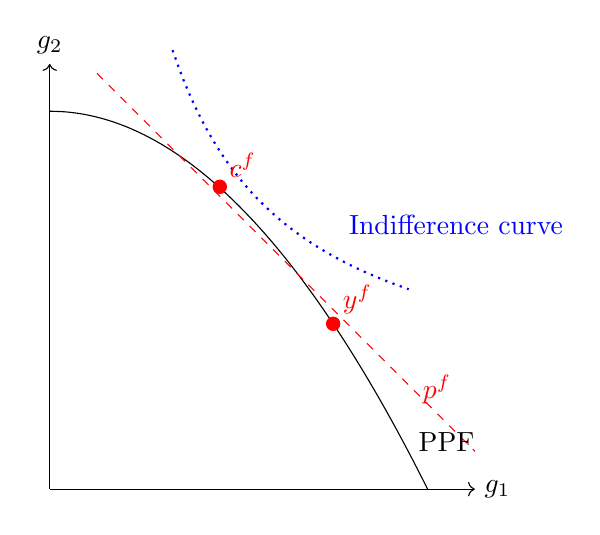
\begin{tikzpicture}[scale=1.2]
            % Define the PPF as a quadratic curve (same as in autarky)
            \draw[thin, domain=0:4, smooth, variable=\x] plot ({\x}, {4-0.25*\x*\x});
            
            % Higher indifference curve for free trade
            \draw[thick, blue, dotted, domain=1.3:3.8, smooth, variable=\x] plot ({\x}, {5/\x + 0.8});
            
            % World price line (different slope than autarky)
            \draw[dashed, red] (0.5,4.4) -- (4.5,0.4) node[pos=0.9, above] {$p^f$};
            
            % Production point (tangent to PPF with world prices)
            \filldraw[red] (3,1.75) circle (2pt) node[anchor=south west] {$y^f$};
            
            % Consumption point (tangent to indifference curve with world prices)
            \filldraw[red] (1.8,3.2) circle (2pt) node[anchor=south west] {$c^f$};
            
            % Axes
            \draw[->] (0,0) -- (4.5,0) node[right] {$g_1$};
            \draw[->] (0,0) -- (0,4.5) node[above] {$g_2$};
            
            % Labels
            \node at (4.2,0.5) {PPF};
            \node[blue] at (4.3,2.8) {Indifference curve};
        \end{tikzpicture}
        \caption{Free Trade Equilibrium}
    \end{subfigure}
    \caption{Equilibria for a Small Country}
    \label{fig:trade_equilibria}
\end{figure}

\subsubsection{Formula of Gains from Trade}
Arkolakis, Costinot, Rodriguez-Clare (AER, 2012)

\begin{assumption}
    \

    \begin{itemize}
        \item CES utility function(Dixit-Stiglitz)
        \[U = \left[\int q(\omega)^{\frac{\sigma -1}{\sigma}}\right]^{\frac{\sigma}{\sigma -1}}\] 
        \item One factor production(labor) and constant RS
        \item `Iceberg' trade costs
        \item Import demand system is CES: artial equilibrium (given wages)
        elasticity of aggregate bilateral trade flow relative to domestic
        demand is $\epsilon $ w.r.t. trade costs $\tau_{ij}$ fo any $i,j$.
    \end{itemize}
\end{assumption}

Define a “foreign shock” as any change in (foreign) endowments and
trade costs that do not affect a country's endowment or its ability to
serve its own market. Define $\hat{W} = \frac{W^{\prime}}{W}$ and $\hat{\lambda}_{jj} = \frac{\lambda_{jj}^{\prime} }{\lambda_{jj}}$

\begin{proposition}
    The change in country $j$'s real income associated with any foreign shock can be computed as $\hat{W}_{j} = \hat{\lambda}_{jj} ^{\frac{1}{\epsilon}}$,
    where $\lambda_{ij} $ is the share of country $j$'s spending on country $i$'s goods.
\end{proposition}

\begin{corollary}
    Gains from TRade relative to autarky can be computed as $\hat{W}_{j} = \lambda_{jj}^{-\frac{1}{\epsilon}} $.
\end{corollary}

\subsubsection{One household per country}
Consider first the case where there is just one household per country, $H=1$.
Without risk of confusion, we drop $h$ and $n$ from all variables.

We denote by:
\begin{itemize}
    \item $(y^a, c^a, p^a)$ the vector of output, consumption and good prices under autarky;
    \item $(y^f, c^f, p^f)$ the vector of output, consumption and good prices under free trade.
    \item $u^a$ and $u^f$ the utility levels under autarky and free trade.
\end{itemize}

\begin{proposition}\label{prop:1}
    \textit{In a neoclassical trade model with one household per country,
    free trade makes all households (weakly) better off.}
\end{proposition}

\begin{proof}
    \

    Under free trade, households can consume at prices $p^f$.
    By definition of the expenditure function, we have:
    \begin{align*}
        e(p^f, u^a) &\leq p^f c^a \\
        &= p^f y^a \\
        & \leq r(p^f, v^f) \\
        &= e(p^f, u^f)
    \end{align*}
    Since $e(p, \cdot)$ is increasing, we get $ u^f \geq u^a$.
\end{proof}

\begin{note}
    \

    \begin{itemize}
        \item Two inequalities in the previous proof correspond to consumption and
        production gains from trade.
        \item Previous inequalities are weak. Equality if kinks in IC or PPF.
        \item Previous proposition only establishes that households always prefer
        ``free trade'' to ``autarky.'' It \textbf{does not} say anything about the
        comparisons of trade equilibria.
    \end{itemize}
\end{note}

\subsubsection{Multiple households per country: domestic lump-sum transfers}
With multiple households per country, moving away from autarky is likely to create winners and losers.
In order to establish the Pareto-superiority of trade, we will need to allow for \textbf{policy instruments}.
We start with \textit{domestic lump-sum transfers} and then \textit{commodity taxes}.

We now reintroduce the index $h$ and denote by:
\begin{itemize}
    \item $c^{ah}$ and $c^{fh}$ the consumption vectors of household $h$ under autarky and free trade;
    \item $v^{ah}$ and $v^{fh}$ the endowment vectors of country $h$ under autarky and free trade;
    \item $u^{ah}$ and $u^{fh}$ the utility levels of household $h$ under autarky and free trade;
    \item $\tau^{h}$ the lump-sum transfer from the government to household $h$ under free trade.
    \footnote{$\tau ^h \leq 0 \Leftrightarrow$ lump-sum tax and $\tau ^h \geq 0 \Leftrightarrow$ lump-sum subsidy.}
\end{itemize}

\begin{proposition}\label{prop:2}
    \

    \textit{In a neoclassical trade model with multiple households per country,
    there exist domestic lump-sum transfers such that free trade is (weakly) Pareto superiority
    than autarky in all countries.}
\end{proposition}

\begin{proof}
    \

    For any $h$, set the lump-sum transfer $\tau^h$ such that:
    \[\tau ^h = (p^f - p^a)c^{ah} - (w^f - w^a)v^{fh}.\]
    Budget constraint unde rautarky implies that: $p^a c^{ah} \leq w^a v^{fh}. $
    Therefore, we have:
    \[p^f c^{ah} \leq w^f v^{fh} + \tau ^h.\]
    Thus $c^{ah} $ is still int he budget set of household $h$ under free trade.
    
    By definition, the government revenue is given by:
    \begin{align*}
        - \sum \tau ^h &= (p^a - p^f) \sum c^{ah} - (w^a - w^f) \sum v^{fh} \\
        &= (p^a - p^f) y^a - (w^a - w^f) v^f \\
        &= -p^f y^a + w^f v^f \\
        & \geq -r(p^f, v^f) + w^f v^f \\
        &= -(p^f y^f - w^f v^f) = 0.
    \end{align*}
\end{proof}

So, each household can buy its autarky consumption bundle at free trade prices and still have some money left.
But, the government must know individual preferences to implement the transfers.

If it does not, households can manipulate mechanism by altering their announcements or
autarky behavior. In other words, lump-sum transfers typically are
not \textcolor{red}{incentive compatible}.

\subsubsection{Multiple households per country: commodity taxes}
We now restrict the set of instruments to commodity taxes/subsidies.

Suppose that the government can affect the porices faced by households under free trade
by setting $\tau ^{good}$ and $\tau ^{factor}$:
\begin{align*}
    p^h &= p^f + \tau ^{good} \\
    w^h &= w^f + \tau ^{factor}.
\end{align*}

\begin{proposition}\label{prop:3}
    \

    \textit{In a neoclassical trade model with multiple households
    per country, there exist commodity taxes/subsidies such that free
    trade is (weakly) Pareto superior to autarky in all countries.}
\end{proposition}

\begin{proof}
    \

    Consider two following taxes:
    \begin{itemize}
        \item $\tau ^{good} = p^a - p^f$
        \item $\tau ^{factor} = w^a - w^f$
    \end{itemize}
    By construction, household is indifferent between autarky and free trade.
    Now consider the government revenue:
    \begin{align*}
        - \sum \tau ^h &= \sum \tau ^{good} c^{ah} - \sum \tau ^{factor} v^{fh} \\ 
        &= (p^a - p^f) \sum c^{ah} - (w^a - w^f) \sum v^{fh} \\
        &= (p^a - p^f) y^a - (w^a - w^f) v^f \\
        &= -p^f y^a + w^f v^f \\
        & \geq -r(p^f, v^f) + w^f v^f \\
        &= -(p^f y^f - w^f v^f) = 0.
    \end{align*}
\end{proof}

Tax revenue is non-negative. If all households are on the same side of the market
for at least for at least one good ot factor, government can cut a tax or raise a subsidy
to generate Pareto improvement.

This scheme sacrifices the consumer gains from trade,
but preserves the gains from reorganizing production.

\begin{note}
    \

    The previous proof only relies on existence of \textit{production gains} from trade.
    \begin{itemize}
        \item It's closely related to Diamod and Mirrlees (1971) result on the production efficiency
        \item When only commodity taxes are available, DM sho that production should remain efficient at a social optimum
        \item Thus, trade, acting as an expansion of PPF, should remain free(ignore issues of market power)
    \end{itemize}
    But, if there's a kink in the PPF, there are no production gains. \footnote{Similar problem with ``moving costs'', see Feenstra p. 185}

    Factor taxation still informationally intensive: need to know
endowments in efficiency units, may lead to different business taxes
\end{note}

\subsection{Law of Comparative Advantage}
The previous results have focused on normative predictions.
Let's take a look at how the same revealed preference argument can be used to make positive predictions about patterns of trade.

\begin{theorem}[Law of Comparative Advantage]\label{thm:LCA}
    \

    Countries tend to export goods in which they have a CA, i.e. lower
relative autarky prices compared to other countries    
\end{theorem}

\chapter{Ricardian Model}
\section{Introduction}

\subsection{Reasons of trade}
\begin{itemize}
    \item \textbf{Countries' differences: comparative advantage}
    \begin{itemize}
        \item Productivity: Ricardo
        \item Endowments: Heckscher-Ohlin
    \end{itemize}
    \item \textbf{Countries' similarities: economies of scale}
\end{itemize}

\subsection{Comparative advantage}
\begin{note}
    \

    Stanislaw Ulam's challenge to Paul Samuelson:  ``name me one
proposition in all of the social sciences which is both true and
non-trivial''. 

Samuelson's answer: Comparative advantage. ``That it is logically true need not be
argued before a mathematician; that is is not trivial is attested by
the thousands of important and intelligent men who have never
been able to grasp the doctrine for themselves or to believe it after
it was explained to them.''.\footnote{P.A. Samuelson (1969), ``The Way of an Economist,'' 
in P.A. Samuelson, ed., International Economic Relations: Proceedings of the Third Congress of the
International Economic Association, Macmillan: London, pp. 1-11.}
\end{note}

In the simplest and earliest complete model of production and trade,
the reason for trade is \textbf{comparative advantage}.
And the source of comparative advantage is \textbf{differences in production technologies}.

These are the differnces in production functions, not the differences
in labor productivities due to different endowments of capital which is the type of 
Heckscher-Ohlin model.

\subsection{Basic assumptions}
\begin{itemize}
    \item Labor is the only factor of production
    \item Constant returns to scale
    \item Perfect competition
    \item Full employment
    \item Endowments given, confined to country but intersectorally mobile
    within each country
    \item Two countries with different technologies (production functions)
    \item Number of goods: $n \geq 2$
\end{itemize}

\subsection{Technology}

\begin{question}
    How is efficiency measured?
\end{question}
With only one factor, we measure by the usage of the factor: \textbf{labbor requirement per unit output}.

We define the quantity of labour (e.g. number of hours) necessary
to produce one unit of good $i$ as $a_i$. If $a_i=2$, it means that 2 hours of labor
are needed to produce one unit of good $i$.

So, the labor productivity is the inverse of the labor requirement $a_i$, the higher the labor requirement, the lower the productivity.

\subsection{Production Possibility Frontier: Refresher}

PPF is the maximum possible production level for a given technology and factor endowment.
\begin{itemize}
    \item Constraint: points outside the PPF are not feasible;
    \item Efficiency: points inside the PPF are inefficient, those on the PPF are efficient;
    \item Opportunity cost: the slope of the PPF is the opportunity cost of producing one more unit of good $i$ in terms of good $j$.
    \item Concavity: the PPF is usually concave to the origin due to the law of diminishing returns.
\end{itemize}
Technology progress shifts the PPF outwards.

\section{The two-sector Model}

\subsection{A Simple Numerical Example}

Let's begin with a simple example: US and India producing corn and auto.
\begin{table}[htbp!]
    \centering
    \begin{tabular}{c|cc}
        \hline
        & US & India \\
        \hline
        Labor force & $L=200$ & $L^*=800$ \\
        Labor per unit corn & $a_c=8$ & $a_C^*=50$ \\
        Labor per unit auto & $a_A=10$ & $a_A^*=40$ \\
        \hline
    \end{tabular}
\end{table}

Specific assumption of this example : US is more
efficient/productive at producing both goods, meaning
US has an absolute advantage in both goods.

\subsubsection{Production Possibility Frontier}

\begin{minipage}{0.45\textwidth}
    \textbf{US}
    
    The full-employment condition is:
    \[
    L = a_{c}Q_{c} + a_{A}Q_{A}
    \]
    The PPF is a straight line connecting these two points:
    \[
    Q_A = \frac{L}{a_A} - \frac{a_C}{a_A}Q_C
    \]
    \centering
    \begin{tikzpicture}[scale=0.14]
        \draw[->] (0,0) -- (30,0) node[right] {$Q_C$};
        \draw[->] (0,0) -- (0,25) node[above] {$Q_A$};
            
            % PPF line
        \draw[thick, blue] (0,20) -- (25,0) node[midway, above, sloped]{};
            
        \node[below] at (25,0) {$25$};
        \node[left] at (0,20) {$20$};
            
    \end{tikzpicture}
    \captionof{figure}{US PPF}
\end{minipage}
\hfill
\begin{minipage}{0.45\textwidth}
    \textbf{India}
    
    The full-employment condition is:
    \[
    L^* = a_{C}^*Q_{C} + a_{A}^*Q_{A}
    \]

    The PPF is a straight line connecting these two points:
    \[
    Q_A^* = \frac{L^*}{a_A^*} - \frac{a_C^*}{a_A^*}Q_C
    \]
    \centering
    \begin{tikzpicture}[scale=0.14]
        \draw[->] (0,0) -- (30,0) node[right] {$Q_C^*$};
        \draw[->] (0,0) -- (0,25) node[above] {$Q_A^*$};
            
            % PPF line
        \draw[thick, red] (0,20) -- (16,0) node[midway, above, sloped]{};
        
        \node[below] at (16,0) {$16$};
        \node[left] at (0,20) {$20$};
    \end{tikzpicture}
    \captionof{figure}{India PPF}
\end{minipage}

\subsubsection{Relative price and Technology}

\begin{notation}
    \

    Relative price of corn: $P = \frac{P_C}{P_A}$;

    Relative quantity of corn: $Q = \frac{Q_C}{Q_A}$;

    $L$ and $L^*$ are the endowments of labor(in efficient units) in the two countries;

    $w$ and $w^*$ are the wage(in efficiency units) in the two countries.
\end{notation}

Workers are paid the value of their marginal products: $w_C = \frac{P_C}{a_C}$ and $w_A = \frac{P_A}{a_A}$.

Perfectly mobile labor: If both goods are produced, the wage in both sectors must be the same.
\[w_C = w_A \Leftrightarrow P = \frac{a_C}{a_A}.\]

\subsubsection{Production and Supply in the US}

If $P = \frac{a_C}{a_A} = 0.8$, the international price(relative price) is equal to the domestic opportunity cost of producing corn in terms of auto.
Trade cannot bring extra gains. Hence the production set doesn't affect the consumption set, and the production set can be anywhere on the PPF. $1 \leq \frac{Q_c}{Q_A} < \infty$. 

If $P < \frac{a_C}{a_A} = 0.8$, international price of C is lower than the domestic opportunity cost of producing C in terms of A. 
US will produce only A and import C. 
$Q_C = 0$, $Q_A = 20$, and $\frac{Q_C}{Q_A} = 0$.

If $P > \frac{a_C}{a_A} = 0.8$, international price of C is higher than the domestic opportunity cost of producing C in terms of A. 
US will produce only C and export A.
$Q_A = 0$, $Q_C = 25$, and $\frac{Q_C}{Q_A} = \infty$.

\begin{center}
\begin{tikzpicture}[scale=1.2]
    % Axes
    \draw[->] (0,0) -- (6,0) node[right] {$\frac{Q_C}{Q_A}$};
    \draw[->] (0,0) -- (0,4) node[above] {$P = \frac{P_C}{P_A}$};
    
    % Critical price line
    \draw[dashed] (0,1.6) -- (5.5,1.6) node[left] at (0,1.6) {$0.8 = \frac{a_C}{a_A}$};
    
    % Supply curve
    \draw[thick, blue] (0,0) -- (0,1.6) -- (5,1.6) -- (5,4);
    
    % Points for clarification
    \fill[blue] (0,1.6) circle (2pt);
    \fill[blue] (5,1.6) circle (2pt);
    
    % Labels
    \node[blue, left] at (0,0.8) {Only Autos ($Q_C=0, Q_A=20$)};
    \node[blue, below] at (2.5,1.6) {Both goods produced};
    \node[blue, right] at (5,2.5) {Only Corn ($Q_C=25, Q_A=0$)};
    
    % X-axis markers
    \node[below] at (0,0) {$0$};
    \node[below] at (5,0) {$\infty$};
\end{tikzpicture}
\captionof{figure}{US Relative supply}
\end{center}

\subsubsection{Autarky equilibria in the two countries}

\begin{minipage}{0.48\textwidth}
    \centering
    \begin{tikzpicture}[scale=1.2]
        % Axes
        \draw[->] (0,0) -- (4,0) node[right] {$\frac{Q_C}{Q_A}$};
        \draw[->] (0,0) -- (0,3) node[above] {$P = \frac{P_C}{P_A}$};
        
        % Critical price line
        \draw[dashed] (0,0.8) -- (3.7,0.8) node[left] at (0,0.8) {$0.8 = \frac{a_C}{a_A}$};
        
        % Supply curve
        \draw[thick, blue] (0,0) -- (0,0.8) -- (3.2,0.8) -- (3.2,2.8);
        
        % Points for clarification
        \fill[blue] (0,0.8) circle (2pt);
        \fill[blue] (3.2,0.8) circle (2pt);
        
        % Labels
        \node[blue, left, scale=0.7] at (0,0.4) {Only Autos};
        \node[blue, above, scale=0.7] at (1.6,0.8) {Both goods};
        \node[blue, right, scale=0.7] at (3.2,2) {Only Corn};
        
        % X-axis markers
        \node[below] at (0,0) {$0$};
        \node[below] at (5,0) {$\infty$};
    \end{tikzpicture}
    \captionof{figure}{US Relative Supply}
\end{minipage}
\hfill
\begin{minipage}{0.48\textwidth}
    \centering
    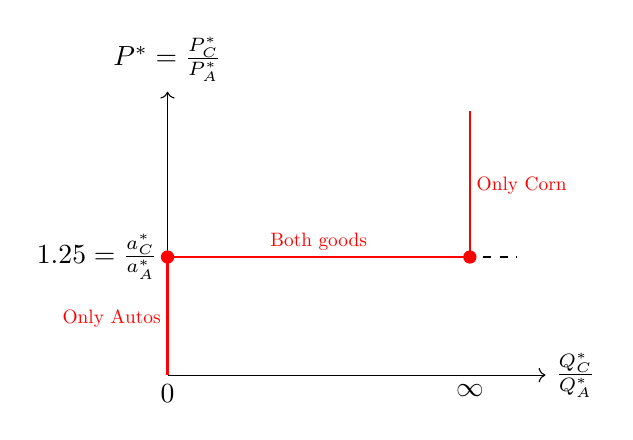
\begin{tikzpicture}[scale=1.2]
        % Axes
        \draw[->] (0,0) -- (4,0) node[right] {$\frac{Q_C^*}{Q_A^*}$};
        \draw[->] (0,0) -- (0,3) node[above] {$P^* = \frac{P_C^*}{P_A^*}$};
        
        % Critical price line
        \draw[dashed] (0,1.25) -- (3.7,1.25) node[left] at (0,1.25) {$1.25 = \frac{a_C^*}{a_A^*}$};
        
        % Supply curve
        \draw[thick, red] (0,0) -- (0,1.25) -- (3.2,1.25) -- (3.2,2.8);
        
        % Points for clarification
        \fill[red] (0,1.25) circle (2pt);
        \fill[red] (3.2,1.25) circle (2pt);
        
        % Labels
        \node[red, left, scale=0.7] at (0,0.6) {Only Autos};
        \node[red, above, scale=0.7] at (1.6,1.25) {Both goods};
        \node[red, right, scale=0.7] at (3.2,2) {Only Corn};
        
        % X-axis markers
        \node[below] at (0,0) {$0$};
        \node[below] at (3.2,0) {$\infty$};
    \end{tikzpicture}
    \captionof{figure}{India Relative Supply}
\end{minipage}

\subsubsection{Trade: Relative supply}

When we combine the two countries to form the world market, we get the following relative supply curve:

- When $P<0.8$, both countries produce only autos, world ratio $R = 0$.

- When $P=0.8$, US can vary production between 20 autos, 
no corn (world $R = 0$), and 0 autos, 25 corn (world
$R = 1.25$) while India produces only autos, so world $R \in [0, 1.25]$.

- When $0.8<P<1.25$, US produces only corn, India produces only autos, so $R = \frac{25}{20} = 1.25$.

- When $P=1.25$, India can vary production while US produces only corn, so world $R \in \left. \left[ 1.25, \infty \right. \right)$.

- When $P>1.25$, both countries produce only corn, so world $R = \infty$.

\begin{center}
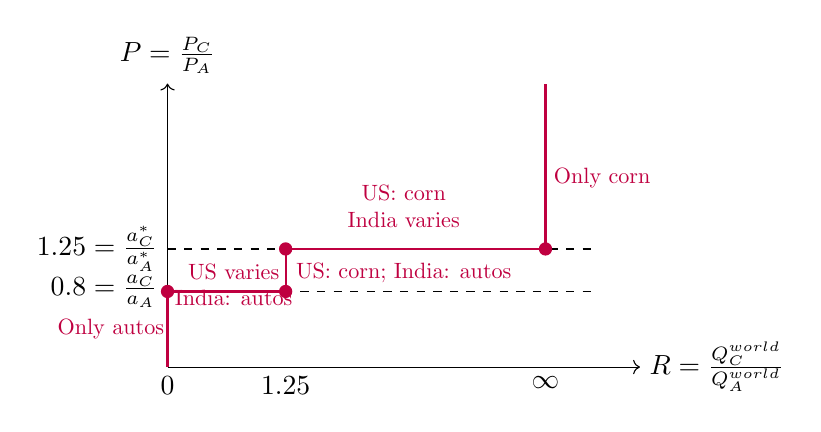
\begin{tikzpicture}[scale=1.2]
    % Axes
    \draw[->] (0,0) -- (5,0) node[right] {$R = \frac{Q_C^{world}}{Q_A^{world}}$};
    \draw[->] (0,0) -- (0,3) node[above] {$P = \frac{P_C}{P_A}$};
    
    % Critical price lines
    \draw[dashed] (0,0.8) -- (4.5,0.8) node[left] at (0,0.8) {$0.8 = \frac{a_C}{a_A}$};
    \draw[dashed] (0,1.25) -- (4.5,1.25) node[left] at (0,1.25) {$1.25 = \frac{a_C^*}{a_A^*}$};
    
    % World Relative Supply curve
    \draw[thick, purple] (0,0) -- (0,0.8) -- (1.25,0.8) -- (1.25,1.25) -- (4,1.25) -- (4,3);
    
    % Points for clarification
    \fill[purple] (0,0.8) circle (2pt);
    \fill[purple] (1.25,0.8) circle (2pt);
    \fill[purple] (1.25,1.25) circle (2pt);
    \fill[purple] (4,1.25) circle (2pt);
    
    % Region labels
    \node[purple, scale=0.8, align=left] at (-0.6,0.4) {Only autos};
    \node[purple, scale=0.8, align=center] at (0.7,0.87) {US varies\\India: autos};
    \node[purple, scale=0.8, align=center] at (2.5,1) {US: corn; India: autos};
    \node[purple, scale=0.8, align=center] at (2.5,1.7) {US: corn\\India varies};
    \node[purple, scale=0.8, align=right] at (4.6,2) {Only corn};
    
    % X-axis markers
    \node[below] at (0,0) {$0$};
    \node[below] at (1.25,0) {$1.25$};
    \node[below] at (4,0) {$\infty$};
\end{tikzpicture}
\captionof{figure}{World Relative Supply Curve}
\end{center}

\subsubsection{Trading Equilibrium}

Depending on position of relative demand, the trading equilibrium can be one of three types:
\begin{itemize}
    \item[A.] $P=0.8$, US produces both goods, India produces only autos;
    \item[B.] $0.8<P<1.25$, US produces only corn, India produces only autos;
    \item[C.] $P=1.25$, US produces only corn, India produces both goods.
\end{itemize}

\begin{center}
    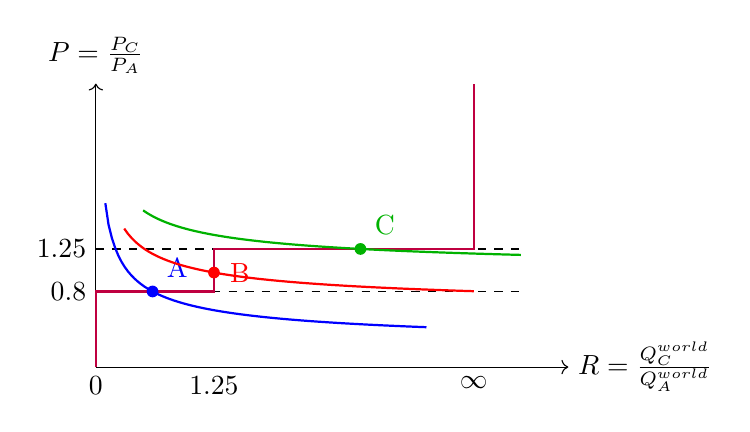
\begin{tikzpicture}[scale=1.2]
        % Axes
        \draw[->] (0,0) -- (5,0) node[right] {$R = \frac{Q_C^{world}}{Q_A^{world}}$};
        \draw[->] (0,0) -- (0,3) node[above] {$P = \frac{P_C}{P_A}$};
        
        % Critical price lines
        \draw[dashed] (0,0.8) -- (4.5,0.8) node[left] at (0,0.8) {$0.8$};
        \draw[dashed] (0,1.25) -- (4.5,1.25) node[left] at (0,1.25) {$1.25$};
        
        % World Relative Supply curve
        \draw[thick, purple] (0,0) -- (0,0.8) -- (1.25,0.8) -- (1.25,1.25) -- (4,1.25) -- (4,3);
        
        % New equilibrium points (adjusted)
        \node[circle, fill, blue, inner sep=1.5pt, label={[blue]above right:A}] at (0.6,0.8) {};
        \node[circle, fill, red, inner sep=1.5pt, label={[red]right:B}] at (1.25,1.0) {};
        \node[circle, fill, green!70!black, inner sep=1.5pt, label={[green!70!black]above right:C}] at (2.8,1.25) {};
        
        % Indifference curves (parallel)
        % Curve A passing through (0.6,0.8)
        \draw[blue, thick] plot[domain=0.1:3.5, samples=100] (\x, {0.5 * pow(\x, -0.5) + 0.1545});
        
        % Curve B passing through (1.25,1.0)
        \draw[red, thick] plot[domain=0.3:4, samples=100] (\x, {0.5 * pow(\x, -0.5) + 0.5528});
        
        % Curve C passing through (2.8,1.25)
        \draw[green!70!black, thick] plot[domain=0.5:4.5, samples=100] (\x, {0.5 * pow(\x, -0.5) + 0.9512});
        
        % X-axis markers
        \node[below] at (0,0) {$0$};
        \node[below] at (1.25,0) {$1.25$};
        \node[below] at (4,0) {$\infty$};
    \end{tikzpicture}
    \captionof{figure}{Trading Equilibrium}
\end{center}

\subsubsection{Efficient production and world PPF}

Suppose initially all labor produc autos in both: 40 in all.
If any corn is produced, it's better to do so by switching sone labor in the US:
because wach auto not produced releases 10 labor which can then produce 1.25 corn,
while in India, each less auto yields only 0.8 more corn.

Only when all US labor has been diverted to producing corn
should any Indian labor be switched.

Conversely, starting with all corn: 41 units, to produce any autos,
Indian labor should be switched.

This despite the US producing autos more efficiently than India: only
10 units of labor against 40. The reason: the US produces corn even
more efficiently: only 8 units of labor against 50. What matters is the
ratio (opportunity cost): $\frac{10}{8} > \frac{40}{50}$, or $\frac{10}{40} > \frac{8}{50}$.

\begin{center}
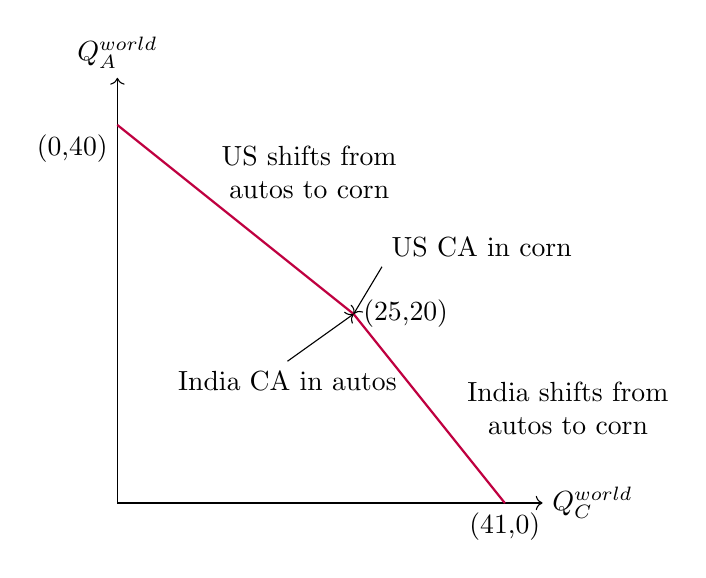
\begin{tikzpicture}[scale=0.12]
    % Axes
    \draw[->] (0,0) -- (45,0) node[right] {$Q_C^{world}$};
    \draw[->] (0,0) -- (0,45) node[above] {$Q_A^{world}$};
    
    % World PPF
    \draw[thick, purple] (0,40) -- (25,20) -- (41,0);
    
    % Points for clarification
    \fill[purple] (0,40) circle (2pt);
    \fill[purple] (25,20) circle (2pt);
    \fill[purple] (41,0) circle (2pt);
    
    % Labels for key points
    \node[below left] at (0,40) {(0,40)};
    \node[right] at (25,20) {(25,20)};
    \node[below] at (41,0) {(41,0)};
    
    % Production allocation labels
    \node[right, align=center] at (10,35) {US shifts from\\autos to corn};
    \node[right, align=center] at (36,10) {India shifts from\\autos to corn};
    
    % Efficiency regions
    \node[below left, purple] at (0,40) {};
    \node[right, purple] at (25,20) {};
    \node[above right, purple] at (41,0) {};
    
    % Country labels for the kink point
    \draw[->] (28,25) -- (25,20);
    \node[above right] at (28,25) {US CA in corn};
    \draw[->] (18,15) -- (25,20);
    \node[below] at (18,15) {India CA in autos};
\end{tikzpicture}
\captionof{figure}{World Production Possibility Frontier}
\end{center}

\subsubsection{TRading equilibrium and world PPF}

If preferences are identical and homthetic everywhere, we can draw the world indifference curves.
Depending on their shape, there are three types of outcomes:
\begin{itemize}
    \item[A.] US produces both goods, India produces only autos;
    \item[B.] US produces only corn, India produces only autos;
    \item[C.] US produces only corn, India produces both goods.
\end{itemize}

Relative price of corn $=$ slope of PPF: 0.8 in A, 1.25 in C, between 0.8 and 1.25 in B.

\begin{center}
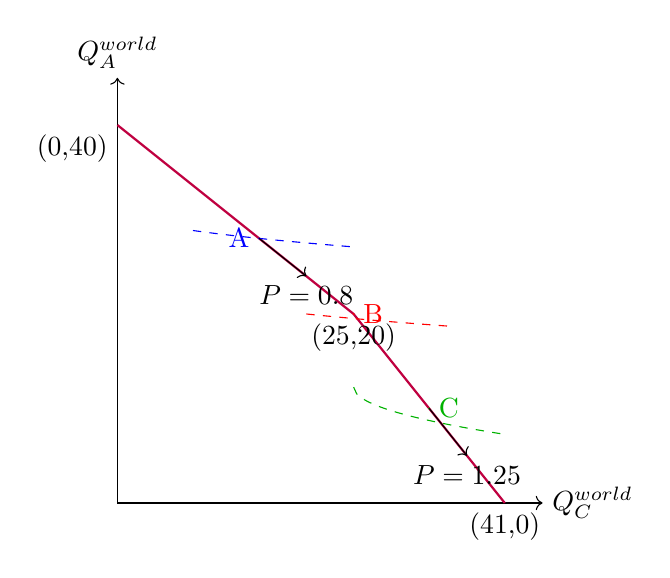
\begin{tikzpicture}[scale=0.12]
    % Axes
    \draw[->] (0,0) -- (45,0) node[right] {$Q_C^{world}$};
    \draw[->] (0,0) -- (0,45) node[above] {$Q_A^{world}$};
    
    % World PPF
    \draw[thick, purple] (0,40) -- (25,20) -- (41,0);
    
    % Equilibrium points
    \fill[blue] (15,28) circle (3pt) node[left] {A};
    \fill[red] (25,20) circle (3pt) node[right] {B};
    \fill[green!70!black] (33,10) circle (3pt) node[right] {C};
    
    % Indifference curves
    \draw[blue, dashed] plot[domain=8:25, samples=50] (\x, {31.1 - 0.8*sqrt(\x)});
    \draw[red, dashed] plot[domain=20:35, samples=50] (\x, {23.1 - 0.8*sqrt(\x-5)});
    \draw[green!70!black, dashed] plot[domain=25:41, samples=50] (\x, {12.263 - 1.25*sqrt(\x-25)});
    
    % Labels for key points
    \node[below left] at (0,40) {(0,40)};
    \node[below] at (25,20) {(25,20)};
    \node[below] at (41,0) {(41,0)};
    
    % Production allocations
    \node[blue, above, align=center] at (15,28) {};
    \node[red, below left, align=center] at (25,20) {};
    \node[green!70!black, above, align=center] at (33,10) {};
    
    % Price lines
    \draw[->, thin] (15,28) -- (20,24);
    \node[below] at (20,24) {$P=0.8$};
    
    % \draw[->, thin] (25,20) -- (30,17);
    % \node[below] at (30,17) {$0.8<P<1.25$};
    
    \draw[->, thin] (33,10) -- (37,5);
    \node[below] at (37,5) {$P=1.25$};
\end{tikzpicture}
\captionof{figure}{Trading Equilibrium on the World PPF}
\end{center}

% \chapter{Hypothesis Testing}
% \section{Some Basic Concepts}

\begin{definition}
    \textbf{\textcolor{blue}{Null Hypothesis}}
    
    The null hypothesis $\mathcal{H}_0$ is the set $\theta = \theta_0$ or $\beta \in \mathcal{B}_0$.
    
    Or, we denote it as:
    \[ \mathcal{H}_0 : \theta \in \Theta_0 \]
    For econometrics, we usually set $\mathcal{H}_0 : \beta = 0$.
\end{definition}

\begin{definition}
    \textbf{\textcolor{blue}{Alternative Hypothesis}}
    
    The alternative hypothesis $\mathcal{H}_1$ is the set $\{ \theta \in \Theta : \theta \neq \theta_0 \}$ or $\{ \beta \in \mathcal{B} : \beta \notin \mathcal{B}_0 \}$.
    
    Or, we denote it as:
    \[ \mathcal{H}_1 : \theta \in \Theta_1 \]
    For econometrics, we usually set $\mathcal{H}_1 : \beta \neq 0$. Often $\Theta_1$ is the complement of $\Theta_0$.
\end{definition}

\begin{note}
    Point estimator of $\mathbf{1} \{ \theta \in \Theta_0 \}$ (if $\theta \in \Theta_0$, the function equals 1).
\end{note}

\begin{center}
    \begin{tabular}{|c|c|c|}
        \hline
        & $\mathcal{H}_0$ is true & $\mathcal{H}_0$ is false\\
        \hline
        Accept $\mathcal{H}_0$ & $\checkmark$: $1 - \alpha$ & $\times$: $1 - \beta$\\
        \hline
        Reject $\mathcal{H}_0$ & $\times$: $\alpha$ & $\checkmark$: $\beta$\\
        \hline
    \end{tabular}
\end{center}

$\alpha$ is the Type I error, $1 - \beta$ is the Type II error.

\begin{definition}
    A hypothesis test $\varphi \in \{0, 1\}$ is a rule that specifies when we reject and when we accept (do not reject) $\mathcal{H}_0$, with $\varphi = 0$ indicating rejection.
\end{definition}

\begin{definition}
    \textbf{Power Function}
    \[ \beta (\theta) = \mathbb{P} [\text{rejecting} | \theta \text{ is} \text{ true}] = \mathbb{P} [\varphi = 0 | \theta] \]
\end{definition}

\begin{definition}
    \textbf{Size of a test}
    
    The size of a test is $\alpha$ if $\underset{\theta \in \Theta_0}{\sup} \beta (\theta_0) = \alpha$, $\alpha \in (0, 1)$.
\end{definition}

\textit{Generic form:}
\[ \varphi (x ; \alpha) = \mathbf{1} \{ T (x) < c_{\alpha} \} \]

\section{T-test}

\begin{definition}
    Suppose $\hat{\theta} | \theta \sim N (\theta, v^2)$, and we are testing a point hypothesis $\mathcal{H}_0 : \theta = \theta_0$. Under the alternative $\mathcal{H}_1 : \theta \neq \theta_0$, the two-sided t-test is
    \[ \varphi_t (x) = \mathbf{1} \left\{ \left| \frac{\hat{\theta} - \theta_0}{v} \right| < c \right\} \]
\end{definition}

\begin{note}
    The test-statistic $T (X) = \left| \frac{\hat{\theta} - \theta_0}{v} \right|$ is a function of data $X$ because our estimator $\theta$, $\hat{\theta}$, is a function of $X$.
\end{note}

\begin{eg}
    Let $X | \theta \sim N (\theta, v^2)$, under $\mathcal{H}_0 : \hat{\theta} \sim N (\theta_0, v^2)$ $\rightarrow$ $\frac{\hat{\theta} - \theta_0}{v} \sim N (0, 1)$
\end{eg}

\includegraphics[width=\textwidth]{t-test.pdf}

\begin{align*}
    \beta (\theta) & = \mathbb{P} [\text{rejecting} | \theta \text{ is} \text{ true}]\\
    & = \mathbb{P} [\varphi = 0 | \theta]\\
    & = \mathbb{P} [T (X) > c_{\alpha} | \theta]\\
    & = \mathbb{P} \left[ \left| \frac{\hat{\theta} - \theta_0}{v} \right| > c_{\alpha} | \theta \right]\\
    & = 1 - \mathbb{P} \left[ \left| \frac{\hat{\theta} - \theta_0}{v} \right| \leq c_{\alpha} | \theta \right]\\
    & = 1 - \mathbb{P} \left[ - c_{\alpha} \leq \frac{\hat{\theta} - \theta_0}{v} \sim N (0, 1) \leq c_{\alpha} | \theta \right]\\
    & = 1 - \left( \mathbb{P} \left[ \frac{\hat{\theta} - \theta_0}{v} \leq c_{\alpha} | \theta \right] - \mathbb{P} \left[ \frac{\hat{\theta} - \theta_0}{v} \leq - c_{\alpha} | \theta \right] \right)\\
    & = 1 - [\Phi (c_{\alpha}) - \Phi (- c_{\alpha})]\\
    & = 1 - [\Phi (c_{\alpha}) - (1 - \Phi (c_{\alpha}))]\\
    & = 2 - 2 \Phi (c_{\alpha})\\
    & = \alpha
\end{align*}

Under $\alpha = 0.05$, we get $c_{\alpha} = 1.64$, $\alpha = 0.1$, we get
$c_{\alpha} = 1.96$.

To compute the power of this test, we need to think about what happens if
$\mathcal{H}_0$ is false. Assuming that $\tilde{\theta}$ is the true value of
$\theta$.

\begin{align*}
  \beta (\tilde{\theta}) & = \mathbb{P} [\text{rejecting} |
  \tilde{\theta} \text{ is true}]\\
  & = \mathbb{P} [\varphi = 0 | \tilde{\theta}]\\
  & = \mathbb{P} [T (X) > c_{\alpha} | \tilde{\theta}]\\
  & = \mathbb{P} \left[ \left| \frac{\hat{\theta} - \theta_0}{v} \right| >
  c_{\alpha} | \tilde{\theta} \right]
\end{align*}

To find this, under $\tilde{\theta}$ is true, $\tilde{\theta} \sim N
(\tilde{\theta}, v^2)$, $\hat{\theta} - \tilde{\theta} \sim N (0, v^2)$,
$\hat{\theta} - \theta_0 \sim N (\tilde{\theta} - \theta_0, v^2)$,
$\frac{\hat{\theta} - \theta_0}{v} \sim N (\tilde{\theta} - \theta_0, 1)$,
$\frac{\hat{\theta} - \theta_0}{v} - (\tilde{\theta} - \theta_0) \sim N (0,
1)$

So,
\begin{align*}
  \beta (\tilde{\theta}) & = \mathbb{P} \left[ \left| \frac{\hat{\theta} -
  \theta_0}{v} \right| > c_{\alpha} | \tilde{\theta}
  \right]\\
  & = 1 - \mathbb{P} \left[ \left| \frac{\hat{\theta} - \theta_0}{v}
  \right| \leq c_{\alpha} | \theta \right]\\
  & = 1 - \mathbb{P} \left[ - c_{\alpha} \leq \frac{\hat{\theta} -
  \theta_0}{v} \leq c_{\alpha} | \theta \right]\\
  & = 1 - \mathbb{P} [- c_{\alpha} - (\tilde{\theta} - \theta_0) \leq z
  \sim N (0, 1) \leq c_{\alpha} - (\tilde{\theta} - \theta_0)]\\
  & = 1 - (\Phi [c_{\alpha} - (\tilde{\theta} - \theta_0)] - \Phi [-
  c_{\alpha} - (\tilde{\theta} - \theta_0)])
\end{align*}

The higher the probability of wrongly accepting (or failing to reject)
$\mathcal{H}_0$. It is common to be rather conservative (i.e. erring on the
side of not rejecting $\mathcal{H}_0$) and report test results for sizes of
10\%, 5\% and 1\%.

\section{Likelihood Ratio Test}

\begin{definition}
  \[ \varphi_{\text{LR}} (x) = \mathbf{1} \left\{ \frac{\underset{\theta \in
     \Theta_1}{\sup} p (x | \theta)}{\underset{\theta \in
     \Theta_0}{\sup} p (x | \theta)} < c_{\alpha} \right\},
     T_{\text{LR}} (X) = \frac{\underset{\theta \in \Theta_1}{\sup} p (x |
  \theta)}{\underset{\theta \in \Theta_0}{\sup} p (x | \theta)}.\]
\end{definition}

So, if there are points in $\Theta_0$ for which observed $x$ is more likely
than points in $\Theta_1$, the ratio is small --- the test is likely to accept
$\mathcal{H}_0$.

Under $\mathcal{H}_0 : \theta = \theta_0$ and the alternative $\mathcal{H}_1 :
\theta \neq \theta_0$,
\[ \varphi_{\text{LR}} (x) = \mathbf{1} \left\{ \frac{p (x |
   \hat{\theta}_{\text{ML}})}{p (x | \theta_0)} < c \right\} \]

\begin{eg}
  $\{ x_i \}_{i = 1}^n$, $x_i | \theta \sim N (\theta, 1)$,
  \[ p (x | \theta) = \prod_i p (x_i | \theta) = (2
     \pi)^{- \frac{1}{2}} \exp \left\{ - \frac{1}{2} (x - \theta)^2 \right\}
  \]
  if $n = 1$. As $x = \hat{\theta}$, $p (x | \hat{\theta}) = (2
  \pi)^{- \frac{1}{2}}$
  \[ T (x) = \frac{p (x | \hat{\theta}_{\text{ML}})}{p (x |
     \theta_0)} = \frac{(2 \pi)^{- \frac{1}{2}} \exp \left\{ -
     \frac{1}{2} (x - \hat{\theta})^2 \right\}}{(2 \pi)^{- \frac{1}{2}} \exp
     \left\{ - \frac{1}{2} (x - \theta_0)^2 \right\}} = \exp \left\{
     \frac{1}{2} (x - \theta_0)^2 \right\} \]
  as $x = \hat{\theta}$.
  \[ \varphi_{\text{LR}} = \mathbf{1} \left\{ \exp \left\{ \frac{1}{2} (x -
     \theta_0)^2 \right\} < c_{\alpha} \right\} \]
\end{eg}

\begin{align*}
  \alpha & = \mathbb{P} \{ \text{Reject} | \theta_0 \text{ is}
  \text{ actually true} \}\\
  & = \mathbb{P} \left\{ \exp \left\{ \frac{1}{2} (x - \theta_0)^2 \right\}
  \geq c_{\alpha} | \theta_0 \right\}\\
  & = \mathbb{P} \{ (x - \theta_0)^2 \geq 2 \log c_{\alpha} |
  \theta_0 \}\\
  & = 1 - \mathbb{P} \left\{ (x - \theta_0)^2 <
  2 \log c_{\alpha} | \theta_0 \right\}
\end{align*}

If $x \sim N (\theta_0, 1)$, $(x - \theta_0)^2 \sim \chi_{1}^2$

\includegraphics[width=\textwidth]{Chi-2.pdf}

\begin{note}
  \textbf{\textcolor{red}{Uniformly most powerful test}} Highest probability
  of rejection, of wrong acceptance.
\end{note}

\[ \varphi (x) = \mathbf{1} \{ T (x) < c_{\alpha} \} \]
\[ \alpha = \mathbb{P} \{ T (x) > c_{\alpha} | \theta_0 \} 
   (\text{reject rule}) \]

\subsection{Numerical Hypothesis Testing}

\begin{algorithm}[H]
  \caption{Numerical Hypothesis Testing}
  \SetAlgoLined
  \SetKwInOut{Input}{Input}
  \SetKwInOut{Output}{Output}
  
  \Input{Distribution $N(\theta_0, 1)$, sample size $M$, significance level $\alpha$}
  \Output{Decision to accept or reject $H_0$}
  
  \For{$m = 1$ \KwTo $M$}{
      Draw $x^m \sim N(\theta_0, 1)$\;
      Compute $T(x^m)$\;
  }
  
  Sort $\{T(x^m)\}_{m=1}^M$ in ascending order\;
  Set $c_\alpha$ to the $100(1 - \alpha)$ quantile of $\{T(x^m)\}_{m=1}^M$\;
  
  Compute $T(x)$ for your observed realization $x$\;
  \eIf{$T(x) \leq c_\alpha$}{
      Accept $H_0$\;
  }{
      Reject $H_0$\;
  }
\end{algorithm}

Small $p\text{-value}$ means $\mathcal{H}_0$ is likely to be rejected,
larger $p\text{-value}$ means it's likely to be true.

\section{Coverage Sets}

\subsection{Frequentist Confidence Sets}

A confidence set $C (X) \subseteq \Theta$ is a (random) set that should cover
the true $\theta$ with a prespecified probability:
\[ \underset{\theta \in \Theta}{\inf} \mathbb{P} [\theta \in C (X) |
   \theta] = 1 - \alpha \]
\[ C (x) = \{ \theta_0 \in \Theta : \varphi (x ; \theta_0) = 1 \} \]
contains all the values of $\theta_0$ that we would accept.

Consider $\mathcal{H}_0 : \theta = \theta_0$ vs. $\mathcal{H}_1 : \theta \neq
\theta_0$, $\varphi_{\alpha} (x) = \mathbf{1} \{ T (x) < c_{\alpha ; \theta_0}
\}$.

\begin{eg}
  T-test: $T (x) = \left| \frac{\hat{\theta} - \theta_0}{v} \right|$
  $\Rightarrow$ $\varphi \{ x ; \theta_0, \alpha \} = \mathbf{1} \{ T (x) < c
  \}$
  \begin{align*}
    C (x) & = \{ \theta_0 \in \Theta, \varphi \{ x ; \theta_0, \alpha \} = 1
    \}\\
    & = \left\{ \theta_0 \in \Theta, \left| \frac{\hat{\theta} -
    \theta_0}{v} \right| < c \right\}\\
    & = \left\{ \theta_0 \in \Theta, - c < \frac{\hat{\theta} -
    \theta_0}{v} < c \right\}\\
    & = \{ \theta_0 \in \Theta, - c v + \hat{\theta} < \theta_0 < c v +
    \hat{\theta} \}
  \end{align*}
\end{eg}

\begin{eg}
  LR-test: $\varphi (x ; \theta_0, \alpha) = \mathbf{1} \{ (x - \theta_0)^2 <
  \tilde{c_{\alpha}} \}$
  \begin{align*}
    C (x) & = \{ \theta_0 \in \Theta, \varphi \{ x ; \theta_0, \alpha \} = 1
    \}\\
    & = \{ \theta_0 \in \Theta, (x - \theta_0)^2 < \tilde{c_{\alpha}}
    \}\\
    & = \left\{ \theta_0 \in \Theta, - \sqrt{\tilde{c_{\alpha}}} < x -
    \theta_0 < \sqrt{\tilde{c_{\alpha}}} \right\}\\
    & = \left\{ \theta_0 \in \Theta, x - \sqrt{\tilde{c_{\alpha}}} <
    \theta_0 < x + \sqrt{\tilde{c_{\alpha}}} \right\}
  \end{align*}
\end{eg}

\subsection{Numerical Confidence Set Construction}

\begin{algorithm}[H]
  \caption{Numerical Confidence Set Construction}
  \SetAlgoLined
  
  \KwData{Choose a grid $\mathcal{T}$ of values for $\theta_0$}
  \For{each $\theta_0 \in \mathcal{T}$}{
    \For{$m = 1$ \KwTo $M$}{
        Draw $x^m \sim N(\theta_0, 1)$ \tcp*{Distribution of $X$ under $H_0 : \theta = \theta_0$}
        Compute $T(x^m, \theta_0)$\;
    }

    Get the critical value $c_\alpha(\theta_0)$ as the $(1-\alpha)$th quantile of $\{T(x^m, \theta_0)\}_{m=1}^M$\;
    Compute $T(x; \theta_0)$ for observed $x$\;
    
    \eIf{$T(x; \theta_0) \leq c_\alpha(\theta_0)$}{
        $\theta_0 \in C(x)$\;
    }{
        $\theta_0 \not\in C(x)$\;
    }
  }
\end{algorithm}
% \chapter{Problem Set 2}
% \begin{solution}
    \

   \textbf{Step 1:} Write the pdf of observations $x_i | \theta$
   
   Since $x_i = \theta + u_i$, and we assume $u_i \sim \mathcal{N}(0, \sigma^2)$, then $x_i \sim \mathcal{N}(\theta, \sigma^2)$, and we have:
   \[
   p(x_i | \theta) = \frac{1}{\sqrt{2\pi\sigma^2}} \exp{\left\{-\frac{1}{2} \frac{(x_i - \theta)^2}{\sigma^2}\right\}}.
   \]

   \textbf{Step 2:} Define Likelihood Function

   We have assumed that observations in the sample are independent. Thus, 
   \[
   L_n(\theta) = \prod\limits_{i=1}^{n}p(x_i | \theta) = \left(\frac{1}{\sqrt{2\pi\sigma^2}}\right)^n \exp{\left\{-\frac{1}{2\sigma^2} \sum_{i=1}^{n} (x_i - \theta)^2\right\}}
   \]
   Log-linearize the function, and we define the log-likelihood function:
   \[
   \ell_{n}(\theta) = n\log{\left(\frac{1}{\sqrt{2\pi\sigma^2}}\right)} - \frac{1}{2\sigma^2} \sum_{i=1}^{n}(x_i - \theta)^2
   \]

   \textbf{Step 3:} Define the Likelihood Estimation problem and find the $\hat{\theta}$

   For maximum likelihood estimation, we need to solve the following problem:
   \[
       \hat{\theta}_{ML} = \arg\max\limits_{\theta \in \Theta}{L_n(\theta)} = \arg\max\limits_{\theta \in \Theta}{\ell_n(\theta)}
   \]
   So, we need to maximize:
   \[
   \ell_{n}(\theta) = n\log{\left(\frac{1}{\sqrt{2\pi\sigma^2}}\right)} - \frac{1}{2\sigma^2} \sum_{i=1}^{n}(x_i - \theta)^2
   \]
   Take the derivative of $\ell_n(\theta)$ with respect to $\theta$, and set it to zero for maximization,
   \begin{align*}
       \frac{\partial \ell_n(\theta)}{\partial \theta} &= \frac{1}{\sigma^2} \sum_{i=1}^{n}(x_i - \theta) \\
       &= \frac{1}{\sigma^2}(\sum_{i=1}^{n}x_i - n\theta) \\
       &= 0
   \end{align*}
   Thus, we have
   \[
   \hat{\theta}_{ML} = \frac{1}{n}\sum_{i=1}^{n}x_i
   \]
   
\end{solution}

\begin{solution}
    \ 

    \textbf{Step 1:} Find the likelihood function
    
    For $\mathcal{H}_0: \theta = \theta_0$, the likelihood function is:
    \[
    L_n(\theta_0) = \left(\frac{1}{\sqrt{2\pi\sigma^2}}\right)^n \exp{\left\{-\frac{1}{2\sigma^2} \sum_{i=1}^{n} (x_i - \theta_0)^2\right\}}
    \]
    For $\mathcal{H}_1: \theta \neq \theta_0$, the maximum likelihood estimator is $\hat{\theta}_{ML} = \frac{1}{n}\sum\limits_{i=1}^{n}x_i = \hat{\theta}$. The likelihood function is:
    \[
    L_n(\theta_1) = \left(\frac{1}{\sqrt{2\pi\sigma^2}}\right)^n \exp{\left\{-\frac{1}{2\sigma^2} \sum_{i=1}^{n} (x_i - \hat{\theta})^2\right\}}
    \]

    \textbf{Step 2:} Define the likelihood ratio test and $c_\alpha$

    The likelihood ratio and the test is firstly defined as follows(we'll simplify to another version later):
    \[
    \varphi_{LR}(x) = \mathbf{1}\left\{LR_n < c\right\}
    \]
    \begin{align*}
         LR_n &= \frac{L_n(\theta_1)}{L_n(\theta_0)} \\
              &= \exp{\left\{ \frac{1}{2\sigma^2}\left[\sum_{i=1}^{n} (x_i - \theta_0)^2 - \sum_{i=1}^{n} (x_i - \hat{\theta})^2\right]\right\}}
    \end{align*}
    Denote 
    \[
    D = \sum\limits_{i=1}^{n} (x_i - \theta_0)^2 - \sum\limits_{i=1}^{n} (x_i - \hat{\theta})^2
    \]
    Using the identity:
    \[
    \sum\limits_{i=1}^{n} (x_i - \theta_0)^2 = \sum\limits_{i=1}^{n} (x_i - \hat{\theta} + \hat{\theta} - \theta_0)^2 = \sum\limits_{i=1}^{n} (x_i - \hat{\theta})^2 + n(\hat{\theta} - \theta_0)^2
    \]
    Thus, 
    \begin{align*}
        D &= \sum\limits_{i=1}^{n} (x_i - \theta_0)^2 - \sum\limits_{i=1}^{n} (x_i - \hat{\theta})^2 \\
          &= \sum\limits_{i=1}^{n} (x_i - \hat{\theta})^2 + n(\hat{\theta} - \theta_0)^2 - \sum\limits_{i=1}^{n} (x_i - \hat{\theta})^2 \\
          &= n(\hat{\theta} - \theta_0)^2
    \end{align*}
    So, the likelihood ratio $LR_n$ is:
    \[
    LR_n = \exp{\left\{\frac{n}{2\sigma^2} (\hat{\theta} - \theta_0)^2\right\}}
    \]
    Then, we simplify the expression and define the test statistic $T(x)$ as below:
    \[
    T(x) = 2\log{(LR_n)} = \frac{n}{\sigma^2}(\hat{\theta} - \theta_0)^2
    \]
    And our LR test would be:
    \[
    \varphi_{LR}(x) = \mathbf{1}\left\{ T(x) = \frac{n}{\sigma^2}(\hat{\theta} - \theta_0)^2 < c'\right\}
    \]
    where $c' = 2\log(c)$.
    To get a size $\alpha$ test, we find $c'$ so as to set the Type I error to $\alpha$, which is:
    \[
    \mathbb{P}\left[ T(x) \geq c' | \mathcal{H}_0\right] = \alpha
    \]
    we can denote that $c' = c_\alpha$.

    \textbf{Step 3:} Determine the distribution of $T(x)$ under $\mathcal{H}_0$ and find the value of $c_\alpha$

    Under $\mathcal{H}_0$, $\hat{\theta} \sim \mathcal{N}(\theta_0, \frac{\sigma^2}{n})$, because:
    \begin{align*}
        \mathbb{E}[\hat{\theta}] &= \mathbb{E}\left[\frac{1}{n}\sum\limits_{i=1}^{n}x_i\right] = \frac{1}{n}\sum\limits_{i=1}^{n}\mathbb{E}[x_i] = \frac{1}{n}\cdot n\theta_0 = \theta_0 \\
        \mathbb{V}[\hat{\theta}] &= \mathbb{V}\left[ \frac{1}{n}\sum\limits_{i=1}^{n}x_i\right] = \frac{1}{n^2} \sum\limits_{i=1}^{n}\mathbb{V}[x_i] = \frac{1}{n}\cdot n\sigma^2 = \frac{\sigma^2}{n}
    \end{align*}
    Then, standardizing $\hat{\theta}$, we'll have:
    \[
    Z = \frac{\hat{\theta} - \theta_0}{\sqrt{\sigma^2/n}} \sim \mathcal{N}(0, 1)
    \]
    Using the hint, we know that
    \[
    Z^2 = \left(\frac{\hat{\theta} - \theta_0}{\sqrt{\sigma^2/n}}\right)^2 = \frac{n}{\sigma^2}(\hat{\theta} - \theta_0)^2 \sim \chi_{1}^{2}
    \]
    Therefore, under $\mathcal{H}_0$,
    \[
    T(x) = \frac{n}{\sigma^2}(\hat{\theta} - \theta_0)^2 = Z^2 \sim \chi_{1}^2
    \]
    Given $\alpha=0.05$, 
    \[
    c_\alpha = \chi_{1, 0.95}^{2} \approx 3.8415
    \]
    \textbf{Step 4:} Set the decision rule
    \begin{itemize}
        \item Reject $\mathcal{H}_0$: $T(x) > c_\alpha = 3.8415$
        \item Do not reject  $\mathcal{H}_0$: $T(x) \leq c_\alpha = 3.8415$
    \end{itemize}
\end{solution}

\begin{solution}
    \ 

    We have $\sigma^2=6$, $n=4$, $x_1=178$, $x_2=161$,$x_3=168$, $x_4=172$, $\theta_0=175$, so $\hat{\theta}=169.75$.

    Put this data back into our $T(x)$ and LR test, we have:
    \[
    T(x) = \frac{n}{\sigma^2}(\hat{\theta}-\theta_0)^2 = \frac{4}{6}(169.75-175)^2 = 18.735 > 3.8415
    \]
    We reject $\mathcal{H}_0$.
\end{solution}

\begin{solution}
    \

Numerical approximation of $c_\alpha$: 3.6266

Analytical$ c_\alpha$ from chi-squared distribution: 3.8415

Difference between numerical and analytical $c_\alpha$: 0.2148, which is about 5.6\% of the analytical $c_\alpha$, so our approximation is not very close to the true value $c_\alpha$.

I expect the estimated approximation to get closer to the real analytical value of $c_\alpha$ as $M$ is larger.

Since the $T(x)$ we get is 18.735 which is greatly larger than 3.84 and 3.62, which is our numerical result, the conclusion from previous exercise doesn't change, we still reject $\mathcal{H}_{0}$.
\end{solution}


\begin{solution}
    \

    Based on our previous LR test, we have:
    \begin{align*}
        \varphi_{LR}(x) &= \mathbf{1}\left\{ T(x) = \frac{n}{\sigma^2}(\hat{\theta} - \theta_0)^2 < c_\alpha\right\} \\
        &= \mathbf{1}\left\{(\hat{\theta} - \theta_0)^2 < \frac{c_\alpha\sigma^2}{n}\right\} \\
        &= \mathbf{1}\left\{-\sqrt{\frac{c_\alpha\sigma^2}{n}} < (\hat{\theta} - \theta_0) < \sqrt{\frac{c_\alpha\sigma^2}{n}}\right\} \\
        &= \mathbf{1}\left\{\hat{\theta} -\sqrt{\frac{c_\alpha\sigma^2}{n}} < \theta_0 < \hat{\theta} + \sqrt{\frac{c_\alpha\sigma^2}{n}}\right\}
    \end{align*}
    Thus, we can define $C(X)$ as:
    \[
    C(X) = \left[\hat{\theta} -\sqrt{\frac{c_\alpha\sigma^2}{n}}, \hat{\theta} +\sqrt{\frac{c_\alpha\sigma^2}{n}}  \right]
    \]
    Apply our previous data: $\sigma^2=6$, $n=4$, $x_1=178$, $x_2=161$,$x_3=168$, $x_4=172$, $\theta_0=175$, $\hat{\theta}=169.75$, and $c_\alpha=3.8415$, we have:
    \[
    C(X) = [169.75-2.4, 169.75+2.4] = [167.35, 172.15]
    \]
    $\theta_0=175$ is not in this interval.

    Because we rejected $\mathcal{H}_0: \theta=175$, it's consistent that 175 is not within the 95\% confidence interval.
\end{solution}
% \chapter{Least Squares Estimation of the Linear Regression Model}
% \section{Finite Sample Properties}

\[ y_i = x'_i \beta + u \]
\[ Y = X \beta + U \]
where
\begin{equation*}
  Y = \begin{bmatrix}
    y_1\\
    \vdots\\
    y_n
  \end{bmatrix}_{n \times 1}, \quad
  X = \begin{bmatrix}
    x'_1\\
    \vdots\\
    x'_n
  \end{bmatrix}_{n \times k}, \quad
  U = \begin{bmatrix}
    u_1\\
    \vdots\\
    u_n
  \end{bmatrix}_{n \times 1}
\end{equation*}

\begin{assumption}\label{Assumption 1}
  (Independent Sampling). Observations $z_i = \{ y_t, x_i \}_{i = 1}^n$ are independent across $i$.
\end{assumption}

\begin{assumption}\label{Assumption 2}
  (Full rank). The matrix $X'X = \sum x_i x'_i$ is of full rank.
\end{assumption}

\begin{assumption}\label{Assumption 3}
  (Conditional Independence). $\mathbb{E}[u_i | x_i] = 0$.

  $\mathbb{E}[y_i] = \mathbb{E}[x'_i \beta + u_i | x_i] = \mathbb{E}[x'_i \beta | x_i] + \mathbb{E}[u_i | x_i] = x'_i \beta$
\end{assumption}

\begin{assumption}\label{Assumption 4}  
  (Homoskedasticity). $\mathbb{V}[u_i | x_i] = \sigma^2$ for all $i$.

  $\mathbb{V}[y_i] = \mathbb{V}[x'_i \beta + u_i | x_i] = \sigma^2$
\end{assumption}

The OLS estimator:
\[ \hat{\beta}_{\text{OLS}} = \arg\min_{\beta \in \mathbb{R}^k} 
   \sum u_i^2 = \arg\min_{\beta \in \mathbb{R}^k} \sum_{i = 1}^n
   (y_i - x'_i \beta)^2 = \arg\min_{\beta \in \mathbb{R}^k} (Y - X
   \beta)'(Y - X \beta) \]
   
\begin{align*}
  \frac{\partial (Y - X \beta)'(Y - X \beta)}{\partial \beta} &= X'(Y - X
  \beta) = 0\\
  &\Rightarrow X'Y - X'X\beta = 0\\
  &\Rightarrow (X'X)^{-1}X'Y = \hat{\beta}
\end{align*}

\[ \hat{Y} = X\hat{\beta} = X(X'X)^{-1}X'Y = P_X Y \]
where $P_X = X(X'X)^{-1}X'$ is the projection matrix.
\[ y = x\hat{\beta} + \hat{u} \rightarrow y = \hat{y} + \hat{u} \]
thus,
\[ \hat{U} = Y - \hat{Y} = Y - P_X Y = (I - P_X)Y = M_X Y \]
where $M_X$ is another projection matrix.
\[ Y = P_X Y + M_X Y = (P_X + M_X)Y. \]

In another sense:
\[\hat{U} = Y - \hat{Y} = X\beta + U - X(X^{\prime} X)^{-1}X^{\prime}(X \beta +U) = (I_n - X(X^{\prime} X)^{-1}X^{\prime})U = (I_n - P_X)U = M_{X} U.\]

$P_X$ and $M_X$ are idempotent: $P_X = P'_X$ and $P_X P_X = P_X$, and are orthogonal to each other: $P_X M_X = M_X P_X = 0$.

The total sum of squares (SST) is given by:
\[ \sum_{i = 1}^n y_i^2 = Y'Y \]
It measures the variability in $y_i$ across observations $i$.

We can decompose it into the explained sum of squares (SSE) and the residual sum of squares (SSR)
\begin{align*}
  \text{SST} = Y'Y &= (P_X Y + M_X Y)'(P_X Y + M_X Y)\\
  &= Y'P_X P_X Y + Y'P_X M_X Y + Y'M_X P_X Y + Y'M_X M_X Y \\
  &= Y'P_X P_X Y + Y'M_X M_X Y\\
  &= \hat{Y}'\hat{Y} + \hat{U}'\hat{U}\\
  &= \text{SSE} + \text{SSR}
\end{align*}

Based on that, we get the $R^2$-statistic as a measure of how well $X$ accounts for the variation in $Y$ in the linear regression model:
\[ R^2 = \frac{\hat{Y}'\hat{Y}}{Y'Y} = 1 - \frac{\hat{U}'\hat{U}}{Y'Y}
   \in [0, 1] \left(\frac{\text{SSE}}{\text{SST}} = 1 - \frac{\text{SSR}}{\text{SST}}\right) \]

Look at \textbf{Assumption \ref{Assumption 3}} again, it always gives product have intercept $x_{i1} = 1$.
\begin{align*}
  \mathbb{E}[\hat{\beta} | X] &= \mathbb{E}[(X'X)^{-1}X'Y | X]\\
  &= \mathbb{E}[(X'X)^{-1}X'(X\beta + U) | X]\\
  &= \mathbb{E}[\beta | X] + \mathbb{E}[(X'X)^{-1}X'U | X]\\
  &= \beta + (X'X)^{-1}X'\mathbb{E}[U | X]\\
  &= \beta\\
  \Rightarrow \mathbb{E}[\hat{\beta}] &= \mathbb{E}[\mathbb{E}[\hat{\beta} | X]] = \beta
\end{align*}

For \textbf{Assumption \ref{Assumption 4}}, the conditional variance of $\hat{\beta}_{OLS} $ is given by:
\begin{align*}
  \mathbb{V}[\hat{\beta} | X] &= \mathbb{E}[(\hat{\beta} - \beta)(\hat{\beta} - \beta)' | X]\\
  &= \mathbb{E}[((X'X)^{-1}X'U)((X'X)^{-1}X'U)' | X] \\
  &= \mathbb{E}[(X'X)^{-1}X'UU'X(X'X)^{-1} | X]\\
  &= (X'X)^{-1}X'\mathbb{E}[UU' | X]X(X'X)^{-1}\\
  &= (X'X)^{-1}X'\sigma^2X(X'X)^{-1}\\
  &= \sigma^2(X'X)^{-1}
\end{align*}

\begin{note}
  \begin{eqnarray*}
    UU^{\prime} &=& \begin{bmatrix}
      u_1\\
      \vdots\\
      u_n 
    \end{bmatrix} \begin{bmatrix}
      u_1 & \cdots & u_n
    \end{bmatrix} = \begin{bmatrix}
      u_1^2 & u_1 u_2 & \cdots & u_1 u_n\\
      u_2 u_1 & u_2^2 & \cdots & u_2 u_n\\
      \vdots & \vdots & \ddots & \vdots\\
      u_n u_1 & u_n u_2 & \cdots & u_n^2
    \end{bmatrix}\\
    \mathbb{E}[UU^{\prime} | X] &=& \begin{bmatrix}
      \mathbb{E}[u_1^2 | X] & \mathbb{E}[u_1 u_2 | X] & \cdots & \mathbb{E}[u_1 u_n | X]\\
      \mathbb{E}[u_2 u_1 | X] & \mathbb{E}[u_2^2 | X] & \cdots & \mathbb{E}[u_2 u_n | X]\\
      \vdots & \vdots & \ddots & \vdots\\
      \mathbb{E}[u_n u_1 | X] & \mathbb{E}[u_n u_2 | X] & \cdots & \mathbb{E}[u_n^2 | X]
    \end{bmatrix}
  \end{eqnarray*}
  By \textbf{Assumption \ref{Assumption 3}} and \textbf{Assumption \ref{Assumption 4}}, we have:
  $\mathbb{E}[u_i| X] = 0$ and $\mathbb{E}[u_i^2 | X] = \sigma^2$. Furthermore, $\mathbb{E}[u_i u_j | X] = 0$ for $i \neq j$.
  \begin{eqnarray*}
    \mathbb{E}[UU^{\prime} | X] &=& \sigma^{2} I_{n} 
  \end{eqnarray*}
\end{note}

By LIE again, the unconditional variance of $\hat{\beta}_{OLS}$ is given by:
\begin{align*}
  \mathbb{V}[\hat{\beta}] &= \mathbb{E}[(\hat{\beta} - \beta)(\hat{\beta} - \beta)']\\
  &= \mathbb{E}[\mathbb{E}[(\hat{\beta} - \beta)(\hat{\beta} - \beta)' | X]]\\
  &= \mathbb{E}[\mathbb{V}[\hat{\beta} | X]]\\
  &= \mathbb{E}[\sigma^2(X'X)^{-1}]\\
  &= \sigma^2\mathbb{E}[(X'X)^{-1}]
\end{align*}

\begin{theorem}[Gauss-Markov Theorem]\label{Gauss-Markov Theorem}
  \

  If \textbf{Assumption \ref{Assumption 1}} to \textbf{Assumption \ref{Assumption 4}} hold, then the OLS estimator $\hat{\beta}_{OLS}$ is the best linear unbiased estimator (\textbf{\textcolor{blue}{BLUE}}) of $\beta$.
  \begin{note}
  \
  
    \begin{itemize}
      \item \textbf{Best} means that the OLS estimator has the smallest variance among all linear unbiased estimators. $\mathbb{V}[\hat{\beta}_{OLS}] \leq \mathbb{V}[\hat{\beta}]$ for all linear unbiased estimators $\hat{\beta}$.
      \item \textbf{Linear} means that the estimator is a linear function of the dependent variable. $\hat{\beta} = c + dY$.
      \item \textbf{Unbiased} means that the expected value of the estimator is equal to the true value of the parameter. $\mathbb{E}[\hat{\beta}] = \beta$.
    \end{itemize}
  \end{note}
\end{theorem}

If, we know $\hat{\beta }$, $\mathbb{E}[\hat{\beta}]$ and $\mathbb{V}[\hat{\beta}]$. To find the unconditional expectation of $\hat{\beta}_{OLS}$, we could only use asymptotic properties of the OLS estimator. We can show that the OLS estimator is consistent and asymptotically normal.

\begin{align*}
  \hat{\beta }_{OLS} &= (X'X)^{-1}X'Y\\
  &= (X'X)^{-1}X'(X\beta + U)\\
  &= \beta + (X'X)^{-1}X'U\\
  &= \beta + \left(\sum x_i x'_i\right)^{-1} \left(\sum x_i u_i \right)\\
  &= \beta + \left(\frac{1}{n}\sum x_i x'_i\right)^{-1} \frac{1}{n}\left(\sum x_i u_i \right)\\
  &\overset{p}{\rightarrow} \beta + \mathbb{E}[x_i x'_i]^{-1} \mathbb{E}[x_i u_i]
\end{align*}

\begin{note}
  By WLLN, we know that $\frac{1}{n}\sum{z_i} \overset{p}{\rightarrow} \mathbb{E}[z_i]$.
  So, $\frac{1}{n}\sum x_i u_i \overset{p}{\rightarrow} \mathbb{E}[x_i u_i] = Q$, and $\left[\frac{1}{n}\sum{x_i x^{\prime} _i}\right]^{-1} \overset{p}{\rightarrow} \left\{\mathbb{E}[x_i x^{\prime} _i]\right\}^{-1} \overset{p}{\rightarrow} \mathbb{E}[x_i x^{\prime} _i]^{-1} = Q^{-1} .$
\end{note}

So, we have:
\begin{align*}
  \hat{\beta}_{OLS} - \beta &\overset{p}{\rightarrow} \mathbb{E}[x_i x'_i]^{-1} \mathbb{E}[x_i u_i]\\
  &= \mathbb{E}[x_i x'_i]^{-1} \mathbb{E}[\mathbb{E}[x_i u_i | x_i]]\\
  &= \mathbb{E}[x_i x'_i]^{-1} \mathbb{E}[x_i \mathbb{E}[u_i | x_i]]\\
  &= \mathbb{E}[x_i x'_i]^{-1} \mathbb{E}[x_i \cdot 0]\\
  &= 0
\end{align*}

\begin{note}
  By the Central Limit Theorem, 
  we know that:
  \begin{align*}
    \sqrt{n}(\hat{\beta}_{OLS} - \beta) &= (X^{\prime} X)^{-1}X^{\prime} U \\
    &= \underset{\mathbb{E}[x_i x^{\prime} _i]^{-1}}{\underbrace{\left(\frac{1}{n}\sum x_i x'_i\right)^{-1}}} \sqrt{n} \underset{\overset{d}{\rightarrow} \mathcal{N}(0, \mathbb{V}[x_i u_i])}{\underbrace{\frac{1}{n}\sum x_i u_i}} \\
    & \overset{p}{\rightarrow} \mathbb{E}[x_i x^{\prime} _i]^{-1} \mathcal{N}(0, \mathbb{V}[x_i u_i])
  \end{align*}
\end{note}

Thus, we have:
\begin{align*}
  \sqrt{n}(\hat{\beta}_{OLS} - \beta) &\overset{d}{\rightarrow} \mathcal{N} (0, \mathbb{E}[x_i x^{\prime} _i]^{-1}\mathbb{V}[x_i u_i] \mathbb{E}[x_i x^{\prime} _i]^{-1^{\prime} } )\\
  \mathbb{V}[x_i u_i] &= \mathcal{N}(0, \mathbb{E}\left[(x_i u_i - \mathbb{E}[x_i u_i])(x_i u_i - \mathbb{E}[x_i u_i])^{\prime} \right]) \\
  &= \mathcal{N} (0, \mathbb{E}[x_i u_i u_i^{\prime} x_i] - \mathbb{E}[x_i u_i] \mathbb{E}[x_i u_i]^{\prime})\\
  &= \mathcal{N} (0, \mathbb{E}[x_i u_i u_i^{\prime} x_i^{\prime} ])\\
  &= \mathcal{N} (0, \mathbb{E}[\mathbb{E}[u_i^2 | x_i] x_i x_i^{\prime}])\\
  &= \mathcal{N} (0, \mathbb{E}[\sigma^2 x_i x_i^{\prime}])\\
  &= \sigma^2 \mathbb{E}[x_i x_i^{\prime}]\\
  &= \sigma ^2 Q \\
  \Rightarrow \sqrt{n}(\hat{\beta}_{OLS} - \beta) &\overset{d}{\rightarrow} \mathcal{N} (0, \mathbb{E}[x_i x^{\prime} _i]^{-1} \sigma^2 \mathbb{E}[x_i x_i^{\prime}] \mathbb{E}[x_i x^{\prime} _i]^{-1} ) = \mathcal{N} (0, \sigma^2 Q^{-1})
\end{align*}

Then,  we could say that:
\begin{itemize}
  \item For finite $n$, $\sqrt{n}(\hat{\beta}_{OLS} - \beta) \overset{approx}{\sim} \mathcal{N} (0, \sigma ^2 Q^{-1});$
  \item $\hat{\beta } \overset{approx}{\sim} \mathcal{N} (\beta , \frac{\sigma^2}{n} Q^{-1})$;
  \item Replace unknown $\sigma^2$ and $Q^{-1}$ by $\hat{\sigma}^2$ and $\hat{Q}^{-1}$ to get the t-distribution.
  We would have: \[\hat{\beta } \overset{approx}{\sim} \mathcal{N} \left(\beta , \frac{\hat{\sigma}^2}{n} \hat{Q}^{-1}\right).\]
\end{itemize}

\section{Hypothesis Testing}
As $\hat{\beta } \overset{approx}{\sim} \mathcal{N} \left(\beta , \frac{\hat{\sigma}^2}{n} \hat{Q}^{-1}\right)$,
we know that:
\[\hat{\beta}_j \overset{approx}{\sim} \mathcal{N}(\beta_{j}, \frac{\hat{\sigma}^2}{n}[\hat{Q}^{-1}]_{jj})\] for a single parameter $\beta_j \in \beta$
where $[\hat{Q}^{-1}]_{jj}$ is the $j$-th diagonal element of $\hat{Q}^{-1}$.

This enables us to test a point hypothesis $\mathcal{H}_{0}: \beta_j = \beta_{j, 0}$ against the alternative $\mathcal{H}_{1}: \beta_j \neq \beta_{j, 0}$ using the t-test:
\[\varphi_t(x) =\mathbf{1}\left\{T_x < c\right\}, \text{with } T_t = \left| \frac{\hat{\beta}_{j,0} - \beta_j}{\hat{\sigma}_{\beta_{j,0}}} \right|,\]
where $\hat{\sigma}_{\beta_{j,0}} = \sqrt{\frac{\hat{\sigma}^2}{n}\hat{Q}_{jj}^{-1}}.$

Because the distribution of $\hat{\beta}_j$ is not exact, but only asymptotically valid, so too does the
resulting test-statistic only asymptotically converge to a standard Normal distribution:
\[t = \frac{\hat{\beta}_j - \beta_{j, 0}}{\sqrt{\frac{\hat{\sigma}^2}{n}[\hat{Q}^{-1}]_{jj}}} \overset{d}{\rightarrow} \mathcal{N}(0, 1)\]

\begin{align*}
  \hat{\beta _j} &\overset{approx}{\sim} \mathcal{N} \left(\beta _j , \underset{V_j}{\underbrace{\frac{\sigma^2}{n}\left(\frac{1}{n} \sum{x_i x_i^{\prime} }\right)^{-1}_{jj}}} \right)\\
  t &= \frac{\hat{\beta _j} - \beta _j}{\sqrt{V_j}} \overset{approx}{\sim} \mathcal{N} (0, 1)\\
\end{align*}

\begin{definition}[Wald Test]\label{Wald Test}
  \ 

  The asymptotic distribution of the Wald-test-statistic, $T_W$,
  follows from asymptotic Normality of $\hat{\beta}$, 
  the Delta Method and the fact that $(X-\mu)^\prime\Sigma^{-1}(X-$ $\mu)\sim\chi_{dim(X)}^2$ for $X\sim N(\mu,\Sigma).$

  Using $\sqrt{n}(\hat{\beta}-\beta_{0})\stackrel{d}{\rightarrow}N(0,V)$ and the Delta method, we get
  $$\sqrt{n}\left(g(\hat{\beta})-g(\beta_0)\right)\overset{d}{\to}G\cdot N(0,V)=N(0,GVG')\:,\quad\mathrm{with}\quad G=\left.\frac{\partial g(\beta)}{\partial\beta}\right|_{\beta=\beta_0}\:.$$
  Therefore,
  $$\sqrt{n}\left(g(\hat{\beta})-g(\beta_0)\right)'[GVG']^{-1}\sqrt{n}\left(g(\hat{\beta})-g(\beta_0)\right)\stackrel{d}{\to}\chi_m^2\:.$$

  Under $\mathcal{H}_0: g(\beta_0)=0.$ Also, because we do not know $\beta_0$, we replace $G$ with $G(\hat{\beta})$, as $\hat{\beta}$ is our
  estimator of $\beta_0.$
\end{definition}

More general hypotheses  $\mathcal{H}_{0}: g(\beta)=0 $ vs.  $\mathcal{H}_{1}: g(\beta) \neq 0$  for some function  $g: \mathbb{R}^{k} \rightarrow \mathbb{R}^{m}$  (i.e. $ m \leq k $ restrictions) can be tested using the Wald test. It uses the following statistic:

$$T_{W}=n g\left(\hat{\beta}_{O L S}\right)^{\prime}\left[G\left(\hat{\beta}_{O L S}\right) \hat{V} G\left(\hat{\beta}_{O L S}\right)^{\prime}\right]^{-1} g\left(\hat{\beta}_{O L S}\right) \xrightarrow{d} \chi_{m}^{2},$$

where $\hat{V}=\hat{\sigma}^{2} \hat{Q}^{-1}$ and where  $G\left(\hat{\beta}_{O L S}\right)=\partial g(\beta) /\left.\partial \beta\right|_{\beta=\hat{\beta}_{O L S}}$  is the $m \times k$ matrix of derivatives of $g$ with respect to $\beta$  evaluated at  $\hat{\beta}_{OLS}$. 
The short derivation in the Appendix illustrates that the Wald test-statistic is based on the idea that if $\mathcal{H}_{0}$  is true, then the difference between  $g\left(\hat{\beta}_{O L S}\right)$ and $g(\beta)=0$ should be small. Suppose we are interested in testing  $\mathcal{H}_{0}:\left\{\beta_{2}+\beta_{3}=5, \beta_{4}=0\right\}$ under a five-dimensional vector $\beta$. 
Then we would take
\[
g(\beta)=\left[\begin{array}{lllll}
0 & 1 & 1 & 0 & 0 \\
0 & 0 & 0 & 1 & 0
\end{array}\right] \beta-\left[\begin{array}{l}
5 \\
0
\end{array}\right], \quad \text { with } \quad G(\beta)=\left[\begin{array}{lllll}
0 & 1 & 1 & 0 & 0 \\
0 & 0 & 0 & 1 & 0
\end{array}\right]
\]

If $g(\beta)=0$ is s.t. it tests only $\beta_{j}=\beta_{j, 0}$ for a single $\beta_{j}$ , then the Wald test is equivalent to the t-test:  $\varphi_{W}=\varphi_{t}$.

\begin{theorem}[Delta Method]
  \

  $X \overset{d}{\rightarrow}\mathcal{N} (\mu, \sigma^2)$, and $g: \mathbb{R}^k \rightarrow \mathbb{R}^q$ is a differentiable function. 
  Then, $g(X) \overset{d}{\rightarrow} \mathcal{N} (g(\mu), \sigma^2(g'(\mu))^2)$.

  Let $\beta \in \mathbb{R}^k$ and $g: \mathbb{R}^k \rightarrow \mathbb{R}^q$ be a differentiable function.
  If $\sqrt{n}(\hat{\beta} - \beta) \overset{d}{\rightarrow} \xi$, then
  \[ 
  \sqrt{n}(g(\hat{\beta}) - g(\beta)) \overset{d}{\rightarrow} G^{\prime} \xi,
  \]
  where $G = G(\beta) = \frac{\partial}{\partial \beta}g(\beta)^{\prime}.$

  In particular, if $\xi \sim \mathcal{N}(0, V)$, then
  \[\sqrt{n}(g(\hat{\beta}) - g(\beta)) \overset{d}{\rightarrow} \mathcal{N}(0, G V G^{\prime}).\]

  By previous results, if we have $V = \sigma^2 Q^{-1}$, then
  \[ 
    \sqrt{n}(g(\hat{\beta}) - g(\beta)) \overset{d}{\rightarrow} \mathcal{N} (0, G \sigma^2 Q^{-1} G^{\prime})
  \]
  where $G(u) = \frac{\partial}{\partial u}g(u)^{\prime} $ and $G = G(\beta )$.
\end{theorem}

\section{Violations of Ideal Conditions}

First of all, note that while unbiasedness requires the conditional independence assumption
3 to hold, both consistency and asymptotic Normality go through even under the weaker
exogeneity assumption $\mathbb{E}[u_i x_i] = 0.$\footnote{This is because it's implied by the conditional independence assumption.}

\subsection{Singular $X^{\prime} X$}
If $X^{\prime} X$ is not of full rank, then the OLS estimator is not even defined. There are two reasons
that lead to this case.

\subsection{Heteroskedasticity}
Suppose we replace the Assumption \ref{Assumption 4} with the weaker assumption that $\mathbb{V}[u_i | x_i] = \sigma^2_i$ for all $i$.
Then, the OLS estimator is still unbiased, but the variance of the OLS estimator is now given by:
\begin{align*}
  \mathbb{V}[x_i u_i] &= \mathbb{E}[\left(x_i u_i - \mathbb{E}[x_i u_i]\right) \left(x_i u_i - \mathbb{E}[x_i u_i]\right)^{\prime}]\\
  &= \mathbb{E}[x_i u_i u_i^{\prime}  x_i^{\prime}] - \mathbb{E}[x_i u_i] \mathbb{E}[x_i u_i]^{\prime}\\
  &= \mathbb{E}[\mathbb{E}[u_i^2 | x_i] x_i x_i^{\prime}]\\
  &= \mathbb{E}[x_i x_i^{\prime} u_i^2] \\
  &= \mathbb{E}[x_i x_i^{\prime} \sigma^2_i] \\
  \Rightarrow \sqrt{n}(\hat{\beta}_{OLS} - \beta) &\overset{d}{\rightarrow} \mathcal{N} (0, Q^{-1} \mathbb{E}[x_i x_i^{\prime} u_i^2] Q^{-1})  
\end{align*}

The asymptotic variance can again be estimated by replacing $\mathbb{E}[x_i x_i^{\prime} u_i^2]$ with its sample analogue:
as a consistent estimator: $\frac{1}{n}\sum_{i=1}^{n} x_i x_i^{\prime} \hat{u}_i^2.$

Note that if the variances $\{\sigma_i^2\}_{i=1}^n$ were known, we could transform the heteroskedastic model
into a homoskedastic one by writing the regression as:
\[ \frac{y_i}{\sigma_i} = \frac{x_i^{\prime} }{\sigma_i} \beta + \frac{u_i}{\sigma_i}. \]

In this model, observations are weighted by the inverses of their standard deviations and, as
a result, less noisy observations are given more weight as they are more informative about
the relation between $X$ and $Y$. Let $\mathbb{V}[U|X] = \Sigma = diag{(\sigma_1^2, \cdots, \sigma_n^2)}.$
We can then write the regression in matrix form as:
$\Sigma^{-\frac{1}{2}}Y = \Sigma^{-\frac{1}{2}}X \beta + \Sigma^{-\frac{1}{2}}U,$
with $\mathbb{V}[\Sigma^{-\frac{1}{2}}U|X] = I.$

The OLS estimator in this weighted regression model is referred to as the Generalized Least Squares (GLS) estimator.
It is given by:
\[ \hat{\beta}_{GLS} = \left(\left(\Sigma^{-\frac{1}{2}}X \right)^{\prime}\left(\Sigma^{-\frac{1}{2}}X \right)\right)\left(\Sigma^{-\frac{1}{2}}X \right)^{\prime} \left(\Sigma^{-\frac{1}{2}}Y \right)  = (X^{\prime} \Sigma^{-1} X)^{-1} X^{\prime} \Sigma^{-1} Y. \]

Under otherwise the same conditions as for OLS, this estimator is unbiased\footnote{$\mathbb{E}\left[\hat{\beta}_{GLS}|X\right] = \mathbb{E}\left[\left(X^{\prime} \Sigma^{-1} X\right)^{-1}(X\beta+U)|X \right] = \beta + \mathbb{E}\left[\left(X^{\prime} \Sigma^{-1} X\right)^{-1}U|X\right]=\beta.$} 
and consistent\footnote{$\hat{\beta}_{GLS} - \beta = (X^{\prime} \Sigma^{-1} X)^{-1}X^{\prime} \Sigma^{-1} U \overset{p}{\rightarrow} \frac{1}{n}\mathbb{E}\left[\frac{x_i x_i^{\prime}}{\sigma_i^2}\right] \frac{1}{n}\mathbb{E}\left[\frac{x_i u_i}{\sigma_i^2}\right] \overset{p}{\rightarrow} 0.$}.
and has variance: 
\[
\mathbb{V}[\hat{\beta}_{GLS}] = \mathbb{E}\left[(X^{\prime} \Sigma^{-1} X)^{-1} X^{\prime} \Sigma^{-1} U U^{\prime} \Sigma^{-1} X (X^{\prime} \Sigma^{-1} X)^{-1}\right] = \mathbb{E}\left[(X^{\prime} \Sigma^{-1} X)^{-1}\right].
\]

\subsection{Endogeneity}
\subsubsection{Omitted Variables}
Suppose the true model is given by:
$$y_i=x_i'\beta+z_i'\delta+\varepsilon_i\:,\text{with } \mathbb{E}[x_i\varepsilon_i]=0,$$
i.e. exogeneity holds in this true model, whereas the researcher estimates
$$y_i = x_i^{\prime} \gamma+u_i.$$

Notice that we have written the coefficient as $\gamma$ rather than $\beta$ and the error as $u$ rather than $\varepsilon .$ Goldberger (1991) introduced the catchy labels long regression and short regression to emphasize the distinction.
Typically, $\beta\neq\gamma$,except in special cases. To see this, we calculate
\begin{align*}
  \gamma&=\left(\mathbb{E}\left[XX^{\prime}\right]\right)^{-1}\mathbb{E}\left[XY\right]\\
  &=\left(\mathbb{E}\left[X X^{\prime}\right]\right)^{-1}\mathbb{E}\left[X \left(X^{\prime}\beta + Z^{\prime}\delta+\varepsilon\right)\right]\\
  &=\beta+\left(\mathbb{E}\left[X X^{\prime}\right]\right)^{-1}\mathbb{E}\left[X Z^{\prime}\right]\delta\\
  &=\beta+\Gamma\delta
\end{align*}

where $\Gamma=Q^{-1}Q_{XZ}$ is the coefficient matrix from a projection of $Z$ on $X$.

Observe that $\gamma=\beta+\Gamma\delta\neq\beta$ unless $\Gamma=0$ or $\delta=0.$ Thus the short and long regressions have different coefficients. 
They are the same only under one of two conditions. 
First, if the projection of $Z$ on $X$ yields a set of zero coefficients (they are uncorrelated), 
or second, if the coefficient on $Z$ in is zero. 
The difference $\Gamma\delta$ between $\gamma$ and $\beta$ is known as omitted variable bias. 
It is the consequence of omission of a relevant correlated variable.


% \chapter{Likelihood-Based Inference}
% In previous lectures we have discussed the least squares estimation of the linear regression model. In this lecture we will discuss the likelihood-based inference.
\begin{table}[h!]
    \centering
    \begin{tabular}{c|c|c}
        \hline
         & ch2 & ch3(LRM) \\
        \hline
        LS & $\mathbb{E}[y_i|\theta]$ & $\mathbb{E}[y_i|x_i, \beta]$ \\
        ML & $p(y_i | \theta )$ & $p(y_i|x_i, \beta )$ \\
        \hline
    \end{tabular}
\end{table}

\section{ML for LRM}
\[y_i = x^{\prime} _i \beta + u_i\]
For LS, we assume $\mathbb{E}[u_i|x_i] = 0$, which gives $\mathbb{E}[y_i|x_i] = x^{\prime} _i \beta.$
For ML, we assume $u_i \sim N(0, \sigma^2)$, which gives $y_i|x_i \sim N(x^{\prime} _i \beta, \sigma^2).$
\[
p(y_i|x_i) = (2\pi \sigma^2)^{-\frac{1}{2}} \exp\left\{ -\frac{1}{2 \sigma ^2} (y_i - x^{\prime} _i \beta )^2\right\}
\]
We use $\theta $ to represent parameters $(\beta, \sigma^2).$
\begin{align*}
    \Rightarrow \mathcal{L}(\theta |y_i, x) &= p(y | x_i, \theta ) \\
    &= \prod_{i=1}^{n}p(y_i|x_i,\theta )\\
    &= \prod_{i=1}^{n} (2\pi \sigma^2)^{-\frac{1}{2}} \exp\left\{ -\frac{1}{2 \sigma ^2} (y_i - x^{\prime} _i \beta )^2\right\}\\
    &= (2\pi \sigma^2)^{-\frac{n}{2}} \exp\left\{ -\frac{1}{2 \sigma ^2} \sum_{i=1}^{n}(y_i - x^{\prime} _i \beta )^2\right\}
\end{align*}

Then, we can get the log-likelihood function:
\begin{align*}
    \ell(\theta |y_i, x) &= \log \mathcal{L}(\theta |y_i, x)\\
    &= -\frac{n}{2} \log (2\pi \sigma^2) - \frac{1}{2 \sigma ^2} (Y - X\beta )^{\prime} (Y - X\beta )\\
    \Rightarrow \hat{\theta }_{ML} &= (\hat{\beta}_{ML}, \hat{\sigma}^2_{ML}) = \arg\max_{\theta=(\beta, \sigma^2) } \ell(\theta |y_i, x)
\end{align*}

Take the first order condition (FOC) of $\beta$ and $\sigma^2$:
\begin{align*}
    \beta: &\frac{1}{\sigma^2}X'(Y - X\beta ) = 0\\
    \Rightarrow\hat{\beta}_{ML} &= (X'X)^{-1}X'Y\\
    \sigma^2:& -\frac{n}{2\sigma^2} + \frac{2}{(2\sigma^2)^2} (Y - X\beta)'(Y - X\beta) = 0\\
    \Rightarrow \hat{\sigma}^2_{ML} &= \frac{1}{n} (Y - X\beta)'(Y - X\beta) = \frac{1}{n} \sum_{i=1}^{n} \hat{u}^2_i = \hat{\sigma}^2_{LS}
\end{align*}

As we know that:
\[\hat{\beta } = (X^{\prime} X)^{-1}X^{\prime} Y = \beta +(X^{\prime} X)^{-1}X^{\prime} U = \beta + \left(\frac{1}{n}\sum x_i x^{\prime} _i \right)^{-1}\sum x_i u_i\]
\[\Rightarrow \hat{\beta }|X \sim \mathcal{N} (\beta , V)\]
where
\begin{align*}
    V &= \mathbb{V}\left[(X^{\prime} X)^{-1}X^{\prime} U |X\right]\\
    &= (X^{\prime} X)^{-1}\mathbb{V}[X^{\prime} U|X](X^{\prime} X)^{-1}\\
    &= (X^{\prime} X)^{-1}X^{\prime} \mathbb{V}[U|X] X(X^{\prime} X)^{-1}\\
    &= (X^{\prime} X)^{-1}X^{\prime} \sigma^2 I X(X^{\prime} X)^{-1}\\
    &= \sigma^2 (X^{\prime} X)^{-1}
\end{align*}

We define the \textbf{Score Function} as:
\begin{definition}[Score Function]
    \begin{align*}
        S(\theta ) &= \frac{\partial \ell(\theta |y_i, x)}{\partial \theta }\\
        &= \begin{bmatrix}
            \frac{\partial \ell(\theta |y_i, x)}{\partial \beta }\\
            \frac{\partial \ell(\theta |y_i, x)}{\partial \sigma^2}
        \end{bmatrix}
    \end{align*}
\end{definition}


As we know that:
\begin{align*}
    \frac{\partial \ell(\theta |y_i, x)}{\partial \beta } &= \frac{1}{\sigma^2}X'(Y - X\beta )\\
    \frac{\partial \ell(\theta |y_i, x)}{\partial \sigma^2} &= -\frac{n}{2\sigma^2} + \frac{1}{2(\sigma^2)^2} (Y - X\beta )'(Y - X\beta )
\end{align*}

We take the Hessians of $\beta$ and $\sigma^2$:
\begin{align*}
    \mathcal{H} (\theta ) &= \frac{\partial^2 \ell(\theta |y_i, x)}{\partial \theta \partial \theta ^{\prime}} = \frac{\partial S(\theta )}{\partial \theta^{\prime}}\\
    &= \begin{bmatrix}
        \frac{\partial^2 \ell(\theta |y_i, x)}{\partial \beta \partial \beta} & \frac{\partial^2 \ell(\theta |y_i, x)}{\partial \beta \partial \sigma^2}\\
        \frac{\partial^2 \ell(\theta |y_i, x)}{\partial \sigma^2 \partial \beta} & \frac{\partial^2 \ell(\theta |y_i, x)}{\partial \sigma^2 \partial \sigma^2}
    \end{bmatrix}\\
    \frac{\partial^2 \ell(\theta |y_i, x)}{\partial \beta \partial \beta } &= -\frac{1}{\sigma^2}X^{\prime} X\\
    \frac{\partial^2 \ell(\theta |y_i, x)}{\partial \sigma^2 \partial \sigma^2} &= \frac{n}{2(\sigma^2)^2} - \frac{1}{(\sigma^2)^3} (Y - X\beta )'(Y - X\beta )\\
    \frac{\partial^2 \ell(\theta |y_i, x)}{\partial \beta \partial \sigma^2} &= \frac{1}{(\sigma^2)^2}X'(Y - X\beta )
\end{align*}

    
Then, we can get the \textbf{Information Matrix} as: 
\begin{definition}[Information Matrix]
    \begin{align*}
        I(\theta ) &= \mathbb{E}[s(\theta )s(\theta )^{\prime}] =  -\mathbb{E}\left[\frac{\partial^2 \ell(\theta |y_i, x)}{\partial \theta \partial \theta ^{\prime}}\right]\\
        &= -\mathbb{E}\left[\begin{bmatrix}
            \frac{\partial^2 \ell(\theta |y_i, x)}{\partial \beta \partial \beta } & \frac{\partial^2 \ell(\theta |y_i, x)}{\partial \beta \partial \sigma^2}\\
            \frac{\partial^2 \ell(\theta |y_i, x)}{\partial \sigma^2 \partial \beta} & \frac{\partial^2 \ell(\theta |y_i, x)}{\partial \sigma^2 \partial \sigma^2}
        \end{bmatrix}\right]
    \end{align*}
\end{definition}

\begin{align*}
    \mathbb{E}[s(\beta )s(\beta )^{\prime} ] &= -\mathbb{E}\left[ \frac{1}{\sigma ^2}X^{\prime}(Y - X\beta)\left[\frac{1}{\sigma^2} X^{\prime} (Y-X\beta) \right]^{\prime} \right]\\
    &= \mathbb{E}\left[\frac{1}{\sigma^4}X^{\prime}U U^{\prime} X\right]\\
    &= \frac{1}{\sigma^4}X^{\prime} \mathbb{E}[U U^{\prime}] X\\
    &= \frac{1}{\sigma^4}X^{\prime} \sigma^2 I X\\
    &= \frac{1}{\sigma^2}X^{\prime}X \\
    &= \mathbb{E}[-\mathcal{H}(\beta )]
\end{align*}

Then, we could have the \textbf{Cramer-Rao Lower Bound}:
\begin{definition}[Cramer-Rao Lower Bound]
    \ 

    Let $\tilde{\theta }$ be an unbiased estimator of $\theta $, then:
    \begin{align*}
        \mathbb{V}[\tilde{\theta }|X] &\geq I^{-1}(\theta )\\
        &= \sigma^2 (X^{\prime}X)^{-1}
    \end{align*}
\end{definition}

Take a model $\ell(\theta |y)$, and
\begin{align*}
    \hat{\theta} &= \argmax_{\theta}\ell(\theta|y) \\
    \bar{\theta} &= \argmax_{\theta, g(\theta)=0} \ell(\theta|y)
\end{align*}

and $\sqrt{n}(\hat{\theta_0} - \theta) \overset{d}{\rightarrow} \mathcal{N}(0, V)$. 
We want to test: $\mathcal{H}_0: g(\theta)=0.$
Previously, we have three tests:
\begin{itemize}
    \item t-test: $t = \frac{\hat{\theta} - \theta_0}{\sqrt{\frac{1}{n}\hat{V}}} \overset{d}{\rightarrow} \mathcal{N}(0, 1)$
    \item Wald Test: $W = n g(\hat{\theta})^{\prime} [G(\hat{\theta})\hat{V}G(\hat{\theta})^{\prime}]^{-1}g(\hat{\theta}) \sim \chi_k^2$
    \item LR Test: $LR = -2(\ell(\hat{\theta}_0) - \ell(\bar{\theta})) \sim \chi_k^2$
    \item LM Test: $LM = S(\bar{\theta})^{\prime}  I(\bar{\theta})^{-1} S(\bar{\theta}) \sim \chi_k^2$
\end{itemize}


% \chapter{Likelihood-Based Inference(2)}
% \section{Binary Choice: Logit Model \& Probit Model}

Suppose $y_i \in \{0, 1\}$, the common approach is still:
\begin{align*}
    y_i &= x^{\prime} _i \beta + u_i\\
    \mathbb{E}[u_i|x_i] &= 0
\end{align*}
But, the linear regression is not attractive, because $\mathbb{E}[y_i|x_i] = \mathbb{P}[y_i=1|x_i]$ 
is bounded between 0 and 1, while the linear regression is unbounded.

We define a new regression model:
\begin{align*}
    y_i^* = x^{\prime} _i \beta + u_i \\
    u_i|x_i \sim \mathcal{N}(0, 1)
\end{align*}
and assume we have: $y_i = \mathbf{1}\{y_i^* \geq 0\}.$
If utility is positive $y_i=1$, if it is negative, $y_i=0$.

Then, we have the probability of $y_i=1$ as:
\[ 
\mathbb{P}[y_i=1]=\mathbb{P}[x_i^{\prime} \beta + u_i \geq 0] = \mathbb{P}[u_i \geq -x_i^{\prime} \beta] = 1 - \Phi(-x_i^{\prime} \beta)= \Phi(x_i^{\prime} \beta)
\]
and $\mathbb{P}[y_i=0] = 1 - \Phi(x_i^{\prime} \beta)=\Phi(-x^{\prime}_i \beta )$,
where $\Phi $ is the CDF of a standard normal RV.

Hence, $y_i$ had the PDF:
\[
p(y_i|x_i, \beta ) = \left\{\begin{matrix}
   \Phi (x_i^{\prime} \beta ) & y_i = 1\\
   \Phi (-x_i^{\prime} \beta) & y_i = 0
  \end{matrix}\right. = \Phi(x_i^{\prime} \beta )^{y_i} \Phi(-x_i^{\prime} \beta )^{1-y_i}
\]
which is the Bernoulli distribution with probability of success $\Phi(x_i^{\prime} \beta )$.

This leads to our likelihood function:
\begin{align*}
    \mathcal{L}(\beta |Y, X) &= \prod_{i=1}^{n} p(y_i|x_i, \beta )\\
    &= \prod_{i=1}^{n} \Phi(x_i^{\prime} \beta )^{y_i} \Phi(-x_i^{\prime} \beta )^{1-y_i}
\end{align*}
    
Then, we can get the log-likelihood function:
\begin{align*}
    \ell(\beta |Y, X) &= \log \mathcal{L}(\beta | Y, X)\\
    &= \sum_{i=1}^{n} \left\{y_i \log \Phi(x_i^{\prime} \beta ) + (1-y_i) \log \Phi(-x_i^{\prime} \beta )\right\}
\end{align*}
where we have the estimator defines as: $\hat{\beta} = \arg \max_{\beta} \ell(\beta|Y,X).$

Then, we can have:
\[ 
\hat{y_i} = \mathbb{E}[y_i|x_i^{\prime}, \beta ] = \Phi(x_i^{\prime} \hat{\beta}) \Rightarrow R^2 = \frac{\hat{Y}^{\prime} \hat{Y}}{Y^{\prime} Y}.
\]

The partial effect of $X$ on $Y$ is:
\begin{align*}
    \delta &= \mathbb{E}[y_i|x_i=x_2, \beta] - \mathbb{E}[y_i|x_i=x_1, \beta] \\
    &= \Phi(x_2^{\prime} \beta ) - \Phi(x_1^{\prime} \beta )\\
\end{align*}
approximately,
\[
\frac{\partial \mathbb{E}[y_i|x_i \beta]}{\partial x_i} = \frac{\partial \Phi(x_i^{\prime} \beta)}{\partial x_i} = \phi(x_i^{\prime} \beta) \beta.
\]
which is: 
\[
\Delta \mathbb{E}[y_i|x_i \beta] = \phi(x_i^{\prime} \beta ) \beta \Delta x_i.
\]

Since $\Phi(\cdot)$ is a strictly increasing function, 
the sign of $\beta_j$ reveals the sign of the partial effect of $x_{j}$,
but the size of $\beta_{j}$ is not interpretable. 
Only the relative sizes of two coefficients $\beta_k$ and $\beta_{l}$ 
have (qualitative) meaning. Nevertheless, 
we can test for the partial effect of $x_j$ being zero 
by testing $\mathcal{H}_0:\beta_j=0$, 
because the former is zero iff $\beta_j=0.$

\section{Censored Outcomes: Tobit Model}

Suppose $y_i$ is censored at 0, i.e., $y_i \geq 0$.
We can deal with this by assuming:
\begin{align*}
    y_i^* &= x_i^{\prime} \beta + u_i\\
    u_i|x_i &\sim \mathcal{N}(0, \sigma^2)\\
    y_i &= y_i^* \mathbf{1}\{y_i^* \geq 0\}
\end{align*}

In this case, the probability of observing $y_i=0$ is:
\[
\mathbb{P}[y_i=0] = \mathbb{P}[y_i^* < 0] = \mathbb{P}[x_i^{\prime} \beta + u_i < 0] = \Phi\left(-\frac{x_i^{\prime} \beta}{\sigma}\right).
\]
To get the PDF $p(y_i)$ for $y_{i}>0$, we derive the CDF:
\[ 
\mathbb{P}[y_i < y] = \mathbb{P}[y_i^* < y] = \mathbb{P}\left[\frac{u_i}{\sigma} < \frac{y_{i}-x_i^{\prime} \beta}{\sigma}\right] = \Phi\left(\frac{y_i - x_i^{\prime} \beta}{\sigma}\right),
\]
which gives that
\[
p(y) = \frac{\partial \mathbb{P}[y_i < y]}{\partial y} = \frac{1}{\sigma} \phi\left(\frac{y - x_i^{\prime} \beta}{\sigma}\right)
\]
for $y>0$.

Hence, the PDF observations $y_i$ is:
\[
p(y_i|x_i, \beta, \sigma) = \left\{\begin{matrix}
    \Phi\left(-\frac{x_i^{\prime} \beta}{\sigma}\right) & y_i = 0\\
    \frac{1}{\sigma} \phi\left(\frac{y_i - x_i^{\prime} \beta}{\sigma}\right) & y_i > 0
\end{matrix}\right.
\]

Then, we can get the likelihood function:
\begin{align*}
    \mathcal{L}(\beta, \sigma |Y, X) &= \prod_{i=1}^{n} p(y_i|x_i, \beta, \sigma)\\
    &= \prod_{i=1}^{n} \left\{\Phi\left(-\frac{x_i^{\prime} \beta}{\sigma}\right)\right\}^{1\{y_i=0\}} \left\{\frac{1}{\sigma} \phi\left(\frac{y_i - x_i^{\prime} \beta}{\sigma}\right)\right\}^{1\{y_i>0\}}
\end{align*}
    
Then, we can get the log-likelihood function:
\begin{align*}
    \ell(\beta, \sigma |Y, X) &= \log \mathcal{L}(\beta, \sigma | Y, X)\\
    &= \sum_{i=1}^{n} \left\{ \mathbf{1}\{y_i=0\} \log \Phi\left(-\frac{x_i^{\prime} \beta}{\sigma}\right) + \mathbf{1}\{y_i>0\} \log \left(\frac{1}{\sigma} \phi\left(\frac{y_i - x_i^{\prime} \beta}{\sigma}\right)\right)\right\}
\end{align*}
Let $\mathcal{G} = \{i, y_i = 0\}$, we can wirte the log-likelihood function as:
\begin{align*}
    \ell(\beta, \sigma |Y, X) &= \sum_{i \in \mathcal{G}} \left\{ \log \Phi\left(-\frac{x_i^{\prime} \beta}{\sigma}\right)\right\} + \sum_{i \notin \mathcal{G}} \left\{\log \left(\frac{1}{\sigma} \phi\left(\frac{y_i - x_i^{\prime} \beta}{\sigma}\right)\right)\right\}
\end{align*}

Our estimator is defined as: 
\[\hat{\theta}_{ML} = (\hat{\beta}_{ML} , \hat{\sigma}_{ML} ) = \arg \max_{\theta = (\beta, \sigma)} \ell(\theta|Y, X).
\]

To compute partial effects, 
we need to derive the (conditional) expectation $\mathbb{E}[y_i|x_i].$ 
Using the result that for $Z\sim N(0,1)$, 
$\mathbb{E}[Z|Z>-c]=\phi(c)/\Phi(c)$ (\textcolor{red}{inverse Mills ratio}), we get
\[
\mathbb{E}[y_i|y_i>0]=\mathbb{E}[x_i'\beta+u_i|u_i>-x_i'\beta]=x_i'\beta+\sigma\phi\left(\frac{x_i'\beta}{\sigma}\right)/\Phi\left(\frac{x_i'\beta}{\sigma}\right).
\]

\begin{note}
    The inverse Mills ratio is the ratio of the 
    probability density function to the complementary 
    cumulative distribution function of a distribution. 
    Its use is often motivated by the following property 
    of the truncated normal distribution. 
    If $X$ is a random variable having a normal distribution 
    with mean $\mu$ and variance $\sigma^2$, then
    \begin{align*}
        \mathbb{E}[\:X\mid X>\alpha\:]&=\mu+\sigma\frac{\phi\Big(\frac{\alpha-\mu}\sigma\Big)}{1-\Phi\Big(\frac{\alpha-\mu}\sigma\Big)},\\
        \mathbb{E}[\:X\mid X<\alpha\:]&=\mu-\sigma\frac{\phi\Big(\frac{\alpha-\mu}\sigma\Big)}{\Phi\Big(\frac{\alpha-\mu}\sigma\Big)}
    \end{align*}
    where $\alpha$ is a constant, 
    $\phi$ denotes the standard normal density function, 
    and $\Phi$ is the standard normal cumulative distribution function.

    The two fractions are the inverse Mills ratios.
\end{note}

Then, we obtain
\begin{align*}
    \mathbb{E}[y_i] &= \mathbb{E}[y_i|y_i \geq 0] \mathbb{P}[y_i \geq 0] \\
    &= \mathbb{E}[y_i|y_i = 0]\mathbb{P}[y_i = 0] + \mathbb{E}[y_i|y_i > 0]\mathbb{P}[y_i > 0]\\
    &= \mathbb{E}[y_i|y_i > 0](1-\mathbb{P}[y_i = 0])\\
    &= \mathbb{E}[y_i^*|y_i^*>0]\left(1-\Phi\left(\frac{-x_i^{\prime} \beta}{\sigma}\right)\right)\\
    &= \mathbb{E}[x_i^{\prime} \beta + u_i|u_i +x_i^{\prime} \beta>0]\left(1-\Phi\left(\frac{-x_i^{\prime} \beta}{\sigma}\right)\right)\\
    &= \mathbb{E}[x_i^{\prime} \beta + u_i|u_i > -x_i^{\prime} \beta]\left(1-\Phi\left(\frac{-x_i^{\prime} \beta}{\sigma}\right)\right)\\
    &= x_i^{\prime} \beta + \sigma \frac{\phi(x_i^{\prime} \beta/\sigma)}{\Phi(x_i^{\prime} \beta/\sigma)}\left(1-\Phi\left(\frac{-x_i^{\prime} \beta}{\sigma}\right)\right)\\
    &= \Phi\left(\frac{x_i^{\prime} \beta}{\sigma}\right)\left(x_i^{\prime} \beta +\sigma \frac{\phi\left(\frac{x_i^{\prime} \beta}{\sigma}\right)}{\Phi\left(\frac{x_i^{\prime} \beta}{\sigma}\right)}\right)\\
    &= \Phi \left(\frac{x_i^{\prime} \beta}{\sigma}\right) x_i^{\prime} \beta +\sigma \phi\left(\frac{x_i^{\prime} \beta}{\sigma}\right).
\end{align*}



% % \chapter{Review Sesison}
% % \input{lectures/241030R}
% \chapter{Topics in Econometrics(1)}
% \section{Numerical Estimation}

For previous estomation methods, we have:
\[
\hat{\theta} = \arg \min_{\theta} \mathcal{Q}_n (\theta; Y_n).
\]
Take the first-order condition to higher orders, we have:
\begin{align*}
    \mathcal{Q}^{(1)}(\theta ) &= \frac{\partial \mathcal{Q}(\theta)}{\partial \theta} = \begin{bmatrix}
        \frac{\partial \mathcal{Q}(\theta)}{\partial \theta_1} \\
        \vdots \\
        \frac{\partial \mathcal{Q}(\theta)}{\partial \theta_k}
    \end{bmatrix} \\
    \Rightarrow 
    \mathcal{Q}^{(n)}(\theta^{m+1}) &= \mathcal{Q}^{(1)}(\theta^{m}) + \mathcal{Q}^{(2)}(\theta^{m}) (\theta^{m+1} - \theta^{m}) + \frac{1}{2} \mathcal{Q}^{(3)}(\theta^{m}) (\theta^{m+1} - \theta^{m})^2 + \cdots \\
    & \approx \mathcal{Q}^{(1)}(\theta^{m}) + \mathcal{Q}^{(2)}(\theta^{m}) (\theta^{m+1} - \theta^{m}) \\
    &= 0. \\
    \Rightarrow \theta^{m+1} &= \theta^{m} - \left[\mathcal{Q}^{(2)}(\theta^{m})\right]^{-1} \mathcal{Q}^{(1)}(\theta^{m}).
\end{align*}

\begin{note}[\textbf{Newton-Raphson Method}]
    \

    The Newton-Raphson method is a root-finding algorithm that uses the first few terms of the Taylor series of a function $f(x)$ in the vicinity of a starting point $x_0$ to find the root of the function. 
    The method is based on the idea that a continuous and differentiable function can be approximated by a straight line tangent to it. 
    The method is iterative and converges quadratically to the root.

    \begin{algorithm}[H]
        \caption{Newton-Raphson Method}
        \SetAlgoLined
        \SetKwInOut{Input}{Input}
        % \SetKwInOut{Output}{Output}
        
        \Input{Initialize $\theta_0$, tolerence level $\varepsilon>0$}
        % \Output{Decision to accept or reject $H_0$}
        
        \For{$m = 1$ \KwTo $M$}{
            Given $\theta ^m$, compute $\mathcal{Q}^{(2)}\left(\theta^m, Y^n\right)^{-1}$ and $\mathcal{Q}^{(1)}\left(\theta^m, Y^n\right)$\;
            Set $\theta^{m+1} = \theta^m - \mathcal{Q}^{(2)}\left(\theta^m, Y^n\right)^{-1} \mathcal{Q}^{(1)}\left(\theta^m, Y^n\right)$\;
            \eIf{$\left\| \theta^{m+1} - \theta^m  \right\| <\varepsilon $}{
            $\hat{\theta} = \theta^{m+1}$\;
            }{
                Proceed to the next iteration\;
            }
        }
    \end{algorithm}
\end{note}

In some cases, we are not able to find the joint expectation of $\beta$ and $\Sigma$, but may know identically.

\begin{eg}
    $$\hat{\theta} = \arg \min_{\theta} \mathcal{Q}(\theta; Y_n)$$ cannot be obtained analytically.\\
    As $\theta = [\theta_1, \theta_2]^{\prime}$, we know $\hat{\theta}_1 \mid \theta_2$ and $\hat{\theta}_2 \mid \theta_1$
\end{eg}

Suppose we have the following model:
\[
y_i = x_i^{\prime} \beta + u_i, \quad u_i|x_i \sim \mathcal{N}(0, \sigma_i^2).
\]
Then, the likelihood function is:
\begin{align*}
    \hat{\theta}\left(\hat{\beta}, \hat{\Sigma}\right) &= \arg \max_{\theta} p\left(y \mid \beta, \Sigma\right) \\
    \Rightarrow p\left(y \mid \beta, \Sigma\right) &= \prod_{i=1}^{n} p\left(y_i \mid \beta, \Sigma\right) \\
    &= \prod_{i=1}^{n} \frac{1}{\sqrt{2\pi \sigma_i^2}} \exp\left\{-\frac{1}{2\sigma_i^2} \left(y_i - x_i^{\prime} \beta\right)^2\right\} \\
    &= \left(2\pi\right)^{-\frac{n}{2}} \prod_{i=1}^{n} \sigma_i^{-1} \exp\left\{-\frac{1}{2} \sum_{i=1}^{n} \frac{1}{\sigma_i^2} \left(y_i - x_i^{\prime} \beta\right)^2\right\} \\
    &= \left(2\pi\right)^{-\frac{n}{2}} \left(\prod_{i=1}^{n} \sigma_i^{-1}\right) \exp\left\{-\frac{1}{2} \left(Y - X \beta\right)^{\prime} \Sigma^{-1} \left(Y - X \beta\right)\right\}\\
    &= \left(2\pi\right)^{-\frac{n}{2}} \vert \Sigma \vert ^{-\frac{1}{2}} \exp\left\{-\frac{1}{2} \left(Y - X \beta\right)^{\prime} \Sigma^{-1} \left(Y - X \beta\right)\right\}. \\
    \Rightarrow \hat{\beta} \mid \Sigma &= \left(X^{\prime} \Sigma^{-1} X\right)^{-1}X^{\prime} \Sigma^{-1}Y,\\
    \hat{\Sigma} \mid \beta &= \frac{1}{n} \sum_{i=1}^{n} \left(y_i - x_i^{\prime} \hat{\beta}\right)^2 = diag{(Y-X \beta)(Y - X \beta)^{\prime}}.
\end{align*}

WE can obtain the estimator $\hat{\theta}$ by iterating between $\hat{\beta} \mid \hat{\Sigma}$ and $\hat{\Sigma} \mid \hat{\beta}$.

\begin{note}[\textbf{Meng and Rubin (1993) Algorithm}]
    \

    \begin{algorithm}[H]
        \caption{Meng and Rubin (1993) Algorithm}
        \SetAlgoLined
        \SetKwInOut{Input}{Input}
        % \SetKwInOut{Output}{Output}
        
        \Input{Initialize $\Sigma_0$(i.e. $=I$), tolerence level $\varepsilon>0$}
        % \Output{Decision to accept or reject $H_0$}
        
        \For{$m = 1$ \KwTo $M$ given $\Sigma^m$}{
            Compute $\beta^{m+1} = \hat{\beta} \mid \hat{\Sigma}^m$ \;
            Compute $\Sigma^{m+1}  = \hat{\Sigma} \mid \hat{\beta}^{m+1}$\;
            \eIf{$\left\| \theta^{m+1} - \theta^m  \right\| <\varepsilon $}{
            $\hat{\theta} = \theta^{m+1}$\;
            }{
                Proceed to the next iteration\;
            }
        }
    \end{algorithm}
\end{note}

\section{Bootstrapping}

For some point estimator $\hat{\theta}$, we only have the aympototic distribution of $\hat{\theta}$, but not the finite-sample distribution.

\begin{eg}
    Suppose we have the following model:
    \[
    y_i = x_i^{\prime} \beta + u_i, \quad u_i|x_i \sim \mathcal{N}(0, \sigma^2).
    \]
    Then, the estimator $\hat{\beta}$ is:
    \[
    \hat{\beta} = \left(X^{\prime}X\right)^{-1}X^{\prime}Y.
    \]
    We know that:
    \[
    \sqrt{n} \left(\hat{\beta} - \beta\right) \xrightarrow{d} \mathcal{N}\left(0, \sigma^2 \left(X^{\prime}X\right)^{-1}\right).
    \]
    However, we do not know the finite-sample distribution of $\hat{\beta}$.
\end{eg}

But, we could use the bootstrapping method to estimate the finite-sample distribution of $\hat{\beta}$.

\begin{note}[\textbf{Bootstrapping Method}]
    \

    \begin{algorithm}[H]
        \caption{Bootstrapping Method}
        \SetAlgoLined
        \SetKwInOut{Input}{Input}
        % \SetKwInOut{Output}{Output}
        
        \Input{Sample $Y^n = \{y_1, \cdots, y_n\}$, number of bootstrap samples $B$}
        % \Output{Decision to accept or reject $H_0$}
        
        \For{$m = 1$ \KwTo $M$}{
            Generate a bootstrap sample of $n_B$ observations by sampling with replacement from $\{z_i\}_{i=1}^n$\;
            Compute the bootstrap estimator $\hat{\theta}^{m}$ using $\{z_i^m\}_{i=1}^{n_B}$\;
        }
        
        The set $\{\hat{\theta}_m\}_{m=1}^M$ approximates the finite-sample distribution of $\hat{\theta} \mid \theta$ for sample size $n_{B} $\;

        Compute the bootstrap standard error $\hat{\sigma}_{\hat{\theta}} = \sqrt{\frac{1}{B} \sum_{m=1}^{B} \left(\hat{\theta}^{m} - \bar{\hat{\theta}}\right)^2}$\;
    \end{algorithm}
\end{note}

\section{Extremum Estimation}

\subsection{Standard Asymptotics}

We have a general form of question:
\[
\hat{\theta} = \arg \min_{\theta \in \Theta} \mathcal{Q}_n(\theta; Y^n).
\]

\begin{problem*}
    \

    \begin{itemize}
        \item Consistency: $\hat{\theta} \overset{p}{\rightarrow} \theta_0$ ?
        \item Distribution: $\sqrt{n}(\hat{\theta} - \theta) \overset{d}{\rightarrow} \mathcal{N}(0, V) \rightarrow \hat{\theta}_0 \overset{approx}{\rightarrow} \mathcal{N}\left(0, \frac{1}{n} \hat{V}\right)$ ?
    \end{itemize}
\end{problem*}

\begin{eg}[\textbf{Probit Model}]
    \[
    \hat{\beta} = \arg \min_{\beta} -\frac{1}{n} \sum_{i=1}^{n} \left\{y_i \log \Phi\left(x_i^{\prime} \beta\right) + (1-y_i) \log \left(-\Phi\left(x_i^{\prime} \beta\right)\right)\right\} = \ell(\beta \mid y).
    \]
\end{eg}

\begin{proposition}[\textbf{Consistency}] \label{prop:consistency}
    \ 
    
    \begin{assumption}
        \

        \begin{itemize}
            \item $\Theta$ is compact.
            \item $\mathcal{Q}_n(\theta, Y^n)$ converges uniformly in probability to $\mathcal{Q}(\theta)$ uniformly in $\theta$;\\
            i.e. \[
            \forall \varepsilon > 0, \mathbb{P}\left[\sup_{\theta \in \Theta} \left| \mathcal{Q}_n(\theta, Y^n) - \mathcal{Q}(\theta) \right| < \varepsilon\right] \to 1;
            \]
            \item $\mathcal{Q}(\theta)$ is continuous in $\Theta$;
            \item $\mathcal{Q}(\theta)$ is uniquely minimized by $\theta_0$, i.e. $\mathcal{Q}(\theta) > \mathcal{Q}(\theta_0) \quad \forall \theta \in \Theta, \theta \neq \theta_0.$
        \end{itemize}
    \end{assumption}   
    Then, $\hat{\theta} \overset{p}{\rightarrow} \theta_0$.
\end{proposition}

For our original model:
\[
\left\{ y_i \right\}^{i=1}_{n} \quad \text{with} \quad \mathbb{E}[y_i]=0.
\]
we have:
\begin{align*}
    \hat{\theta} &= \arg \min_{\theta} \sum_{i=1}^{n} \left(y_{i}-\theta \right)^2 \\
    \Rightarrow \hat{\theta} &= \frac{1}{n} \sum_{i=1}^{n} y_i \overset{p}{\rightarrow} \mathbb{E}[y_i] = 0.
\end{align*}
In this case, we have:
\begin{itemize}
    \item $\Theta$ is compact, take $\Theta = [-c, c]$ for some large $c$.
    \item $\mathcal{Q}_n(\theta, Y^n) = \sum_{i=1}^{n} \left(y_i - \theta\right)^2 \overset{p}{\rightarrow} \underset{Q \left | \theta  \right \rangle}{\underbrace{\mathbb{E}\left[(y_{i-\theta})^2\right]}}$ by LLN;
    \item $Q \left | \theta  \right \rangle = \mathbb{E}[y_i^2] - 2 \theta \mathbb{E}[y_i] + \theta^2 = \mathbb{V}[y_i] + \left( \mathbb{E}[y_i]-\theta \right)^2$ is continuous.
    \item $Q \left | \theta  \right \rangle$ is uniquely minimized by $\theta_0 = \mathbb{E}[y_i]$.
    \item $\hat{\theta} = \frac{1}{n} \sum_{i=1}^{n} y_i \overset{p}{\rightarrow} \mathbb{E}[y_i] = 0$.
\end{itemize}

\begin{eg}[\textbf{Nonlinear Least Squares(NLS)}]
    \

    Consider the nonlinear least squares (NLS) estimation of the regression model:
    \[y_{i}=\left(x_{i}^{\prime} \beta\right)^{3}+u_{i}, \quad \mathbb{E}\left[u_{i} \mid x_{i}\right]=0 .\]

    Define  $\mathscr{B}=\left\{\beta \in \mathbb{R}^{k}:\|\beta\| \leq c\right\}$ for some $c>0$ large and let
    \[
    \hat{\beta}=\arg \min _{\beta \in \mathscr{B}} Q_{n}\left(\beta, Y^{n}\right)=\arg \min _{\beta \in \mathcal{B}} \frac{1}{2 n} \sum_{i=1}^{n}\left(y_{i}-\left(x_{i}^{\prime} \beta\right)^{3}\right)^{2} .
    \]
    To show  $\hat{\beta} \xrightarrow{p} \beta_{0}$ , we show uniform convergence in probability of  $Q_{n}$:
    \begin{itemize}
        \item $\mathscr{B}$  is compact in $\mathbb{R}^{k}$.
        \item $\mathcal{Q}_n(\beta) = \frac{1}{n} \sum \frac{1}{2} \left(y_i - (x_i^{\prime} \beta)^3\right)^2 \overset{p}{\rightarrow} \mathbb{E}\left[\frac{1}{2} \left(y_i - (x_i^{\prime} \beta)^3\right)^2 \right] = \mathcal{Q} (\beta)$;
        \footnote{$Q_{n}(\beta)=\frac{1}{2} \frac{1}{n} \sum_{i=1}^{n} m\left(\left(x_{i}, y_{i}\right), \beta\right)$ converges uniformly in probability to 
        $Q(\beta)=\frac{1}{2} \mathbb{E}[m(x ; \theta)]=   \mathbb{E}\left[\left(y_{i}-\left(x_{i}^{\prime} \beta\right)^{3}\right)^{2}\right]$
        because $m\left(\left(x_{i}, y_{i}\right), \beta\right)=\left(y_{i}-\left(x_{i}^{\prime} \beta\right)^{3}\right)^{2}$  satisfies the conditions for the ULLN; 
        the first three are obvious, and for the fourth it is sufficient to assume $\mathbb{E}\left[\left\|u_{i}\right\|^{2}\right]<\infty$ and $\mathbb{E}\left[\left\|x_{i}\right\|^{6}\right]<\infty$, along with $\|\beta\| \leq c$:
        \begin{align*}
            \mathbb{E}\left[\sup _{\beta \in \mathscr{A}}\left\|m\left(\left(x_{i}, y_{i}\right), \beta\right)\right\|\right] &\leqslant \mathbb{E}\left[\left|y_{i}\right|^{2}\right]+\sup _{\beta \in \mathscr{A}} 2 \mathbb{E}\left[\left|y_{i}\right|\left|x_{i}\right|^{3}\|\beta\|^{3}\right]+\sup _{\beta \in \mathscr{A}}\left[\left|x_{i}\right|^{6}\|\beta\|^{6}\right] \\
            &<\infty .
        \end{align*}
        }
        \item We know $\mathbb{E}\left[\left(y_{i}-h\left(x_{i}\right)\right)^{2}\right]$ is uniquely minimized at $h\left(x_{i}\right)=\mathbb{E}\left[y_{i} \mid x_{i}\right]=\left(x_{i}^{\prime} \beta_{0}\right)^{3}$.
        Thus, $Q_{n}(\beta)=\frac{1}{2} \mathbb{E}\left[\left(y_{i}-\left(x_{i}^{\prime} \beta\right)^{3}\right)^{2}\right]$ is uniqely minimized at $\beta=\beta_{0}$.
        \item $Q(\theta)$ is continuous
    \end{itemize}
\end{eg}

In general, there are three ways to show that $\theta_0$ is the unique minimizer of $Q(\theta)$.
First, one can write out $Q(\theta)$ to see it explicitly by looking at FOCs (and SOCs) as in the first example
above. Second, one can use the conditional-expectation-argument as in the second example
above. Third, one can show that $Q(\tilde{\theta}) - Q(\theta_0) > 0 \quad \forall \tilde{\theta} \neq \theta_0$.

\begin{proposition}[\textbf{Asymptotic Normality}]
    \
    
    In addition to the conditions in \ref{prop:consistency}, we assume:
    \begin{assumption}
        \

        \begin{itemize}
            \item $\theta_0 \in int(\Theta)$;
            \item $\sqrt{n} \mathcal{Q}_n^{(1)}(\theta_0, Y^n) \overset{d}{\rightarrow} \mathcal{N}(0, M)$.
            \item $\mathcal{Q}_n(\theta, Y^n) \in \mathcal{C}^2$ w.r.t. $\theta\quad \forall Y^n$.
            Also, $\exists H$ s.t. $\mathcal{Q}_n^{(2)}(\theta_0, Y^n) \overset{p}{\rightarrow}H \quad \forall \theta_n \overset{p}{\rightarrow}\theta_0$.
            Then,
            \[
            \sqrt{n}(\hat{\theta} - \theta_0) \overset{d}{\rightarrow} \mathcal{N}(0, H^{-1} M H^{-1}).
            \]
        \end{itemize}
    \end{assumption}
\end{proposition}

\begin{eg}
    \
    
    Let's look at the NLS example again. We have:
    \begin{itemize}
        \item $\beta_0 \in int(\mathscr{B})$ for large $c$.
        \item By CLT, we have:
        \begin{align*}
            \mathcal{Q}_n(\beta) &= \frac{1}{n} \sum_{i=1}^{n} \left(y_i - (x_i^{\prime} \beta)^3\right)^2 \\
            \sqrt{n} \mathcal{Q}_n^{(1)}(\beta_0, Y^n) &= -\frac{1}{\sqrt{n} } \sum_{i=1}^{n} \left(y_i - (x_i^{\prime} \beta_0)^3\right) 3\left(x_i^{\prime} \beta_0\right)^2 x_i \\
            & \overset{d}{\rightarrow} \mathbb{E}\left[9u_i^2(x_i^{\prime} \beta_0)^4 x_i x_i^{\prime} \right] \\
            & \equiv \mathcal{N}(0, M).\\
        \end{align*}
        \item $\mathcal{Q}_n(\beta) \in \mathcal{C}^2$ w.r.t. $\beta$.
        \begin{align*}
            \mathcal{Q}_n^{(2)}(\beta_0, Y^n) &= \frac{1}{n} \sum_{i=1}^{n} -\left(y_i - (x_i^{\prime} \beta_0)^3\right) \left[6(x_i^{\prime} \beta_0)^4 x_i^{\prime} x_i\right] + 9\left(x_i^{\prime} \beta_0\right)^4 x_i x_i^{\prime}  \\
            & \overset{d}{\rightarrow} \mathbb{E}\left[9(x_i^{\prime} \beta_0)^4 x_i x_i^{\prime} \right] \\
            & \equiv H.       
        \end{align*}
    \end{itemize}
    As we know $M = \mathbb{E}\left[9u_i^2(x_i^{\prime} \beta_0)^4 x_i x_i^{\prime} \right]$ and $H = \mathbb{E}\left[9(x_i^{\prime} \beta_0)^4 x_i x_i^{\prime} \right]$,
    we have:
    \[
    \sqrt{n}(\hat{\beta} - \beta_0) \overset{d}{\rightarrow} \mathcal{N}(0, \underset{V}{\underbrace{H^{-1} M H^{-1}}}).
    \]
    where
    \begin{align*}
        V &= \left(\mathbb{E}\left[9(x_i^{\prime} \beta_0)^4 x_i x_i^{\prime} \right]\right)^{-1} \mathbb{E}\left[9u_i^2(x_i^{\prime} \beta_0)^4 x_i x_i^{\prime} \right] \left(\mathbb{E}\left[9(x_i^{\prime} \beta_0)^4 x_i x_i^{\prime} \right]\right)^{-1} \\
        \Rightarrow \hat{V} &= \frac{1}{9}\left(\frac{1}{n} \sum_{i=1}^{n} (x_i^{\prime} \hat{\beta})^4 x_i x_i^{\prime} \right)^{-1} \left(\frac{1}{n} \sum_{i=1}^{n} (x_i^{\prime} \hat{\beta})^4 x_i x_i^{\prime} \hat{u}_i^2 \right) \left(\frac{1}{n} \sum_{i=1}^{n} (x_i^{\prime} \hat{\beta})^4 x_i x_i^{\prime} \right)^{-1} \\
        \overset{\mathbb{E}[u_i^2|x_i]=0}{\Longrightarrow} \hat{V} &= \frac{1}{9}\left(\frac{1}{n} \sum_{i=1}^{n} (x_i^{\prime} \hat{\beta})^4 x_i x_i^{\prime} \right)^{-1} \sigma^2\mathbb{E}\left[(x_i^{\prime} \beta)^4 x_i x_i^{\prime} \right] \left(\frac{1}{n} \sum_{i=1}^{n} (x_i^{\prime} \hat{\beta})^4 x_i x_i^{\prime} \right)^{-1} \\
        &= \frac{\hat{\sigma}^2}{9} \left(\mathbb{E}\left[(x_i^{\prime} \beta)^4 x_i x_i^{\prime} \right]\right)^{-1} \\
        &= \frac{\hat{\sigma}^2}{9} \left[\frac{1}{n} \sum (x_i^{\prime} \beta)^4 x_i x_i^{\prime} \right]^{-1} \\
    \end{align*}

\end{eg}

% \chapter{General Theory of Extremum Estimation* \protect\footnote{This lecture is not required in class, I personally borrowed contents from different books and papers to form the part, based on Amemiya(1985)\cite{amemiya1985advanced} and Hayashi(2000)\cite{hayashi2000econometrics}. Extremum estimators are a wide class of estimators for parametric models that are calculated through maximization (or minimization) of a certain objective function, which depends on the data. The general theory of extremum estimators was developed by Amemiya (1985)\cite{amemiya1985advanced}.}}
% \section{Consistency}
In this section, we first present a set of sufficient conditions under which an extremum estimator is consistent. Those conditions will then be specialized to NLS, ML, and GMM.

\subsection{Two Consistency Theorems for Extremum Estimators}
The objective function $Q_n(\cdot)$ is a random function because for each $\theta$ its value $Q_n(\theta)$, being dependent on the data $(w_1, \ldots, w_n)$, is a random variable. The basic idea for the consistency of an extremum estimator is that if $Q_n(\theta)$ converges in probability to $Q_0(\theta)$, and the true parameter $\theta_0$ solves the ``limit problem'' of maximizing the limit function $Q_0(\theta)$, then the limit of the maximum $\hat{\theta}$ should be $\theta_0$. Sufficient conditions for the maximum of the limit to be the limit of the maximum are that the convergence in probability be ``uniform'' (in the sense made precise in a moment) and that the parameter space $\Theta$ be compact. As already mentioned, the parameter space is not compact in most applications. We therefore provide an alternative set of consistency conditions, which does not require $\Theta$ to be compact.

To state the first consistency theorem for extremum estimators, we need to make precise what we mean by convergence being ''uniform.'' If you are already familiar from calculus with the notion of uniform convergence of a sequence of functions, you will recognize that the definition about to be given is a natural extension to a sequence of random functions, $Q_n(\cdot)$ $(n = 1, 2, \ldots)$. Pointwise convergence in probability of $Q_n(\cdot)$ to some nonrandom function $Q_0(\cdot)$ simply means $\lim_{n \to \infty} Q_n(\theta) = Q_0(\theta)$ for all $\theta$, namely, that the sequence of random variables $\{Q_n(\theta)\}$ converges in probability to the constant $Q_0(\theta)$ for each $\theta$.

\begin{proposition}[Consistency of Extremum Estimators with Compact Parameter Space]
Suppose that
\begin{enumerate}
    \item $\Theta$ is a compact subset of $\mathbb{R}^p$,
    \item $Q_n(\theta)$ is continuous in $\theta$ for any data $(w_1, \ldots, w_n)$, and
    \item $Q_n(\theta)$ converges uniformly in probability to $Q_0(\theta)$ as $n \to \infty$,
\end{enumerate}
and that there is a unique $\theta_0 \in \Theta$ that maximizes $Q_0(\theta)$. Then $\hat{\theta} \to_p \theta_0$ as $n \to \infty$.
\end{proposition}

\begin{proposition}[Consistency of Extremum Estimators without Compactness]
Suppose that
\begin{enumerate}
    \item the true parameter vector $\theta_0$ is an element of the interior of a convex parameter space $\Theta \subset \mathbb{R}^p$,
    \item $Q_n(\theta)$ is concave over the parameter space for all $w_i$, and
    \item $Q_n(\theta)$ is a measurable function of the data for all $\theta$ in $\Theta$.
\end{enumerate}
Let $\hat{\theta}$ be the M-estimator defined by (7.1.1) and (7.1.2). Suppose, further, that
\begin{enumerate}
    \item (identification) $E[m(w_i; \theta)]$ is uniquely maximized on $\Theta$ at $\theta_0 \in \Theta$,
    \item (uniform convergence) $Q_n(\cdot)$ converges in probability to $Q_0(\cdot)$ uniformly over $\Theta$,
\end{enumerate}
then, as $n \to \infty$, $\hat{\theta} \to_p \theta_0$.

The following example shows that probit conditional ML satisfies the concavity condition.

\subsection{Consistency of M-Estimators}
For an M-estimator, the objective function is given by (7.1.2). If $\{w_i\}$ is ergodic stationary, the Ergodic Theorem implies pointwise convergence for $Q_n(\theta)$: $Q_n(\theta)$ converges in probability pointwise for each $\theta \in \Theta$ to $Q_0(\theta)$ given by
\begin{equation}
Q_0(\theta) = E[m(w_i; \theta)]
\end{equation}
(provided, of course, that $E[m(w_i; \theta)]$ exists and is finite). To apply the first consistency result (Proposition 7.1) to M-estimators, we need to show that the convergence of $\frac{1}{n} \sum_{i=1}^n m(w_i; \cdot)$ to $E[m(w_i; \cdot)]$ is uniform. A standard method to prove uniform convergence in probability, which exploits the fact that the expression is a sample mean, is

\begin{proposition}[Consistency of M-estimators with compact parameter space]
Let $\{w_i\}$ be ergodic stationary. Suppose that (i) the parameter space $\Theta$ is a compact subset of $\mathbb{R}^p$, (ii) $m(w_i; \theta)$ is continuous in $\theta$ for all $w_i$, and (iii) $m(w_i; \theta)$ is measurable in $w_i$ for all $\theta$ in $\Theta$. Let $\hat{\theta}$ be the M-estimator defined by (7.1.1) and (7.1.2). Suppose, further, that
\begin{enumerate}
    \item (identification) $E[m(w_i; \theta)]$ is uniquely maximized on $\Theta$ at $\theta_0 \in \Theta$,
    \item (dominance) $E[\sup_{\theta \in \Theta} |m(w_i; \theta)|] < \infty$.
\end{enumerate}
Then $\hat{\theta} \to_p \theta_0$.

It is even more straightforward to specialize the second consistency theorem for extremum estimators to M-estimators. The objective function $Q_n(\theta)$ is concave if $m(w_i; \theta)$ is concave in $\theta$. As noted above, the pointwise convergence of $Q_n(\theta)$ to $Q_0(\theta)$ (= $E[m(w_i; \theta)]$) is assured by the Ergodic Theorem if $E[m(w_i; \theta)]$ exists and is finite for all $\theta$. Thus

\begin{proposition}[Consistency of M-estimators without compactness]
Let $\{w_i\}$ be ergodic stationary. Suppose that (i) the true parameter vector $\theta_0$ is an element of the interior of a convex parameter space $\Theta \subset \mathbb{R}^p$, (ii) $m(w_i; \theta)$ is concave over the parameter space for all $w_i$, and (iii) $m(w_i; \theta)$ is measurable in $w_i$ for all $\theta$ in $\Theta$. Let $\hat{\theta}$ be the M-estimator defined by (7.1.1) and (7.1.2). Suppose, further, that
\begin{enumerate}
    \item (identification) $E[m(w_i; \theta)]$ is uniquely maximized on $\Theta$ at $\theta_0 \in \Theta$,
    \item (dominance) $E[\sup_{\theta \in \Theta} |m(w_i; \theta)|] < \infty$.
\end{enumerate}
Then $\hat{\theta} \to_p \theta_0$.

\subsection{Example: Concavity of the probit likelihood function}
The $m$ function for probit is given in (7.1.15) where $\Phi(\cdot)$ is the cumulative density function of the standard normal distribution. Since the normal distribution is symmetric, $\Phi(-v) = 1 - \Phi(v)$ and the $m$ function can be rewritten as
\begin{equation}
m(w_i; \theta) = y_i \log \Phi(x_i'\theta) + (1 - y_i) \log \Phi(-x_i'\theta).
\end{equation}
Concavity of $m$ is implied if both $\log \Phi(x_i'\theta)$ and $\log \Phi(-x_i'\theta)$ are concave in $\theta$. Since $x_i'\theta$ is linear in $\theta$, it suffices to show concavity of $\log \Phi(v)$. The first derivative of $\log \Phi(v)$ is
\begin{equation}
\frac{d \log \Phi(v)}{dv} = \frac{\phi(v)}{\Phi(v)},
\end{equation}
where $\phi(v) (= \Phi'(v))$ is the density function of $N(0, 1)$. It is well known that $\phi(v)/\Phi(v)$ is a decreasing function. So $\log \Phi(v)$ is (strictly) concave.
% \chapter{Topics in Econometrics(2) - Cross-Sectional Data}
% \section{Recall}

For sample $X: \left\{ x_i \right\}_{i=1}^{n}$, we draw $p(x; \theta)$
giving us :
\begin{itemize}
    \item point estimator $\hat{\theta}$:
    \begin{itemize}
        \item $p_n(\hat{\theta})$ in finite samples
        \item $p(\hat{\theta})$ in Asymptotic samples,
        where $\underset{n \to \infty}{\plim}(\hat{\theta})$ and $\sqrt{n} (\hat{\theta} - \theta) \xrightarrow{d} \mathcal{N} (0, V)$.
    \end{itemize}
    \item Hypothesis testing: $\mathcal{H}_0: \theta = \theta_0 \rightarrow g(\theta): \theta -\theta_0 = 0$.
    \item CI construction: 
\end{itemize}

\section{Parameter Transformation}

\begin{eg}
    \

    \textbf{LRM:} $y_i = x_i^{\prime} \beta  + u_i$, interest in: $\beta: \tilde{x}^{\prime} \beta = \mathbb{E}[y_i \mid x_i = \tilde{x}]$.

    \textbf{Probit:} \begin{align*}
        y_i^* &= x_i^{\prime} \beta + u_i \\
        y_i &= \mathbf{1}\{y_i^* > 0\}.
    \end{align*}
    interest (mostly) in $\mathbb{E}[y_i \mid x_i = \tilde{x}] = \mathbb{E}[y_i=1 \mid x_i = \tilde{x}] = \Phi (\tilde{x}_i^{\prime} \beta)$.
\end{eg}

\begin{enumerate}
    \item Point estimator
    \item Hypothesis testing \& CI construction:
    \begin{itemize}
        \item We know how to test: $\mathcal{H}_0: g(\theta) = 0$, apply to $\mathcal{H}_0: f(\theta) = f_0$, rewrite $\mathcal{H}_0: g(\theta) = f(\theta) - f_0 = 0$.
        \item We know that $CI: \{ \mathcal{H}_0: f(\theta) = f_0 \text{ is accepted} \}$.
              But finding this set can be very hard.
              \begin{eg}
                \

                In the linear regression model, we have $\hat{\beta} \mid \beta \sim \mathcal{N}(\beta, V)$ with $V = \sigma^2\mathbb{E}[(X^{\prime} X)^{-1}]$,
                therefore $x^{\prime} \hat{\beta} \mid x^{\prime} \beta \sim \mathcal{N}(x^{\prime} \beta, x^{\prime} Vx).$
                \begin{align*}
                    T_w &= n g(\hat{\theta})^{\prime} [g(\hat{\theta}) g(\hat{\theta})^{\prime}]^{-1} g(\hat{\theta}) < c \\
                    &= n\left[f(\hat{\theta})-f_0\right]^{\prime} \left[GVG^{\prime} \right]^{-1} \left[f(\hat{\theta})-f_0\right] < c \\
                    & \xrightarrow{d} \chi^2 (r),
                \end{align*}
                where $r = \text{rank} [g(\theta)]$
              \end{eg}
        \item It's easier if $f(\theta)$ is a scalar. Try to find the distribution of $f(\hat{\theta})$.
        \begin{itemize}
            \item Analytically, in finite samples: \\
                If $\hat{\beta} \mid X \sim \mathcal{N} \left(\beta_0, \underset{V}{\underbrace{\sigma^2 (X^{\prime} X)^{-1}}}\right)$, then,
                \begin{align*}
                    \underset{\hat{\delta}}{\underbrace{\tilde{x}^{\prime} \hat{\beta}}} \mid X &\sim \mathcal{N}\left(\tilde{x}^{\prime} \beta_0, \tilde{x}^{\prime} V\tilde{x}\right) \\
                    \hat{\delta} &\sim \mathcal{N} (\delta_0, V_{\delta}) \\
                    \Rightarrow T_t(x) &= \left\vert \frac{\delta - \delta_0}{\sqrt{V_{\delta}} } \right\vert 
                \end{align*}
            \item Analytically, in asymptotic properties:
                \begin{eg}
                    $\Phi (\tilde{x}^{\prime} \hat{\beta})$
                    \begin{itemize}
                        \item No finite sample distribution
                        \item Asymptotic distribution based on Delta Method:
                        \begin{align*}
                            \sqrt{n}(\hat{\theta} - \theta) &\xrightarrow{d} \mathcal{N}(0, V) \\
                            \Rightarrow \sqrt{n} \left(g(\hat{\theta}) - g(\theta)\right) &\xrightarrow{d} \mathcal{N}(0, G V G^{\prime}) \\
                            \Rightarrow \sqrt{n}(\hat{\beta} - \beta ) &\xrightarrow{d} \mathcal{N}(0, V_{\beta}) \\
                            \Rightarrow \sqrt{n}\left(\Phi(\tilde{x}^{\prime} \hat{\beta}) - \Phi(\tilde{x}^{\prime} \beta_0) \right) &\xrightarrow{d} \mathcal{N}\left(0, \phi(\tilde{x}^{\prime} \beta_0) \tilde{x}^{\prime} V \tilde{x} \phi(\tilde{x}^{\prime} \beta_0)^{\prime} \right) \\
                            \Rightarrow \Phi(\tilde{x}^{\prime} \hat{\beta}) &\xrightarrow{d} \mathcal{N}\left(\Phi(\tilde{x}^{\prime} \beta_0), \frac{\phi^{2}(\tilde{x}^{\prime} \beta_0) \tilde{x}^{\prime} V \tilde{x}}{n}\right)
                        \end{align*}
                    \end{itemize}
                \end{eg}
                \begin{eg}[Probit Model]
                    \

                    In Probit Model, the marginal effect of one variable $x_c$ is measured by $g(\beta_c) = \phi(x^{\prime} \beta)\beta_c $,
                    then, we implement the parameter transformation to get the distribution of $g(\hat{\beta_c})$.
                    \begin{align*}
                        G(\hat{\beta}) &= \frac{\partial g(\hat{\beta})}{\partial \beta^{\prime}} = \phi(x^{\prime} \beta) + \phi^{\prime} (x^{\prime} \beta)\beta\\
                        &= \phi(x^{\prime} \beta) - (x^{\prime} \beta)\phi(x^{\prime} \beta)x^{\prime} \beta \\
                        &= \phi(x^{\prime} \beta)\left(I - (x^{\prime} \beta)^2 \right)
                    \end{align*}
                    Then, using the Theorem[\ref{Delta Method}](Delta Method), we get the distribution of $g(\hat{\beta_c})$:
                    \[ 
                    \sqrt{n}(g(\hat{\beta})- g(\beta)) \stackrel{d}{\rightarrow} \mathcal{N}\left(0, G(\theta) V G(\theta)^{\prime} \right) 
                    \]
                \end{eg}
            \item Bootstrapping: to get distribution of $f(\hat{\theta})$, take $\left\{ \hat{\theta}^m \right\}_{i=1}^{M}$ as the estimator applied to data $\left\{ x_i^{m} \right\}_{i=1}^{n_B}$.
                Then, we get the distribution of $f(\hat{\theta})$: take $\left\{ f(\hat{\theta^m}) \right\}_{i=1}^{M}$.
        \end{itemize}
    \end{itemize}
\end{enumerate}

\section{Instrumental Variables}

\textbf{Background:} $y_i = x_i^{\prime} \beta + u_i$, with $\mathbb{E}[x_i u_i] \neq 0$, meaning $x_i$ is endogenous.
$\beta$ is consistent if $\mathbb{E}[x_i u_i] = 0$.

\begin{eg}
    \

    So, we want to find a way to estimate $\beta$ consistently when $x_i$ is endogenous.
    \begin{align*}
        y_i &= x_i^{\prime} \beta + u_i \\
        x_i &= z_i^{\prime} \gamma + e_i
    \end{align*}

    \begin{enumerate}
        \item $z_i$ is exogenous to error term $u_i$: $\mathbb{E}[z_i u_i] = 0$.
        \item $z_i$ is relevant to regressor $x_i$: $\mathbb{E}[z_i x_i^{\prime} ] \neq 0$
    \end{enumerate}

    Then, we have the 2SLS method:
    \begin{enumerate}
        \item Estimate $\hat{\gamma}$ from $x_i = z_i^{\prime} \gamma + e_i$. $\hat{\gamma} = (Z^{\prime} Z)^{-1}Z^{\prime} X$ and 
            \begin{align*}
                \hat{x}_i &= z_i^{\prime} \hat{\gamma} \\
                \hat{X} &= Z \hat{\gamma} = Z(Z^{\prime} Z)^{-1}Z^{\prime} X \\
                &= Z \gamma + Z(Z^{\prime} Z)^{-1}Z^{\prime} e \\
                &= X + Z(Z^{\prime} Z)^{-1}Z^{\prime} e
            \end{align*}
        \item Estimate $\hat{\beta}$ from $y_i = \hat{x}_i^{\prime} \beta + u_i^*$. This gives us 
            \begin{align*}
                \hat{\beta}_{2SLS} &= \left( \hat{X}^{\prime} \hat{X} \right)^{-1} \hat{X}^{\prime} Y \\
                &= \left((P_Z X)^{\prime} P_Z X\right)^{-1} (P_Z X)^{\prime} Y \\
                &= \left(X^{\prime} P_Z^{\prime} P_Z X\right)^{-1} X^{\prime} P_Z Y \\
                &= \left(X^{\prime} Z(Z^{\prime} Z)^{-1} Z^{\prime} X\right)^{-1} X^{\prime} Z (Z^{\prime} Z)^{-1} Z^{\prime} Y \\
                &= \beta + (\cdots) \underset{0}{\underbrace{Z^{\prime} U}} \\
                &\stackrel{p}{\rightarrow} \beta
            \end{align*}
    \end{enumerate}
    \begin{align*}
        & \hat{\beta}_{IV} = \left( \sum_{i=1}^{n} z_i x_i^{\prime} \right)^{-1} \sum_{i=1}^{n} z_i y_i \\
        & \sqrt{n}(\hat{\beta}_{IV} - \beta) \xrightarrow{d} \mathcal{N}(0, V_{IV})
    \end{align*}
    \begin{itemize}
        \item $V_{IV}$ is not easy to find.
        \item $CI: \left\{ \mathcal{H}_0: \beta = \beta_0 \text{ is accepted} \right\}$.
    \end{itemize}
\end{eg}


\chapter*{Appendix}
\section*{Fréchet Distribution}
\label{sec:frechet}

The type II extreme value distribution, also called the Fréchet distribution, is one of three distributions that can arise as the limiting distribution of the maximum of a sequence of independent random variables. The distribution function for the Fréchet distribution is
\[
F(x)=\exp\left\{-\left(\frac{x-\mu}{\sigma}\right)^{-\theta}\right\},
\]
for $x>\mu$,where $\theta>0$ is a shape parameter, $\sigma>0$ is a scale parameter and $\mu\in\mathbb{R}$ is a
location parameter. The density of the Fréchet distribution is
\[
f(x)=\dfrac{\theta}{\sigma}\left(\dfrac{x-\mu}{\sigma}\right)^{-\theta-1}\exp\left\{-\left(\dfrac{x-\mu}{\sigma}\right)^{-\theta}\right\},
\]
for $x>\mu.$ If X is a Fréchet-distributed random variable then
\begin{align*}
    E(X)&=\int_{\mu}^{\infty}x\frac{\theta}{\sigma}\left(\frac{x-\mu}{\sigma}\right)^{-\theta-1}\exp\left\{-\left(\frac{x-\mu}{\sigma}\right)^{-\theta}\right\}dx\\
    &=\sigma\int_0^\infty y^{-\frac1\theta}e^{-y}dy+\mu\int_0^\infty e^{-y}dy\\&=\sigma\Gamma\left(\frac{\theta-1}\theta\right)+\mu,
\end{align*}
where $y:=\left(\frac{x-\mu}{\sigma}\right)^{-\theta}$and
\begin{align*}
    \Gamma(z)=\int_0^\infty t^{z-1}e^{-t}dt
\end{align*}
is the Gamma function. 

Now assume that $\mu=0$,take $T:=\sigma^\theta$ and rewrite the distribution
function as
\[
F(x)=e^{-Ax^{-\theta}},
\]
so that the Fréchet distribution is now parameterized by $\theta,A.$
\nocite{*} % Add this line to include all entries in the bibliography
% end lectures

% Bibliography
\printbibheading[heading=bibintoc, title={\protect\numberline{}Recommended Resources}] % https://tex.stackexchange.com/a/222961/114006
\printbibliography[type=book,heading=subbibliography,title={Books}] % https://www.overleaf.com/learn/latex/Articles/Getting_started_with_BibLaTeX
\printbibliography[nottype=book,heading=subbibliography,title={Others}]

\end{document}
